\newpage
\section{速度-电流环的频域矫正控制器设计}
\subsection{电流环的频域矫正控制器设计
\label{sec:电流环频域矫正控制器设计}}
\subsubsection{D轴频域矫正控制器设计与闭环验证}
D轴电流环的传递函数为：
\begin{align*}
    G_{\mathrm{D}}(z)&=(1-z^{-1})\mathcal{Z}[\cfrac{e^{-66.93\times10^{-6}s}}
        {s(5.70125+1.86152\times 10^{-3}s)(120\times 10^{-9}s+1)}]\\
        &=z^{-2}\cfrac{0.03222 + 0.0001666 z^{-1} + 4.22\times 10^{-21}z^{-2}}{1- 0.8154 z^{-1}}
\end{align*}

对于电流环控制，为了实现无差跟踪，需要加入积分环节\(\cfrac{1}{s}\)，使用双线性变换可得在电流环采样周期\(T_{\mathrm{s}}=66.67\)
us下的离散化形式为：
\begin{equation*}
    I(z)=\cfrac{T_{\mathrm{s}}}{2}\times\cfrac{1+z^{-1}}{1-z^{-1}}=3.332\times 10^{-5}\times\cfrac{1+z^{-1}}{1-z^{-1}}
\end{equation*}

可以构造带积分环节的等价被控对象\(I(z)G_{\mathrm{D}}(z)\)，其开环频率特性如下图所示。
\begin{figure}[H]
    \centering
    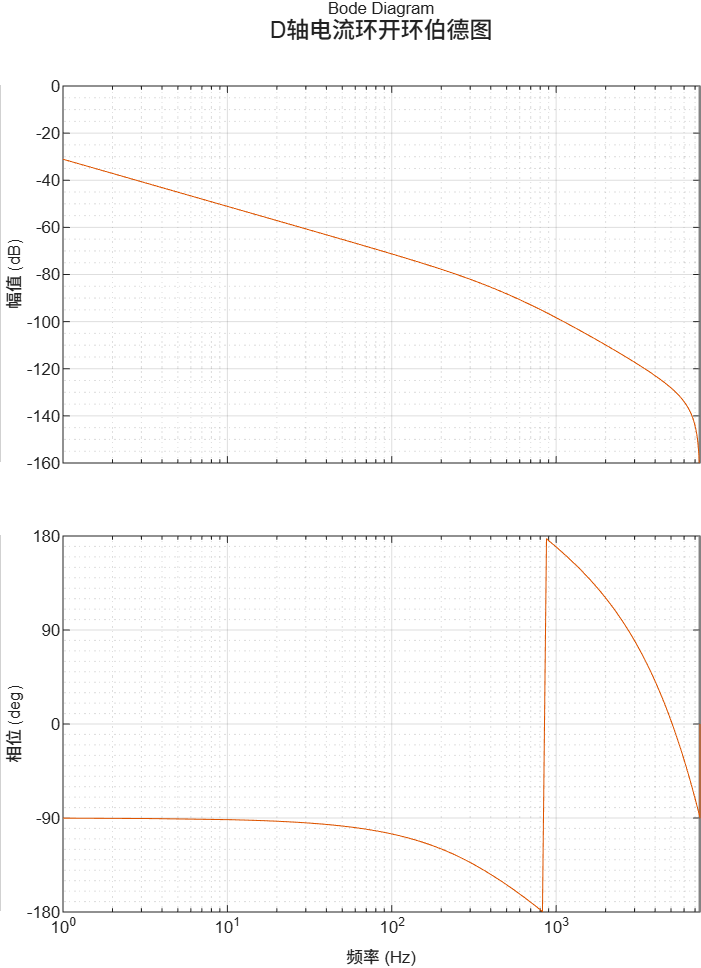
\includegraphics[width=0.5\textwidth]
    {图片/带积分环节的D轴等价被控对象开环频率特性.png}
    \caption{带积分环节的D轴等价被控对象开环频率特性}
\end{figure}

采用一阶超前校正控制\(C_{\mathrm{D}}(s)=K\cfrac{Ts+1}{\alpha Ts+1}\)，开环截止频率设定为1000Hz，以不低于40°的相位裕度为目标，
在1000Hz处提供最多60°的相位补偿，可以计算得到：
\begin{equation*}
    \begin{cases}
        \alpha = \cfrac{1-\sin(60°)}{1+\sin(60°)}=0.0718\\
        T = \cfrac{1}{2\pi\times 1000\sqrt{\alpha}} = 5.9391\times 10^{-4}
    \end{cases}
\end{equation*}

最后根据等价被控对象在1000Hz处的增益，调整放大系数K，最终可得带积分的D轴超前控制器：
\begin{equation*}
    C_{\mathrm{D}}(s)=\cfrac{12.95s+2.18\times 10^4}{4.265\times 10^{-5}s^2+s}
\end{equation*}

使用双线性变换离散化后得到\footnote{对于采用双线性变换离散化的控制器，积分环节对应为z=1的极点。因此要求离散后分母各个系数之和
要严格为零，否则z=1处的极点就会发生偏移，积分环节变为惯性环节。在正常工况下影响不大，但是在极端情况（如长时间堵转、积分严重
饱和）会导致系统行为失常。MATLAB默认显示四位有效数字，可能会导致精度损失，此时需要手动点开传递函数数据结构查看
更精确的值}：
\begin{equation*}
    C_{\mathrm{D}}(z)=\cfrac{5.998+0.6373z^{-1}-5.361z^{-2}}{1-1.1227z^{-1}+0.1227z^{-2}}
\end{equation*}

经过超前控制后的开环频率特性和闭环频率特性如下图所示。
\begin{figure}[H]
    \centering
    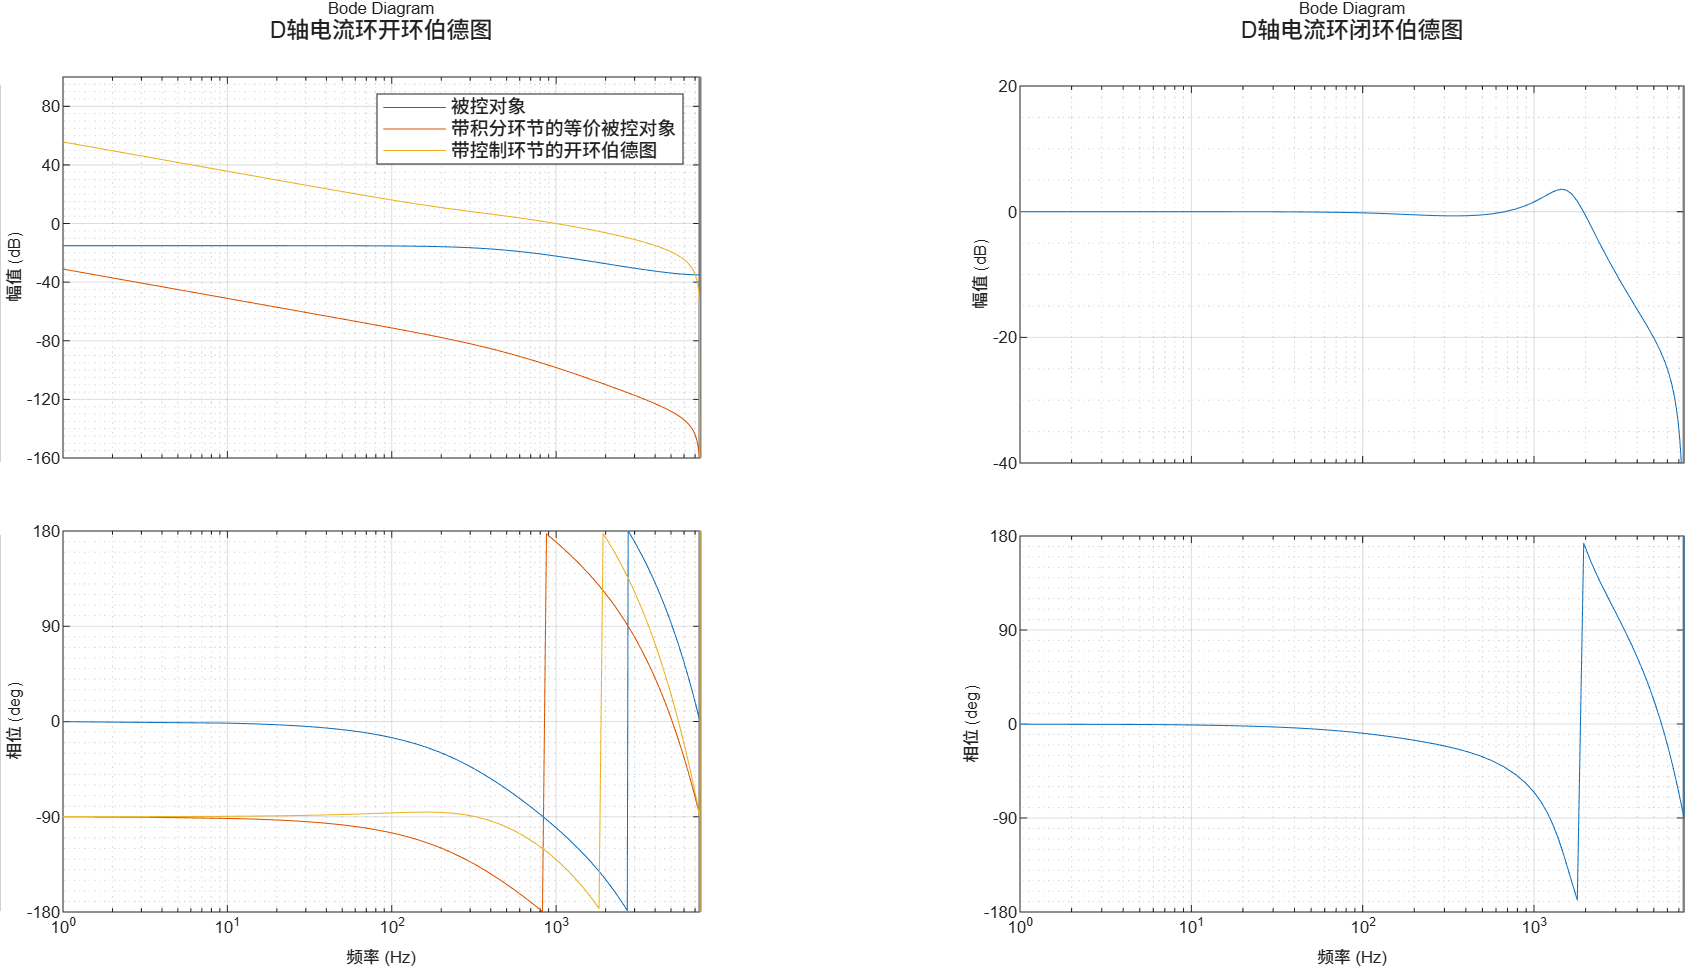
\includegraphics[width=\textwidth]
    {图片/D轴开-闭环频率特性.png}
    \caption{D轴开-闭环频率特性}
\end{figure}

矫正后，D轴电流环的开环截止频率1000.00073Hz，相位裕度49.46547°满足设计要求。相位穿越频率1883.94275Hz，
幅值裕度5.69334dB，闭环带宽2213.62137Hz。闭环前后的单位阶跃响应如下图所示。
\begin{figure}[H]
    \centering
    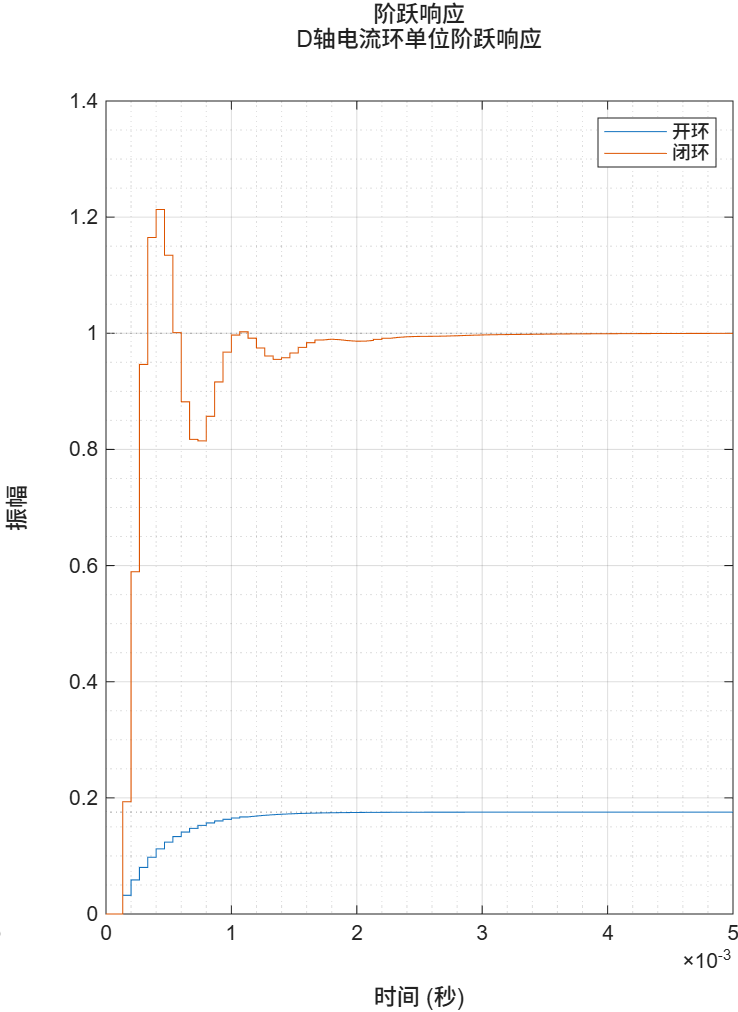
\includegraphics[width=0.5\textwidth]
    {图片/D轴开-闭环单位阶跃响应对比.png}
    \caption{D轴开-闭环单位阶跃响应对比}
\end{figure}

可以发现，通过带积分环节的超前校正控制器，使得能够无差跟踪给定信号，超调量21.3\%，调节时间为1.6ms，用一定的超调
换来了极快的响应速度。接下来考虑以±0.25A的方波电流给定信号（持续50个采样周期）进行测试，以评估实际系统响应和
建模准确性，结果如下图所示。
\begin{figure}[H]
    \begin{minipage}{0.5\textwidth}
        \centering
        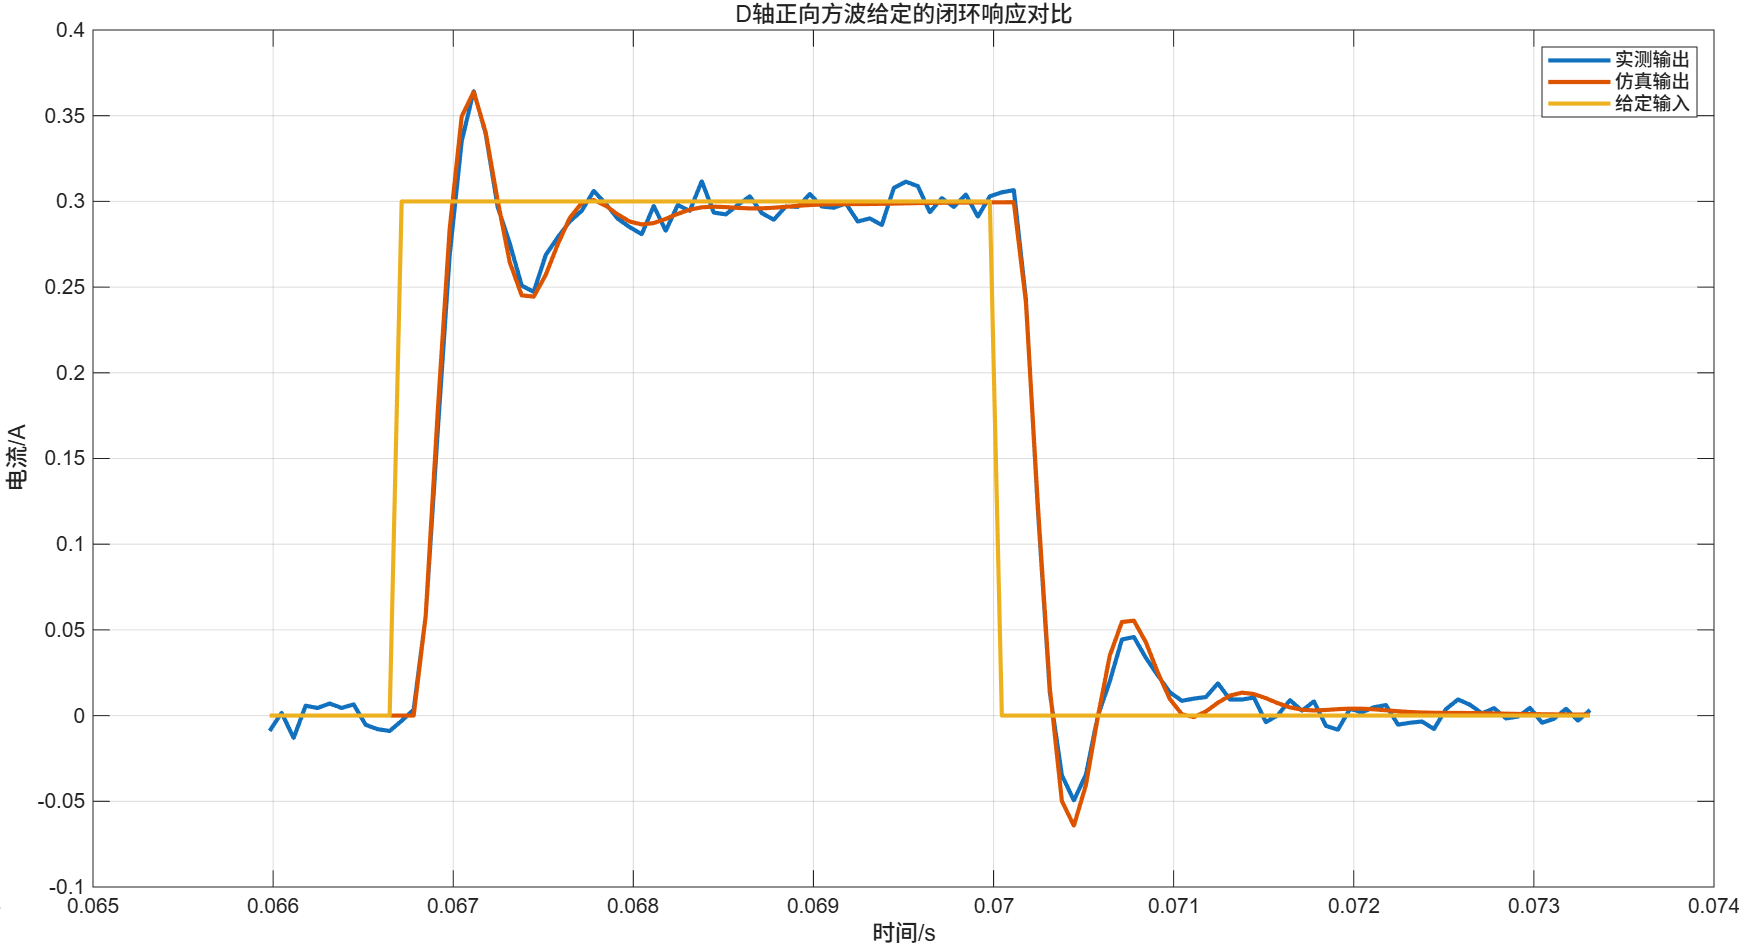
\includegraphics[width=\textwidth]
        {图片/D轴正向方波闭环验证.png}
        \caption{D轴正向方波闭环验证}
    \end{minipage}
    \begin{minipage}{0.5\textwidth}
        \centering
        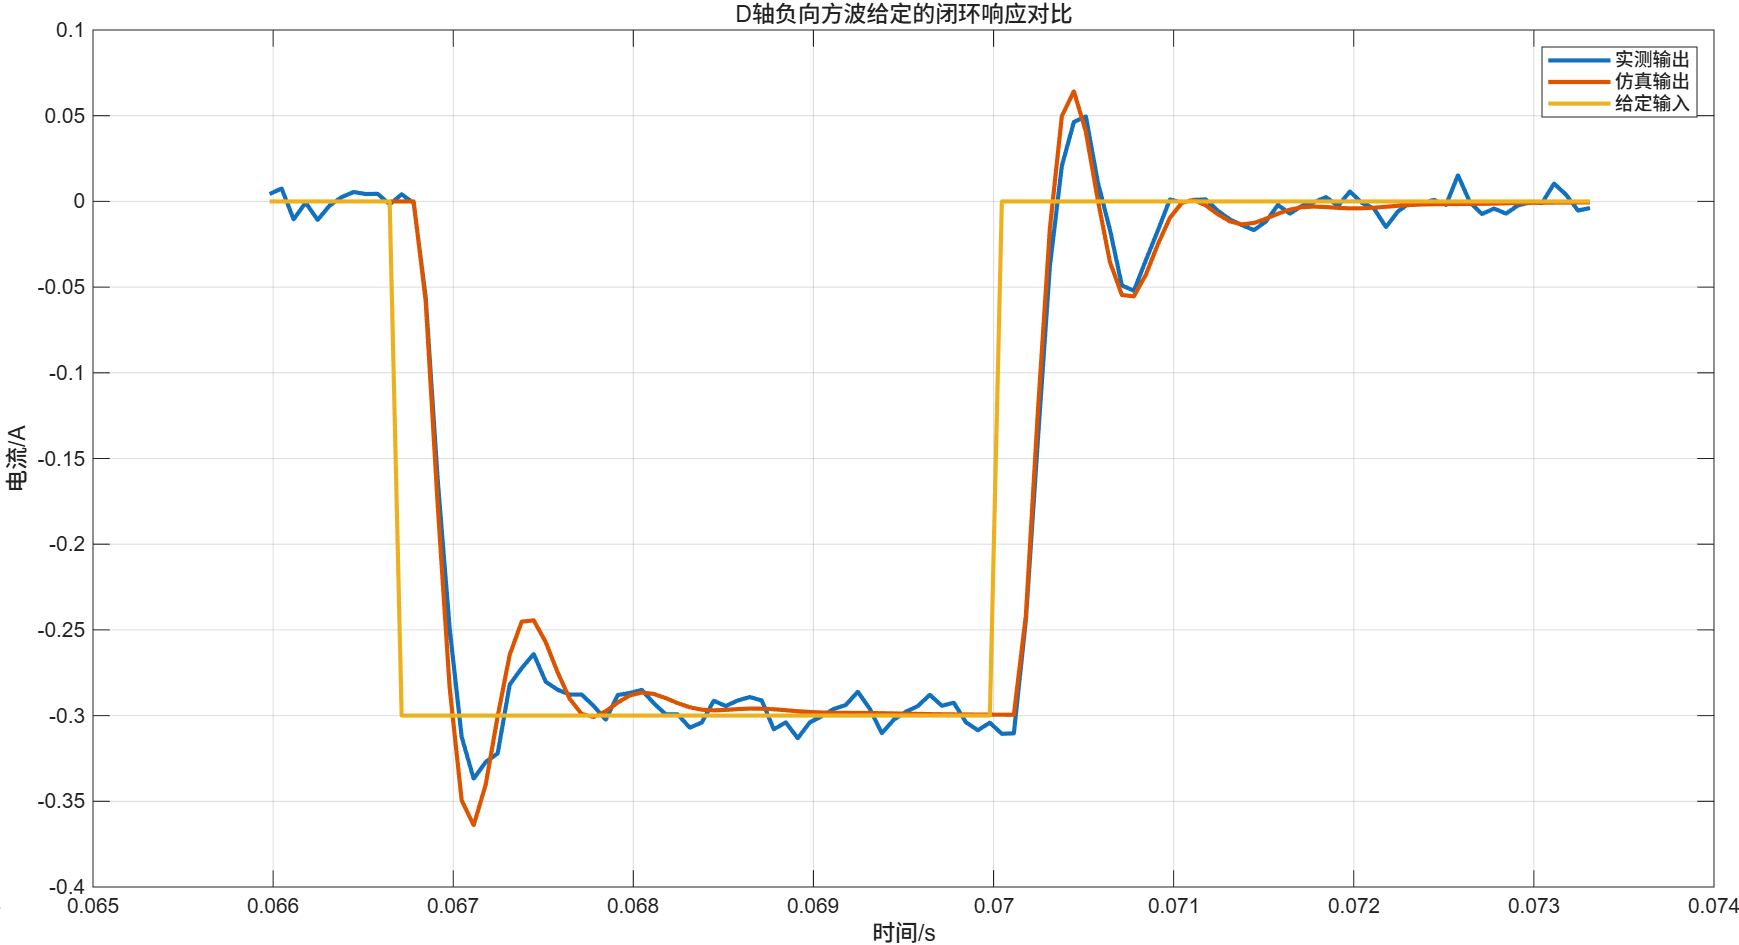
\includegraphics[width=\textwidth]
        {图片/D轴负向方波闭环验证.png}
        \caption{D轴负向方波闭环验证}   
    \end{minipage}
\end{figure}

据上图可知，由于存在采样噪声且进行闭环控制后系统对采样噪声的敏感度升高，导致实测电流波形有较大的波动。但在
整体趋势上和仿真波形一致。
正向方波中相关系数为99.88301\%，拟合优度95.15871\%；
负向方波中相关系数为99.73266\%，拟合优度92.69211\%，均为较高水平。

\subsubsection{Q轴频域矫正控制器设计与闭环验证}
Q轴电流环的传递函数为：
\begin{align*}
    G_{\mathrm{Q}}(z)&=(1-z^{-1})\mathcal{Z}[\cfrac{e^{-66.93\times10^{-6}s}}
        {s(5.70125+2.16828\times 10^{-3}s)(120\times 10^{-9}s+1)}]\\
        &=z^{-2}\cfrac{0.02805 + 0.0001482 z^{-1}+5.776\times 10^{-21}z^{-2}}{1- 0.8393 z^{-1}}
\end{align*}

与D轴同理，在电流环中串联积分环节\(I(z)\)以消除稳态误差，构造带积分环节的等价被控对象
\(I(z)G_{\mathrm{Q}}(z)\)，其开环频率特性如下图所示。
\begin{figure}[H]
    \centering
    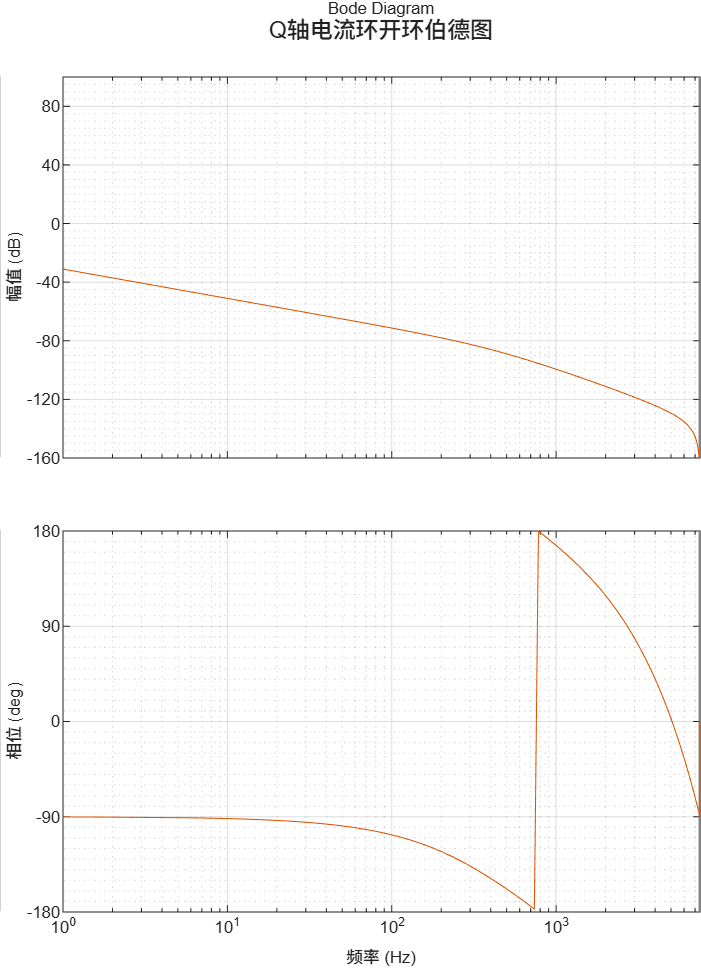
\includegraphics[width=0.5\textwidth]
    {图片/带积分环节的Q轴等价被控对象开环频率特性.png}
    \caption{带积分环节的Q轴等价被控对象开环频率特性}
\end{figure}

采用与D轴相同的一阶超前校正结构\(C_{\mathrm{Q}}(s)=K\cfrac{Ts+1}{\alpha Ts+1}\)，设计指标保持一致：
开环截止频率1000Hz，相位裕度不低于40°，在1000Hz处提供最多60°的相位补偿。\(\alpha\)和\(T\)
的取值与D轴完全相同（\(\alpha=0.0718\)，\(T=5.9391\times 10^{-4}\)），仅需根据Q轴等价被控对象
在1000Hz处的增益调整放大系数\(K\)。由于Q轴电感大于D轴（\(L_{\mathrm{q}}=2.16828\textrm{mH}>L_{\mathrm{d}}=1.86152\textrm{mH}\)），
Q轴RL电路的转折频率更低，1000Hz处的增益衰减更大，因此需要略高的\(K\)值补偿。最终可得带积分的
Q轴超前控制器：
\begin{equation*}
    C_{\mathrm{Q}}(s)=\cfrac{14.7s+2.474\times 10^4}{4.265\times 10^{-5}s^2+s}
\end{equation*}

使用双线性变换离散化后得到：
\begin{equation*}
    C_{\mathrm{Q}}(z)=\cfrac{6.808+0.7233z^{-1}-6.085z^{-2}}{1-1.1227z^{-1}+0.1227z^{-2}}
\end{equation*}

经过超前控制后的开环频率特性和闭环频率特性如下图所示。
\begin{figure}[H]
    \centering
    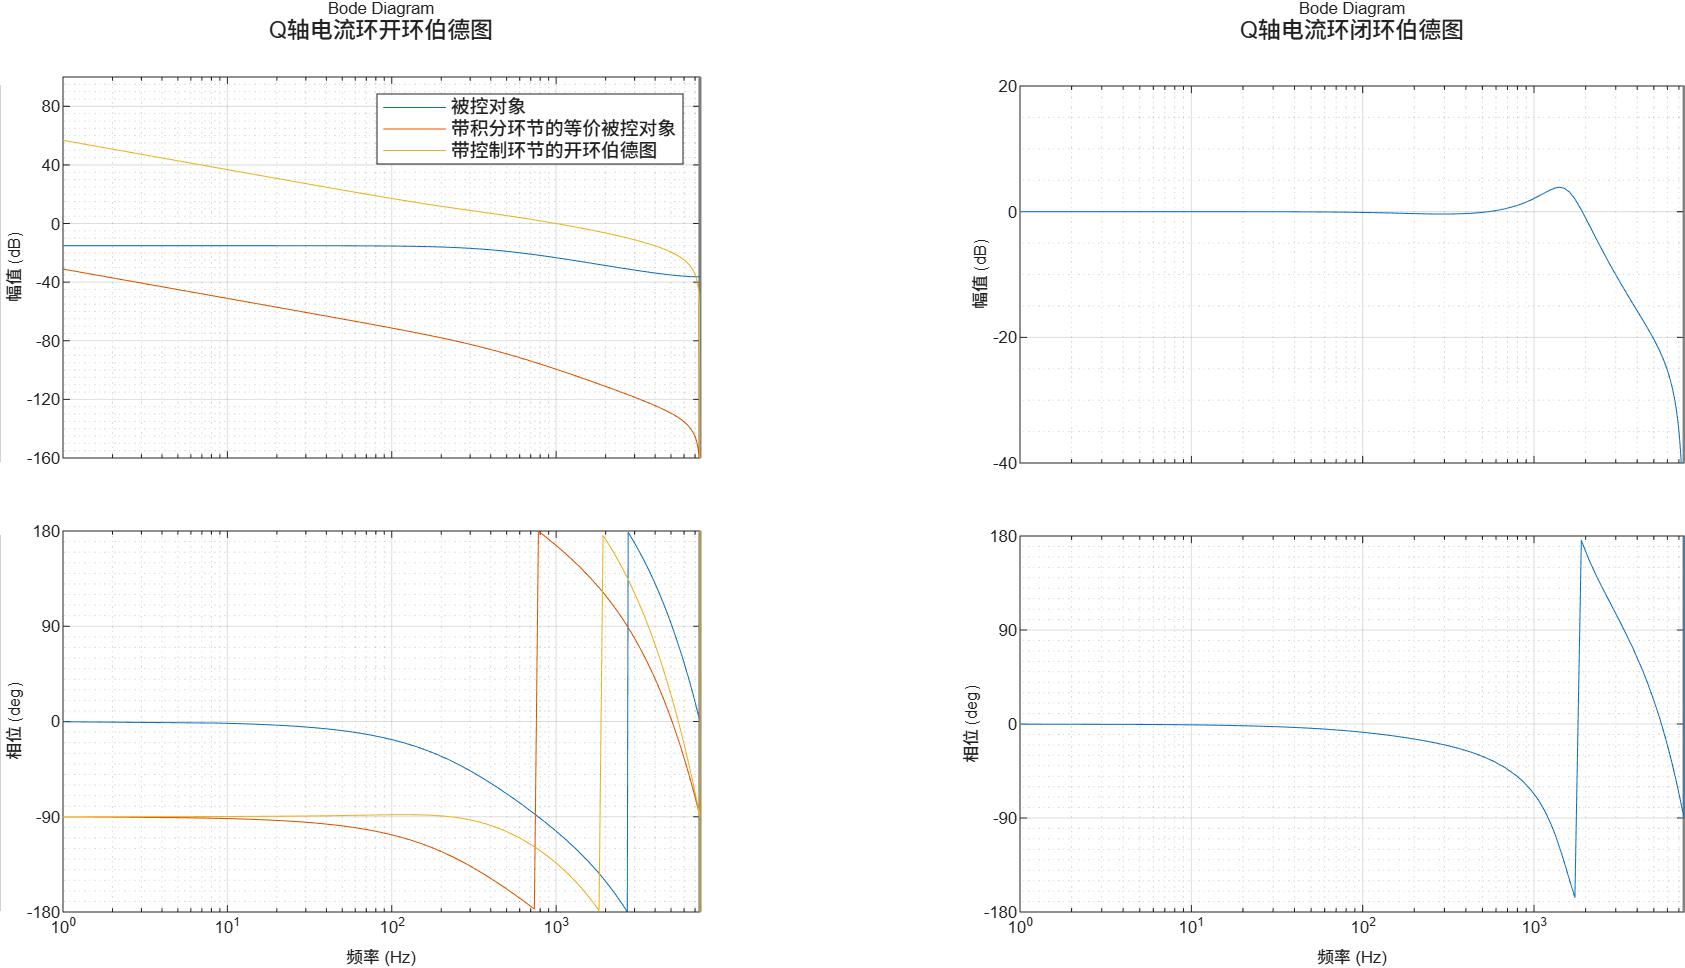
\includegraphics[width=\textwidth]
    {图片/Q轴开-闭环频率特性.png}
    \caption{Q轴开-闭环频率特性}
\end{figure}

矫正后，Q轴电流环的开环截止频率1000.00063Hz，相位裕度46.24331°满足设计要求。
相位穿越频率1848.20511Hz，幅值裕度5.65228dB，闭环带宽2179.71785Hz。
闭环前后的单位阶跃响应如下图所示。
\begin{figure}[H]
    \centering
    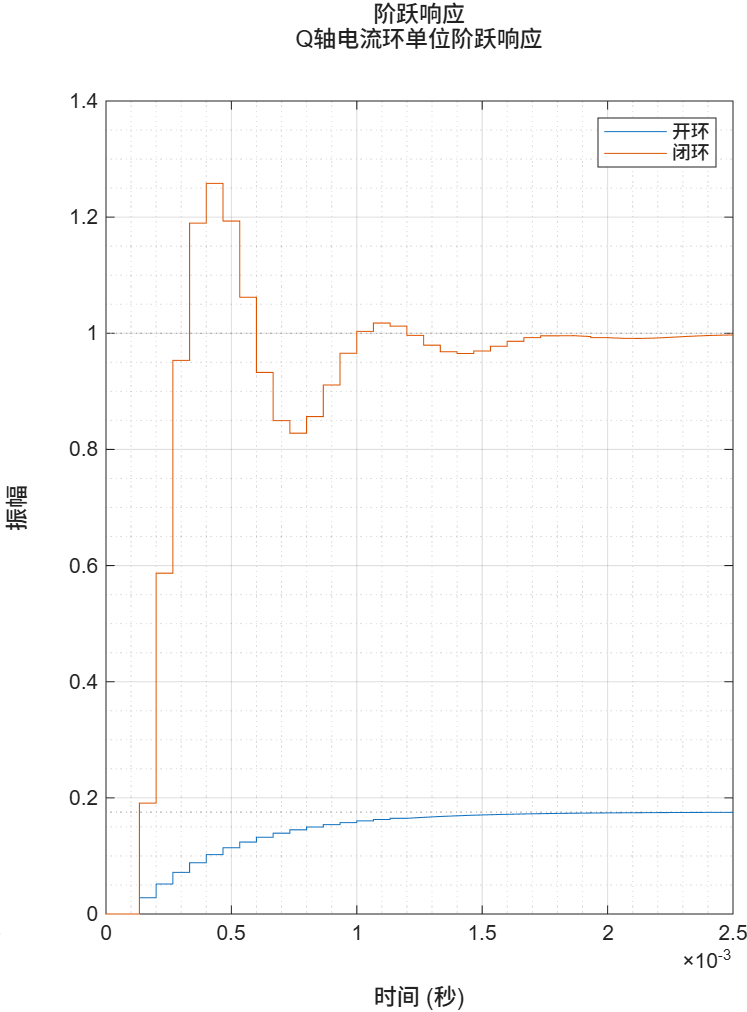
\includegraphics[width=0.5\textwidth]
    {图片/Q轴开-闭环单位阶跃响应对比.png}
    \caption{Q轴开-闭环单位阶跃响应对比}
\end{figure}

可以发现，Q轴闭环阶跃响应的超调量25.8\%，调节时间1.6ms，与D轴基本一致，这是因为
两者采用了相同的频域设计指标和校正器结构。

接下来以±0.25A的方波电流给定信号进行闭环跟踪测试。与D轴方波持续50个采样周期不同，
Q轴的方波仅持续5个采样周期\footnote{Q轴测试时电机会因电磁转矩而转动，方波持续时间过长将导致
转速累积升高，反电动势\(\omega_{\mathrm{e}}(\psi_{\mathrm{m}}+L_{\mathrm{d}}i_{\mathrm{d}})\)随之增大，削弱等效Q轴电压\(U_{\mathrm{q}}'\)中的激励分量，
迫使控制器持续增大\(U_{\mathrm{q}}\)以维持跟踪，最终进入饱和区，使系统非线性显著增强而难以进行线性仿真分析。
缩短方波持续时间可限制电机转角与转速的累积，将反电动势对等效RL电路模型的干扰控制在可忽略范围内。}。
闭环验证结果如下图所示。
\begin{figure}[H]
    \begin{minipage}{0.5\textwidth}
        \centering
        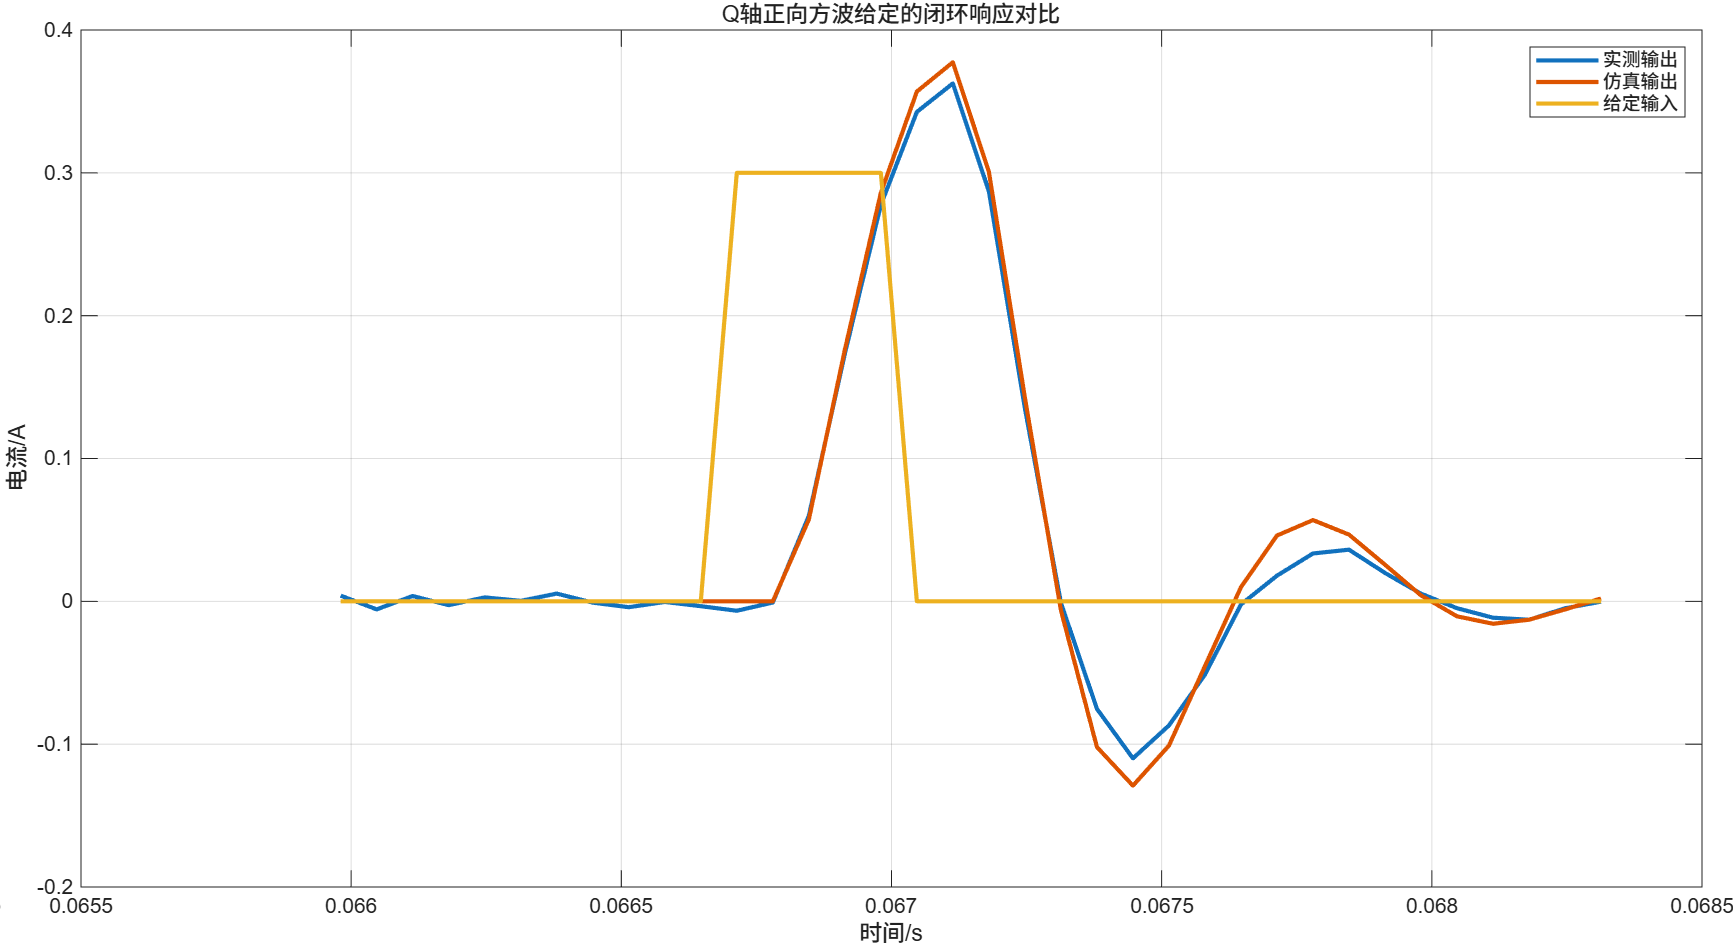
\includegraphics[width=\textwidth]
        {图片/Q轴正向方波闭环验证.png}
        \caption{Q轴正向方波闭环验证}
    \end{minipage}
    \begin{minipage}{0.5\textwidth}
        \centering
        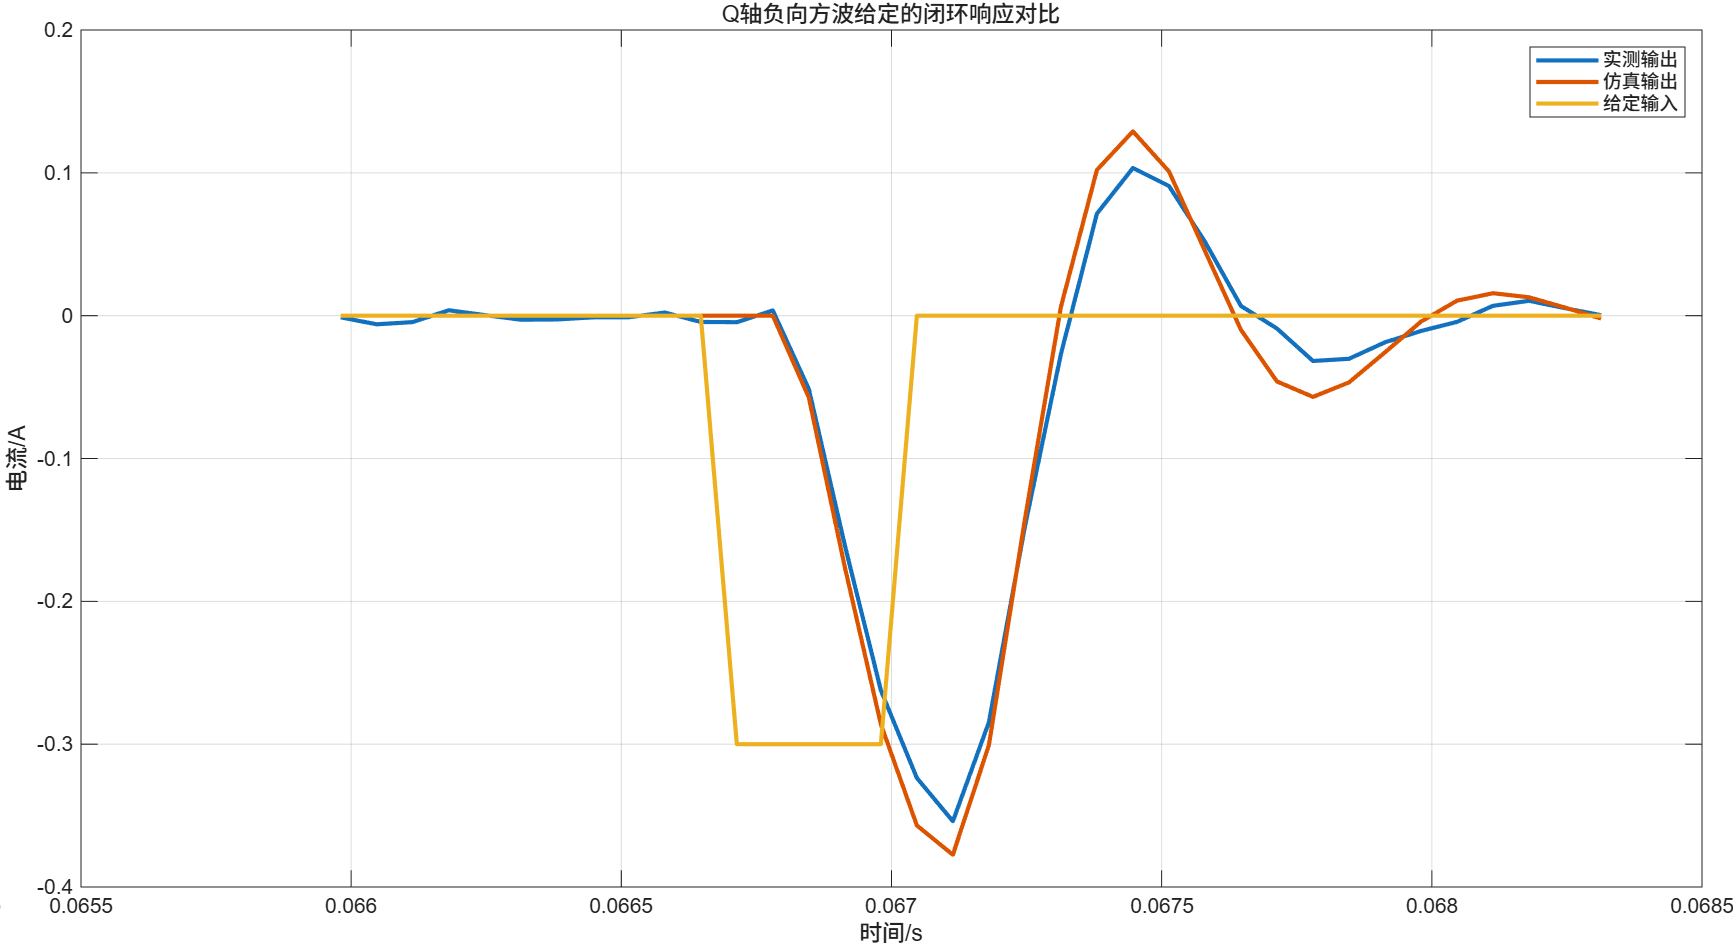
\includegraphics[width=\textwidth]
        {图片/Q轴负向方波闭环验证.png}
        \caption{Q轴负向方波闭环验证}
    \end{minipage}
\end{figure}

由于Q轴方波持续时间极短（5个采样周期仅约0.33ms），远小于闭环调节时间（1.6ms），
电流在每个脉冲内尚未到达稳态即被翻转，因此该测试实质上是暂态跟踪能力的验证，
而非稳态方波跟踪。实测曲线与仿真曲线的趋势吻合良好，
正向方波中相关系数为99.71872\%，拟合优度90.50733\%；
负向方波中相关系数为99.42643\%，拟合优度85.36039\%，
验证了Q轴频域校正控制器的瞬态响应有效性。

\subsection{速度环辨识理论分析}
虽然前文已经完成了Q轴电流环的闭环校正，但在速度环辨识中并未直接以电流给定\(i_{\mathrm{q}}^*\)作为激励
输入。其原因是Q轴电流控制器\(C_{\mathrm{Q}}(z)\)中含有积分环节，若以\(i_{\mathrm{q}}^*\)
\footnote{用上标*表示对某个物理量的给定/期望（如\(i_{\mathrm{d}}^*,i_{\mathrm{q}}^*,n^*\)），无上标*的表示实际值
（如\(i_{\mathrm{d}},i_{\mathrm{q}},n\)）。}
替代\(U_{\mathrm{q}}\)作为输入，辨识过程中积分器将持续累积\(i_{\mathrm{q}}^*\)与实际\(i_{\mathrm{q}}\)之间的跟踪误差并迅速
进入饱和区，使系统非线性显著增强，违背线性辨识的基本假设。因此，速度环的辨识仍以\(U_{\mathrm{q}}\)作为可操作变量。

速度环辨识的对象是机械部分的传递函数\(G_{\mathrm{m}}(s)\)，即从电磁转矩\(T_{\mathrm{e}}\)到转速\(n\)的传递函数。
由于电磁转矩无法直接测量，只能由实测电流重构。此外，反电动势\(\omega_{\mathrm{e}}\psi_{\mathrm{m}}\)构成物理闭环，
使得对该传递函数的直接辨识必然在闭环条件下进行，存在理论上的偏倚。

在空载情况下，电机的机械部分一般被建模为带有与速度成正比的粘滞摩擦环节，即一般认为传递函数为：
\begin{equation*}
    G_{\mathrm{m}}(s)=\cfrac{n(s)}{T_{\mathrm{e}}(s)}=\cfrac{1}{B+Js}
\end{equation*}

但是由于电机的机械部分非线性因素远超电气部分，上述假设在实际中往往无法成立分析。因此在这里将机械部分视为一个
阶次不定的系统，在特定工作点附近的局部线性化传递函数为\(G_{\mathrm{m}}(s)\)

在\(i_{\mathrm{d}}^*=0\)的条件下，\(U_{\mathrm{d}}\)用于维持理想化的\(i_{\mathrm{d}}=0\)条件，而\(U_{\mathrm{q}}\)用于控制\(i_{\mathrm{q}}\)，实现转矩环和速度环控制。
此时电磁转矩为\(T_{\mathrm{e}}=\cfrac{3}{2}p\psi_{\mathrm{m}}i_{\mathrm{q}}\propto i_{\mathrm{q}}\)为线性增益环节。而Q轴反电动势为
\(E=\omega_{\mathrm{e}}(\psi_{\mathrm{m}}+L_{\mathrm{d}}i_{\mathrm{d}})\)，在\(i_{\mathrm{d}}=0\)时可以简化为\(E=\omega_{\mathrm{e}}\psi_{\mathrm{m}}\propto \omega_{\mathrm{e}}\)也是线性增益环节。
考虑电角速度\(\omega_{\mathrm{e}}\)与转速\(n\)满足\(\omega_{\mathrm{e}}=\cfrac{\pi}{30}np\)，因此反电动势可以表示为
\(E=\cfrac{\pi}{30}np\psi_{\mathrm{m}}\propto n\)。

因此可以得到从\(U_{\mathrm{q}}\)到\(n\)在\(i_{\mathrm{d}}=0\)的理想化假设下系统框图：
\begin{figure}[H]
    \centering
    \begin{tikzpicture}[auto, node distance=3cm, >=latex']
        % 样式定义
        \tikzstyle{block} = [draw, rectangle, minimum height=3em, minimum width=3em, align=center]
        \tikzstyle{sum} = [draw, circle, node distance=1.5cm, minimum size=0.5em, inner sep=0pt]
        \tikzstyle{input} = [coordinate]
        \tikzstyle{output} = [coordinate]
        \tikzstyle{feedback} = [coordinate]

        % 放置节点
        \node [input, name=input] {};
        \node [sum, right of=input] (sum) {};
        \node [block, right of=sum] (RL) {\(\cfrac{1}{R_{\mathrm{s}}+L_{\mathrm{q}} s}\)};
        \node [block, right of=RL] (K) {\(\cfrac{3}{2}p\psi_{\mathrm{m}}\)};
        \node [block, right of=K] (Mech) {\(G_{\mathrm{m}}(s)\)};
        \node [output, right of=Mech] (output) {};
        \node [block, below of=K, node distance=1.5cm] (Kf) {\(\cfrac{\pi}{30}p\psi_{\mathrm{m}}\)};

        \draw [->] (input) -- node {\(U_{\mathrm{q}}\)} (sum);
        \draw [->] (sum) -- node {\(U_{\mathrm{q}}'\)} (RL);
        \draw [->] (RL) -- node {\(i_{\mathrm{q}}\)} (K);
        \draw [->] (K) -- node {\(T_{\mathrm{e}}\)} (Mech);
        \draw [->] (Mech) -- node [name=y] {\(n\)} (output);
        \draw [->] (y) |- (Kf);
        \draw [->] (Kf) -| node[pos=0.9] {\(-\)} node [pos=0.5] {\(E\)} (sum);
    \end{tikzpicture}
    \caption{\(i_{\mathrm{d}}=0\)假设下的Q轴电流-速度系统框图}
    \label{fig:Q轴电流-速度系统框图}
\end{figure}

按照先前直接辨识的思路，以\(U_{\mathrm{q}}\)为可操作输入量，测量\(T_{\mathrm{e}}\)视为实际输入，\(n\)为输出量，辨识
从\(T_{\mathrm{e}}\)到\(n\)的传递函数。设存在理想测量白噪声\(n_{\mathrm{T}}\)和
\(n_{\mathrm{n}}\)，无噪声的理论值为\(T_{0}\)和\(n_0\)。Ho-Kalman算法利用维纳-霍普夫方程估计系统的脉冲响应进行辨识，可以得到：
\begin{align*}
    n_k&=n_{0,k}+n_{\mathrm{n},k}\\
    &=T_0*g_{\mathrm{m}}+n_{\mathrm{n},k}\\
    &=(T_k-n_{\mathrm{T},k})*g_{\mathrm{m}}+n_{\mathrm{n},k}\\
    &=T_k*g_{\mathrm{m}}-n_{\mathrm{T},k}*g_{\mathrm{m}}+n_{\mathrm{n},k}
\end{align*}

对上式进行自相关运算，求解输入自功率谱密度函数和输入输出互功率谱密度函数，其商就是估计脉冲响应的离散傅里叶变换DTFT：
\begin{equation*}
    \hat{G}_{\mathrm{m}}(e^{\mathrm{j}\omega})=G_{\mathrm{m}}(e^{\mathrm{j}\omega})
    [1-\cfrac{\sigma_{\mathrm{T}}^2}{S_{T_{\mathrm{e}}T_{\mathrm{e}}}(e^{\mathrm{j}\omega})}]
\end{equation*}

其中\(\sigma_{\mathrm{T}}^2\)为测量噪声\(n_{\mathrm{T}}\)的方差，而\(S_{T_{\mathrm{e}}T_{\mathrm{e}}}(e^{\mathrm{j}\omega})\)
为实际测量值的自功率谱密度函数。由上式可知，在闭环情况下，
试图用开环的算法估计系统的脉冲响应，进而去分析系统的传递函数，结果将是有偏的。

需要注意的是，数学上有偏并不代表工程上不可行。若偏差很小，不影响工程分析，那么即使理论有偏在工程上也是可以接受的。如根据
图\ref{fig:Q轴电流-速度系统框图}，在\ref{sec:Q轴同步电感辨识}中进行的Q轴同步电感辨识方法也将是有偏的
\footnote{具体推导见\ref{sec:偏差直接重构中间到中间/输出的偏倚性分析}。}，但在开环和闭环验证中
均证实了辨识结果的有效性。因此，需要相干函数评估辨识结果的工程可用性：
\begin{equation}
    \gamma_{xy}^2(\omega)=\frac{|S_{xy}(e^{\mathrm{j}\omega})|^2}{S_{xx}(e^{\mathrm{j}\omega})\,S_{yy}(e^{\mathrm{j}\omega})}
    \label{eq:相干函数定义}
\end{equation}

其中\(S_{xy}(e^{\mathrm{j}\omega})\)为互功率谱密度，\(S_{xx}(e^{\mathrm{j}\omega})\)和\(S_{yy}(e^{\mathrm{j}\omega})\)为自功率谱密度。
相干函数满足\(0\le \gamma_{xy}^2(\omega)\le 1\)，在某个频点的值越接近1，说明输出信号中该频点的分量可以被输入信号线性解释的比例越高，
使用维纳-霍普夫方程估计脉冲响应序列在这个频点的可信度也越高。相干函数作为信噪比度量的含义、与偏置因子之间的联系详见\ref{sec:相干函数与估计质量的评估}。

为对比不同辨识策略在反电动势造成的闭环结构下的表现，考虑四种候选的待辨识传递函数，并分别计算其相干函数。这四种待辨识传递函数取自同一物理系统
（FOC控制下的永磁同步电机），覆盖了辨识问题中可能的输入输出选取方式，并在以下维度上彼此不同：
输入是给定还是闭环内信号、输入是直接测量还是重构、辨识工作在开环还是闭环、关注频段属于电路模态还是
机械模态。相干函数\(\gamma_{xy}^2\)经输入输出功率谱归一化，恰好可作为统一衡量这四种待辨识传递函数“输出被输入线性解释的比例”
的公共标尺。四种待辨识传递函数的差异汇总如下表所示。
\footnote{直接法辨识中选用\(i_\mathrm{q}\)而不是\(T_{\mathrm{e}}\)是因为电磁转矩无法直接测量，需要从电流中乘以常数得到，两者成正比
关系，因此分析从\(i_{\mathrm{q}}\)到\(n\)的相干函数即可。} 
\begin{table}[H]
    \centering
    \begin{tabular}{|c|c|c|c|}
        \hline
        通道 & 输入/输出 & 输入来源与结构 & 关注频段\\
        \hline
        开环基准（D轴同步电感） & \(U_{\mathrm{d}}/i_{\mathrm{d}}\) & 外部给定，开环 & 电路模态 \(100\sim3000\)Hz\\
        \hline
        重构等效输入（Q轴同步电感） & \(U_{\mathrm{q}}'/i_{\mathrm{q}}\) & 重构输入，闭环 & 电路模态 \(100\sim3000\)Hz\\
        \hline
        直接法（机械传递函数） & \(i_{\mathrm{q}}/n\) & 闭环内部测量，闭环 & 机械模态 \(1\sim300\)Hz\\
        \hline
        间接法（机械传递函数） & \(U_{\mathrm{q}}/n\) & 闭环外部给定，闭环 & 机械模态 \(1\sim300\)Hz\\
        \hline
    \end{tabular}
    \caption{四种候选待辨识传递函数特点对比}
    \label{tab:四种候选待辨识传递函数特点对比}
\end{table}

下面对这四种通道作具体说明：
\begin{itemize}
    \item 开环辨识基准（D轴同步电感\(L_{\mathrm{d}}\)辨识）：D轴电路方程为
\(u_{\mathrm{d}}=R_{\mathrm{s}}i_{\mathrm{d}}+L_{\mathrm{d}}\cfrac{\dd i_{\mathrm{d}}}{\dd t}\)，在\(i_{\mathrm{q}}=0\)条件下无电磁转矩、
无转动、无反电动势，交叉耦合项\(\omega_{\mathrm{e}}L_{\mathrm{q}}i_{\mathrm{q}}=0\)，D轴RL电路为纯开环结构，
辨识结果理论上无偏，可作为相干函数的理想参考基准。
    \item 重构等效输入法（Q轴同步电感\(L_{\mathrm{q}}\)辨识）：通过计算等效输入电压
\(U_{\mathrm{q}}'=U_{\mathrm{q}}-\omega_{\mathrm{e}}(L_{\mathrm{d}}i_{\mathrm{d}}+\psi_{\mathrm{m}})\)辨识从\(U_{\mathrm{q}}'\)到\(i_{\mathrm{q}}\)的传递函数。
    \item 直接法：以测量的\(i_{\mathrm{q}}\)为输入、转速\(n\)为输出，直接辨识从\(i_{\mathrm{q}}\)到\(n\)的
传递函数。
    \item 间接法闭环辨识：先辨识从\(U_{\mathrm{q}}\)到\(n\)的闭环传递函数，再根据已确定的Q轴
电流传递函数反推机械部分的传递函数\(G_{\mathrm{m}}(s)\)。
\end{itemize}

将相干函数满足\(\gamma^2_{\text{dB}} > -0.5\text{dB}\)（即\(\gamma^2 \ge 0.89\)）视为估计
可靠区间。

在对机械模态的辨识通道进行比较之前，先对第四章已完成的电路模态辨识（D/Q轴同步电感）结果进行相干函数评估，目的有二。
其一，D轴辨识在\(i_{\mathrm{q}}=0\)下无电磁转矩、无反电动势，系统处于纯开环，辨识结果理论上无偏，是相干函数这一评估方法在
实测数据上的标定基准。其二，Q轴辨识通过重构等效输入打破反电动势闭环，属于“理论有偏但工程上接近无偏”的例子，其相干函数可作为
后续机械辨识中判断是否工程可接受的参考。

对于电路模态（DQ轴的同步电感辨识），在\(100\text{Hz}\sim 3000\text{Hz}\)
范围内进行分析，该频段以RL电路转折频率为中心，覆盖了电流动态的主要信息区间。DQ轴同步电感辨识的相干函数如下所示。

\begin{figure}[H]
    \begin{minipage}{0.5\textwidth}
        \centering
        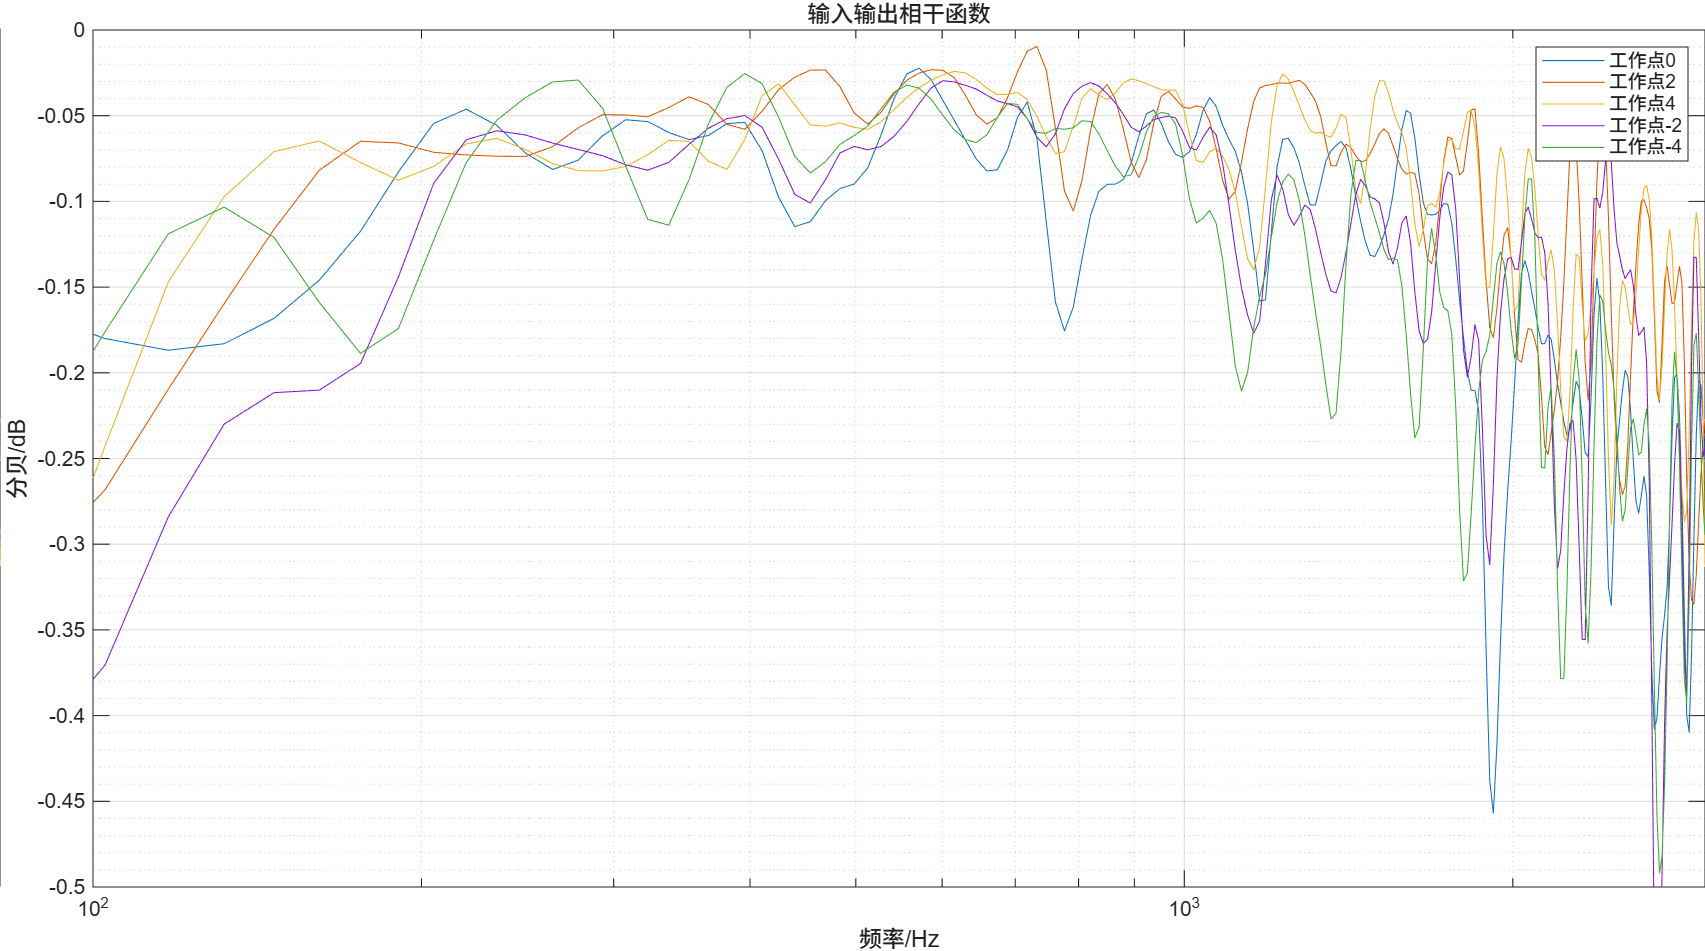
\includegraphics[width=\textwidth]
        {图片/D轴同步电感辨识相干函数.png}
        \caption{D轴同步电感辨识的相干函数}
        \label{fig:D轴同步电感辨识的相干函数}
    \end{minipage}
    \begin{minipage}{0.5\textwidth}
        \centering
        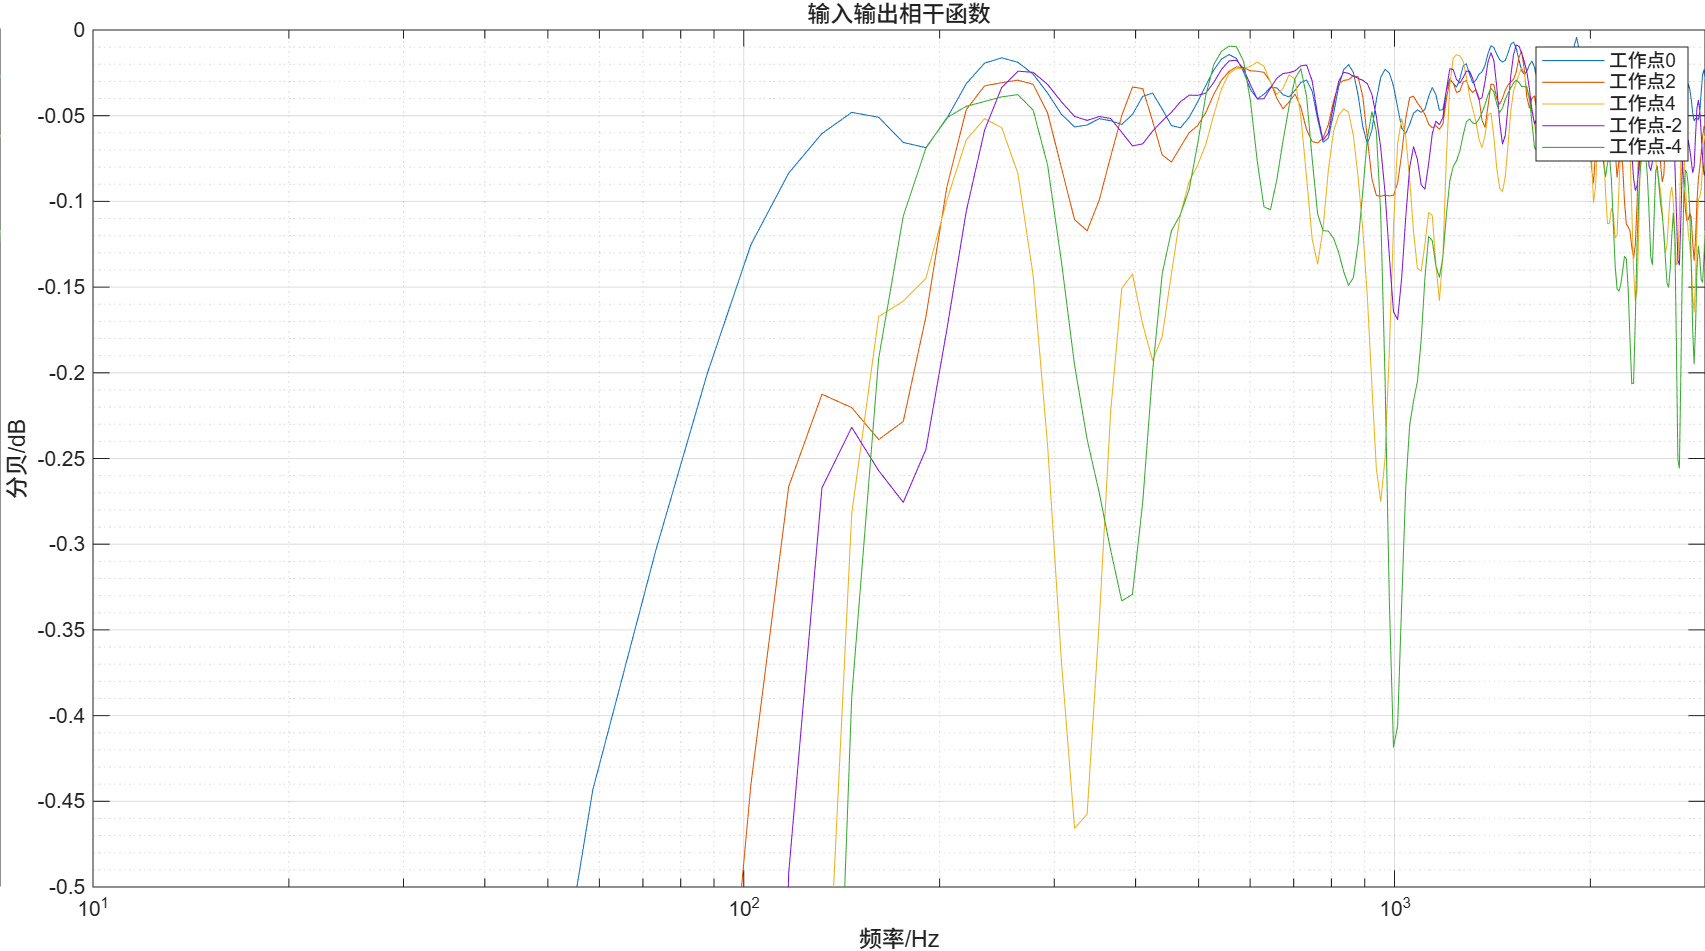
\includegraphics[width=\textwidth]
        {图片/Q轴同步电感辨识相干函数.png}
        \caption{Q轴同步电感辨识的相干函数}
        \label{fig:Q轴同步电感辨识的相干函数}
    \end{minipage}
\end{figure}

可以发现，D轴辨识时无电磁转矩、系统开环，相干函数在关注频段内均满足
\(\gamma^2_{\text{dB}} > -0.5\,\text{dB}\)，信噪比高，辨识可信度高。
Q轴辨识通过重构等效输入近似为开环（但是闭环的物理结构依然存在），相干函数整体较D轴有所下降，
且在出现相干函数谷值（如1kHz附近）。但在电路模态的核心频段（\(400\text{Hz}\sim
800\text{Hz}\)，即RL转折频率附近），Q轴相干函数仍能维持在\(-0.5\,\text{dB}\)
以上，说明即使理论有偏，工程上该偏差可以近似忽略。

接下来分析直接法与间接法在反电动势闭环结构下的表现，工作点取
\(U_{\mathrm{q}} = \pm 2\,\text{V}, \pm 4\,\text{V}\)
\footnote{相较于电路模态辨识少了0V工作点。0V附近静摩擦、转矩死区等
非线性因素主导，辨识结果与其他工作点截然不同，因此不纳入考虑。}
仍将\(\gamma^2_{\text{dB}} > -0.5\,\text{dB}\)视为工程可靠区间。机械动态远慢于电气动态，
其转折频率通常在数赫兹至数十赫兹量级，选取\(1\,\text{Hz}\sim 300\,\text{Hz}\)覆盖机械动态的主要信息区间。相干函数如下所示。
\begin{figure}[H]
    \begin{minipage}{0.5\textwidth}
        \centering
        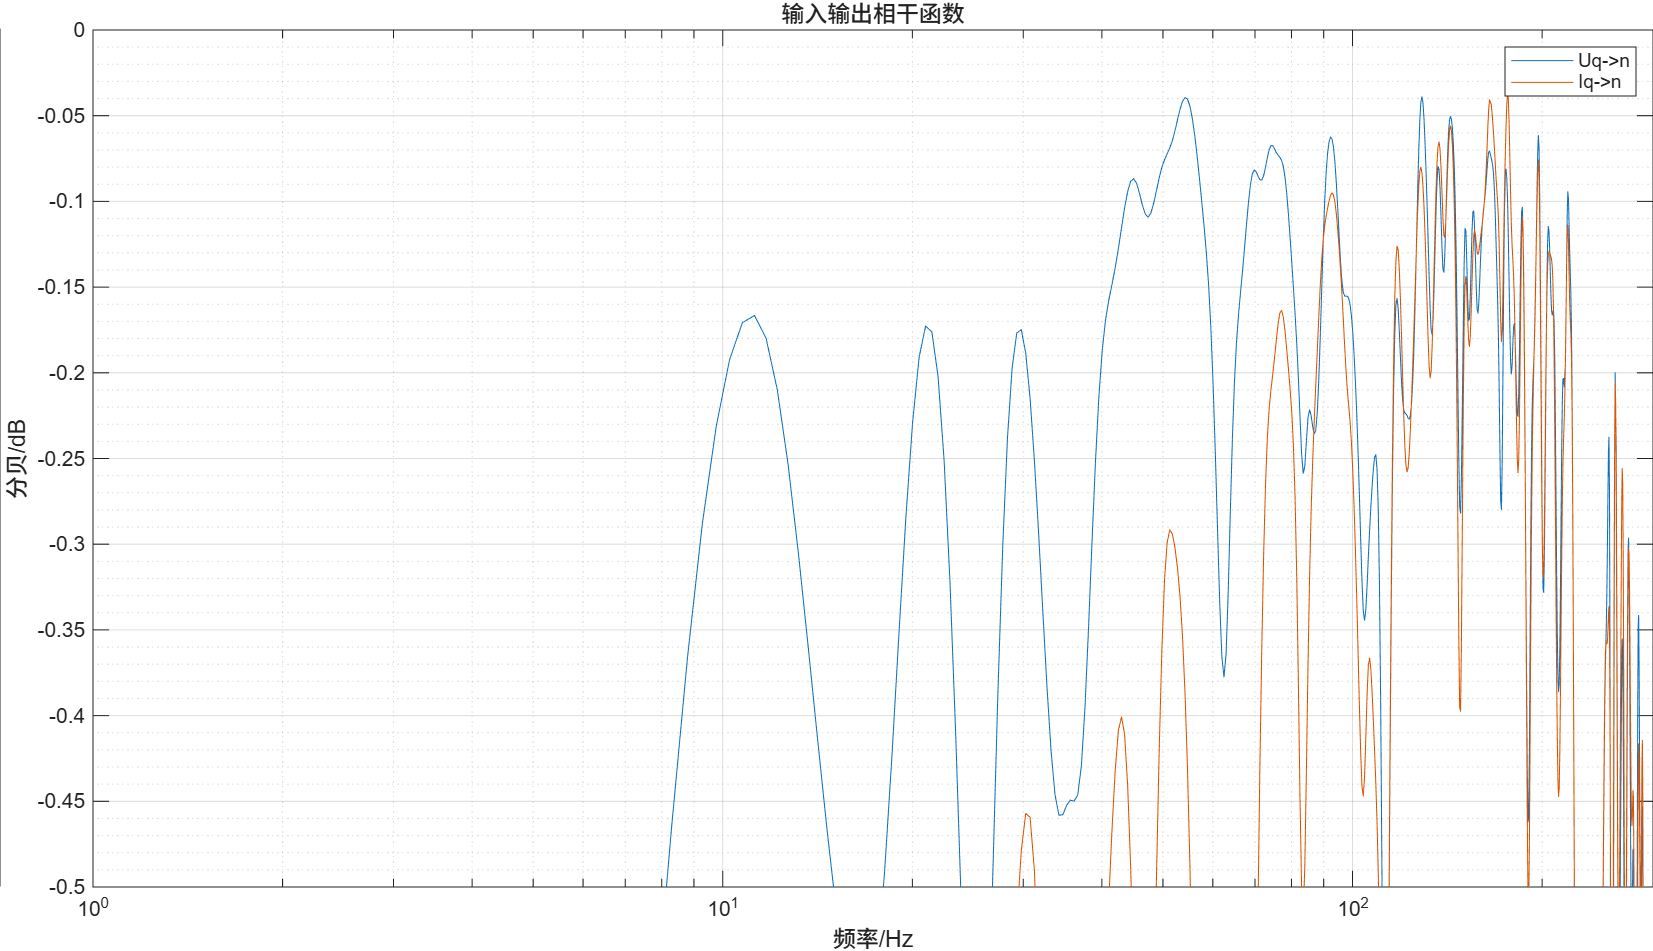
\includegraphics[width=\textwidth]
        {图片/速度环相干函数（-4V）.png}
        \caption{速度环相干函数（-4V）}
        \label{fig:速度环相干函数（-4V）}
    \end{minipage}
    \begin{minipage}{0.5\textwidth}
        \centering
        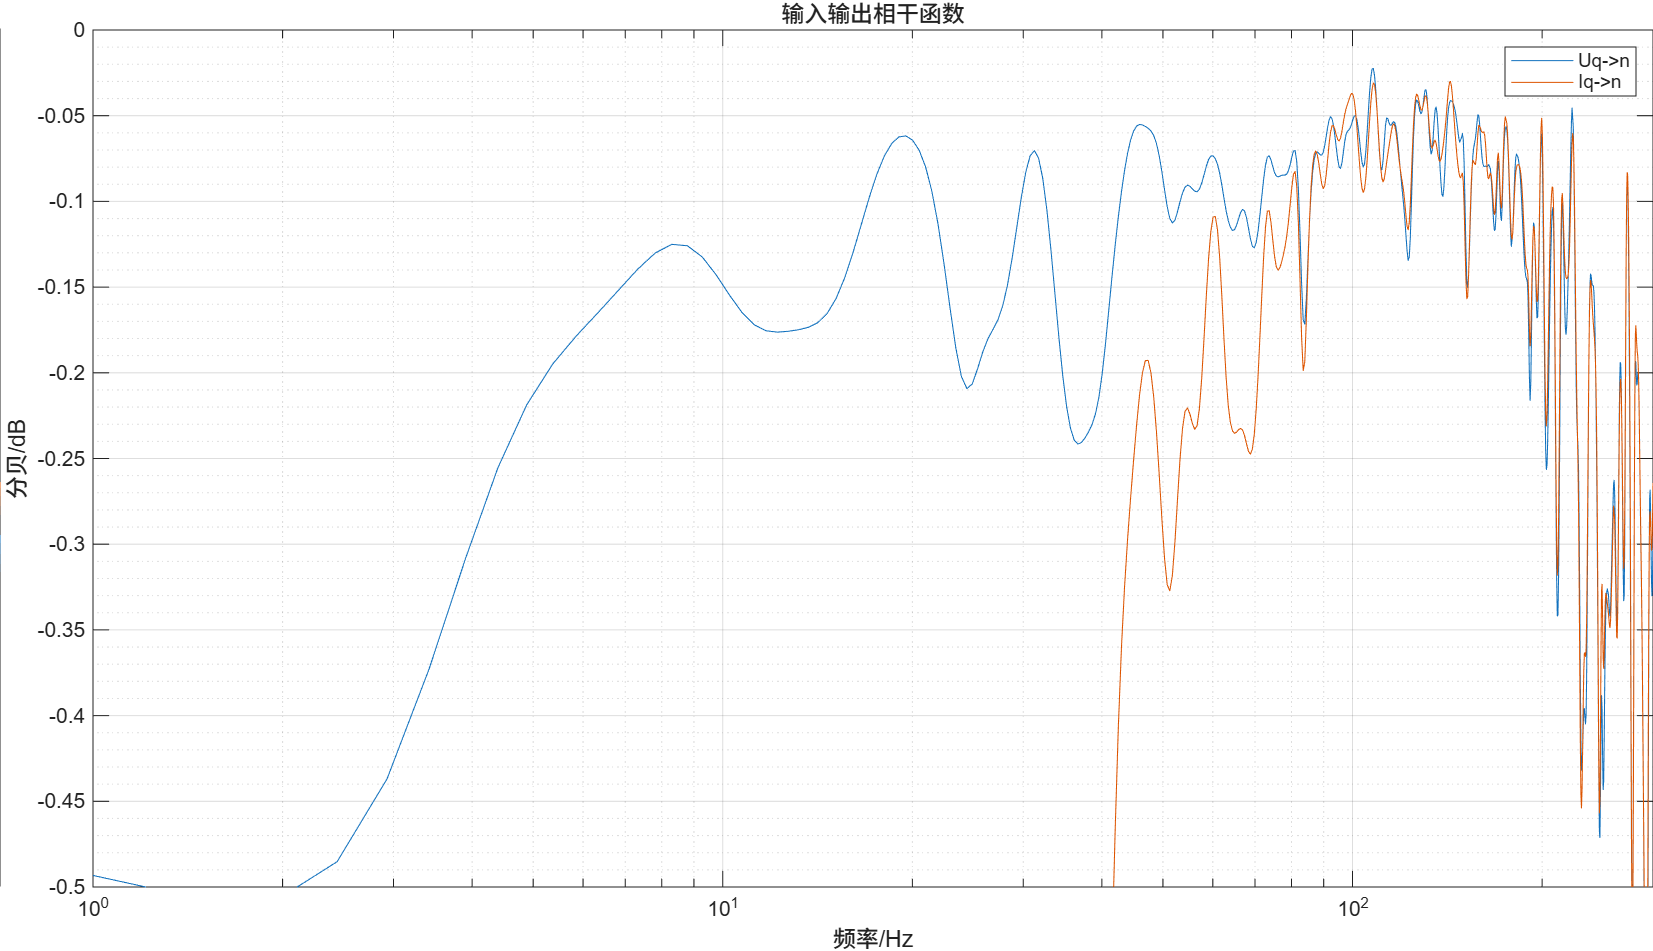
\includegraphics[width=\textwidth]
        {图片/速度环相干函数（-2V）.png}
        \caption{速度环相干函数（-2V）}
        \label{fig:速度环相干函数（-2V）}
    \end{minipage}
\end{figure}
\begin{figure}[H]
    \begin{minipage}{0.5\textwidth}
        \centering
        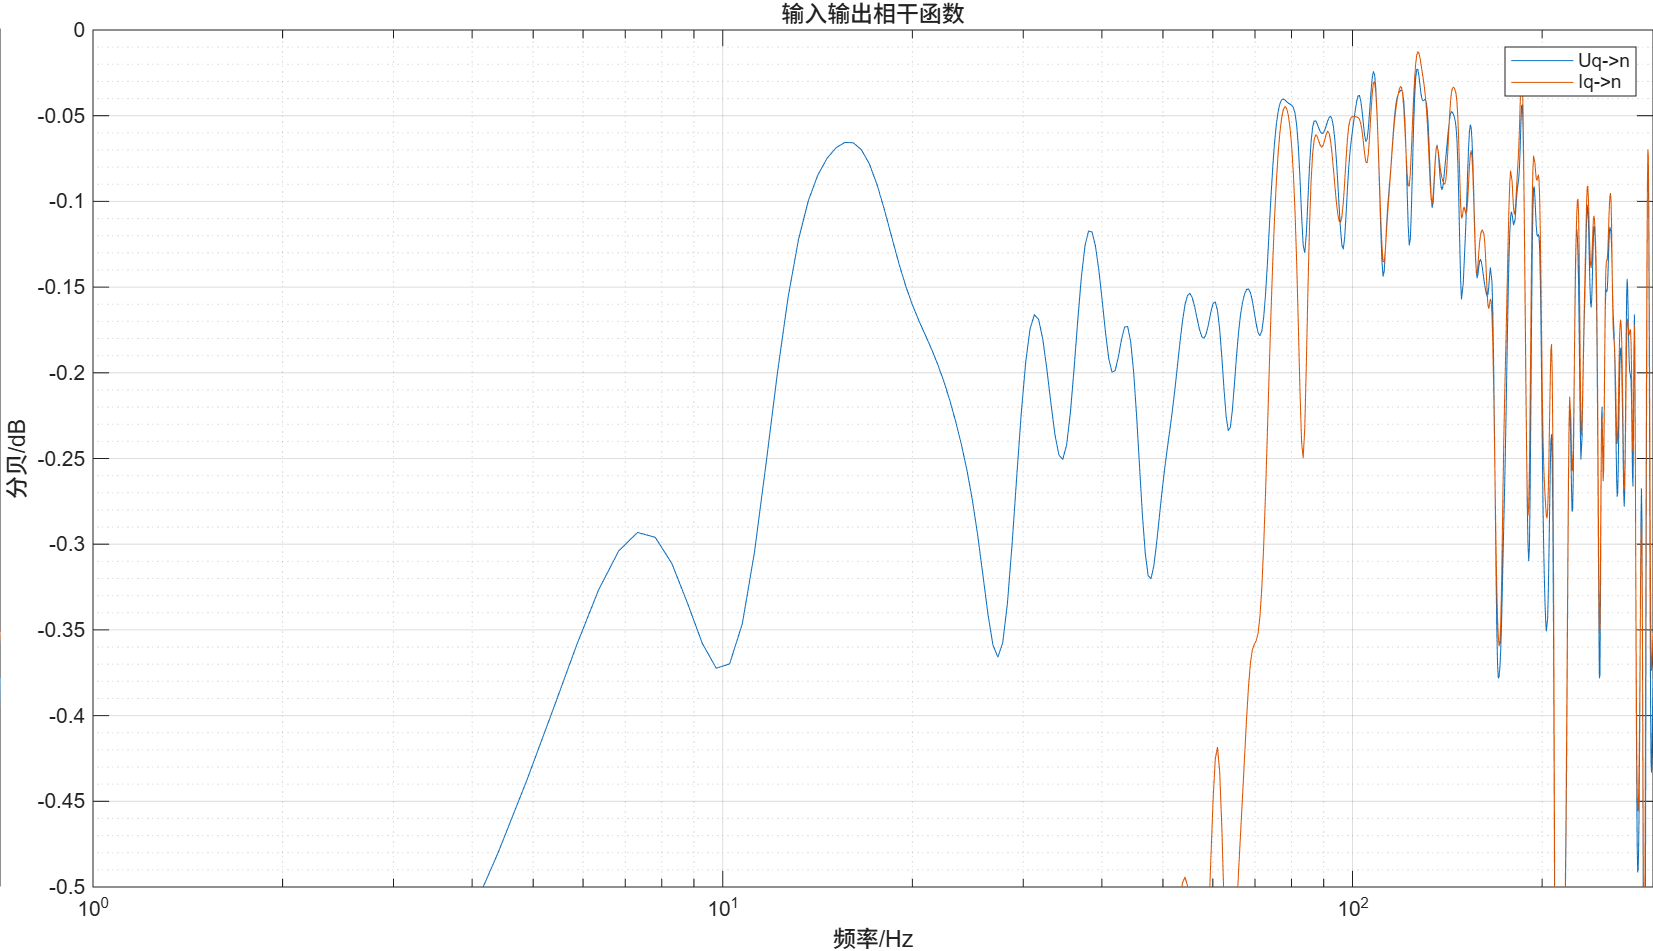
\includegraphics[width=\textwidth]
        {图片/速度环相干函数（2V）.png}
        \caption{速度环相干函数（2V）}
        \label{fig:速度环相干函数（2V）}
    \end{minipage}
    \begin{minipage}{0.5\textwidth}
        \centering
        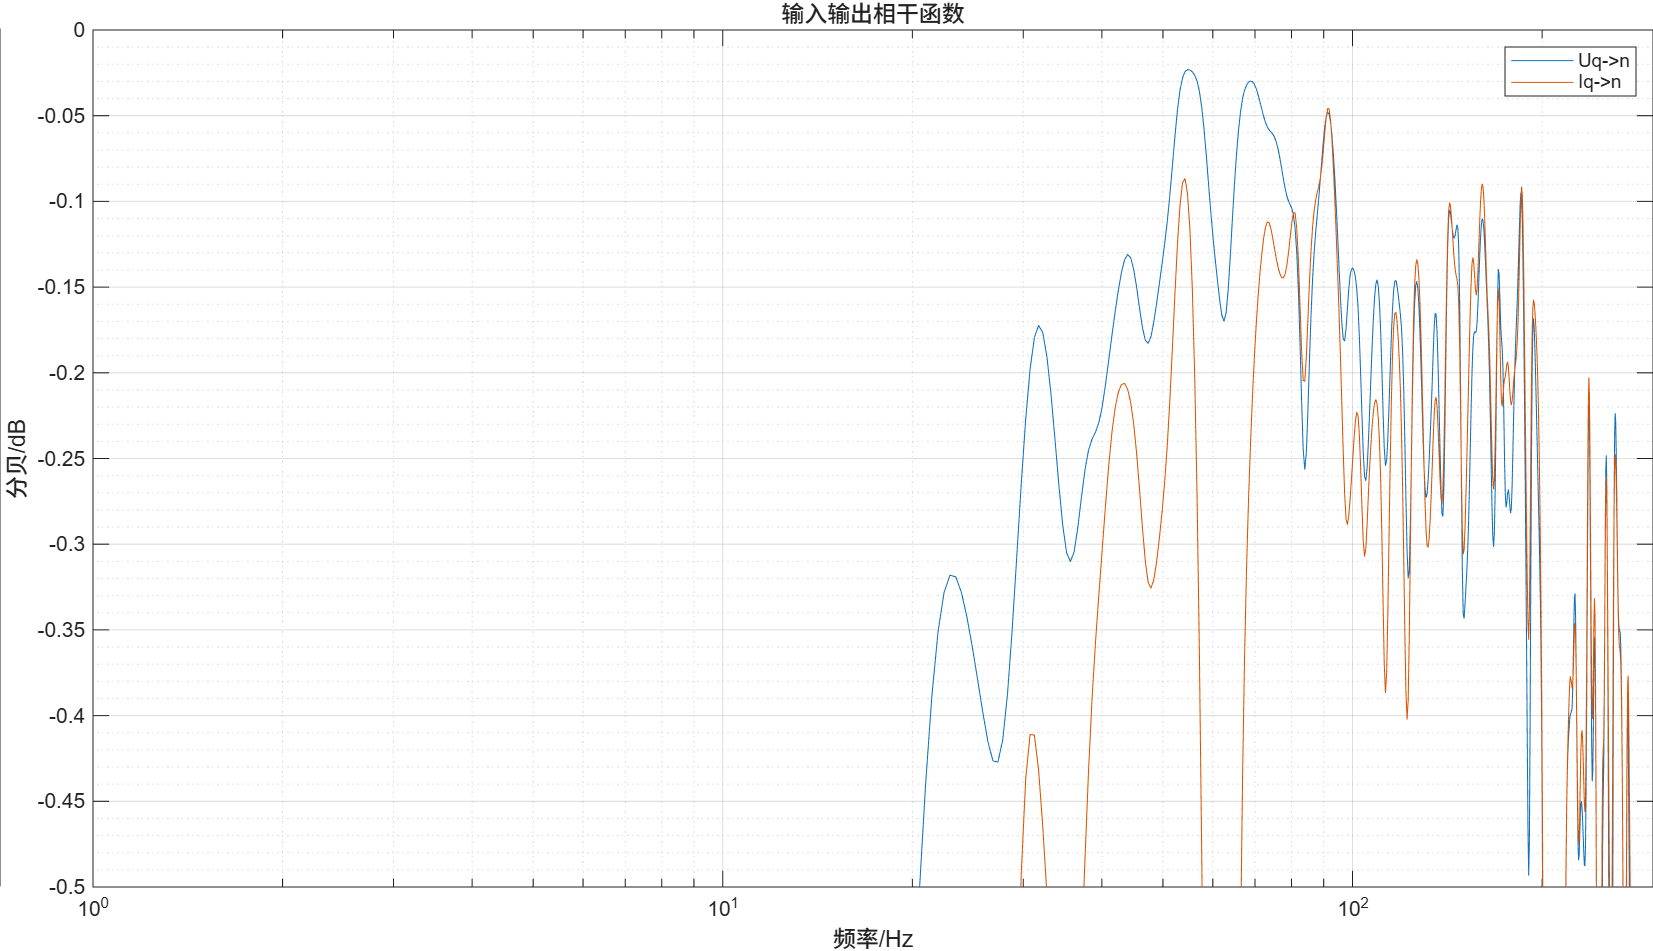
\includegraphics[width=\textwidth]
        {图片/速度环相干函数（4V）.png}
        \caption{速度环相干函数（4V）}
        \label{fig:速度环相干函数（4V）}
    \end{minipage}
\end{figure}

可以发现，直接法的相干函数在核心频段（\(10\,\text{Hz}\sim 100\,\text{Hz}\)）内
普遍较低，估计质量不可靠；间接法的相干函数虽整体优于直接法，
但仍明显低于电路模态的辨识结果。两者在机械动态中相干函数整体偏低，根本原因
在于机械部分的非线性因素（静摩擦、转矩死区、机械系统阶次不定等）无论从数量
还是强度均远超电路部分。
\footnote{另一种理解两者差异的角度是奇异摄动。电机的电路部分和机械部分时间常数尺度差异大，
（电路时间常数\(\cfrac{L_{\mathrm{q}}}{R_{\mathrm{s}}}\approx 0.3\text{ms}\)，而根据后续机械部分传递函数的主导极点
可知主导时间常数约\(\cfrac{1}{30}\text{s}=33.33\text{ms}\)，分离比\(\cfrac{0.3}{33.33}\approx 0.009\ll 1\)）
构成天然奇异摄动系统。辨识快模态（电路部分）时，慢模态（转速）在电气激励时间尺度上近似不变，
反电动势近似为常数，反馈回路基本没有激活。辨识慢模态（机械部分）时，
转速随激励同步变化，反电动势反馈回路在机械时间尺度上被完全激活，辨识结果可靠性显著降低。}
而直接法在闭环情况下还存在数学可证明的严格有偏，因此相干函数值更低。

综上，对机械传递函数的辨识应优先采用间接法：先辨识
\(U_{\mathrm{q}}\to n\)的闭环传递函数，再从已确定的Q轴电路传递函数中代数反推
\(G_{\mathrm{m}}(s)\)。间接法的优势是根本性的，如\ref{sec:输入直接到输出}所述，当以给定无噪信号
\(U_{\mathrm{q}}\)作为输入时，输入与输出测量噪声不相关，维纳-霍普夫方程能够无偏估计该通道的脉冲响应。

\subsection{速度环被控对象辨识与开环验证}
\subsubsection{\(i_{\mathrm{d}}=0\)理想化假设分析}
前文建立了基于\(i_{\mathrm{d}}^*=0\)假设的间接法辨识框架：将\(U_{\mathrm{q}}\)到\(n\)的通道建模为
反电动势闭环结构，其核心在于认为\(i_{\mathrm{d}}\approx 0\)在辨识过程中始终成立，从而使反电动势
\(E=\omega_{\mathrm{e}}(\psi_{\mathrm{m}}+L_{\mathrm{d}}i_{\mathrm{d}})\)简化为\(\omega_{\mathrm{e}}\psi_{\mathrm{m}}\)、电磁转矩
\(T_{\mathrm{e}}=\cfrac{3}{2}p[\psi_{\mathrm{m}}i_{\mathrm{q}}+(L_{\mathrm{d}}-L_{\mathrm{q}})i_{\mathrm{d}}i_{\mathrm{q}}]\)简化为\(\cfrac{3}{2}p\psi_{\mathrm{m}}i_{\mathrm{q}}\)。
然而实际辨识过程中，\(i_{\mathrm{d}}^*=0\)仅代表控制器的给定目标，由于D轴电流环有限带宽、采样噪声及
交叉耦合\(\omega_{\mathrm{e}}L_{\mathrm{q}}i_{\mathrm{q}}\)的扰动，实测\(i_{\mathrm{d}}\)不可避免存在微小偏差。若该偏差导致反电动势
或电磁转矩的简化值与实际值差异显著，则间接法的建模基础将不再成立。因此，有必要在用辨识
结果反推\(G_{\mathrm{m}}(s)\)之前，先验证\(i_{\mathrm{d}}=0\)假设在实验数据中的工程成立性。

以\(U_{\mathrm{q}}=2\text{V}\)为代表性工作点，在M序列激励的全时段内，利用实测的\(i_{\mathrm{d}}(t)\)，
\(i_{\mathrm{q}}(t)\)和\(n(t)\)数据，分别计算反电动势与电磁转矩在两种情形下的取值并进行对比：
\begin{itemize}
    \item \(i_{\mathrm{d}}=0\)理想假设：计算\(E_{\mathrm{0}}=\omega_{\mathrm{e}}\psi_{\mathrm{m}}=\cfrac{\pi}{30}n(t)p\psi_{\mathrm{m}}\)和
    \(T_{\mathrm{e0}}=\cfrac{3}{2}p\psi_{\mathrm{m}}i_{\mathrm{q}}(t)\)。
    \item 实测\(i_{\mathrm{d}}\)代入：计算\(E_{\text{meas}}=\cfrac{\pi}{30}n(t)p[\psi_{\mathrm{m}}+L_{\mathrm{d}}i_{\mathrm{d}}(t)]\)和
    \(T_{e,\text{meas}}=\cfrac{3}{2}p[\psi_{\mathrm{m}}i_{\mathrm{q}}(t)+(L_{\mathrm{d}}-L_{\mathrm{q}})i_{\mathrm{d}}(t)i_{\mathrm{q}}(t)]\)，其中
    \(p=14\)，\(\psi_{\mathrm{m}}\)，\(L_{\mathrm{d}}\)，\(L_{\mathrm{q}}\)取自第四章辨识结果。
\end{itemize}
对比结果如下图所示。
\begin{figure}[H]
    \begin{minipage}{0.5\textwidth}
        \centering
        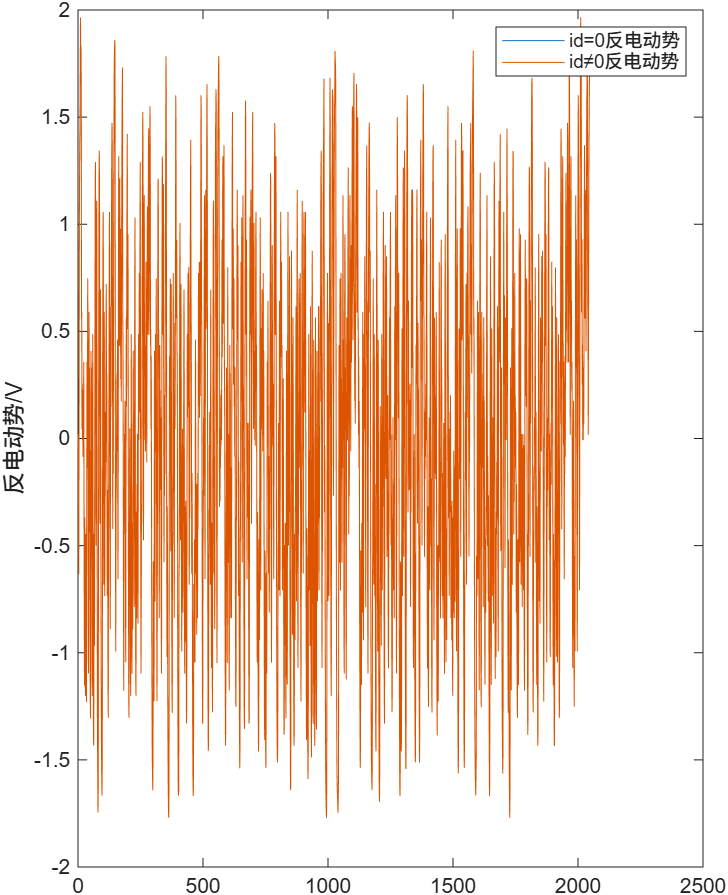
\includegraphics[width=\textwidth]
        {图片/速度环工作点2V反电动势对比.png}
        \caption{速度环工作点2V反电动势对比}
    \end{minipage}
    \begin{minipage}{0.5\textwidth}
        \centering
        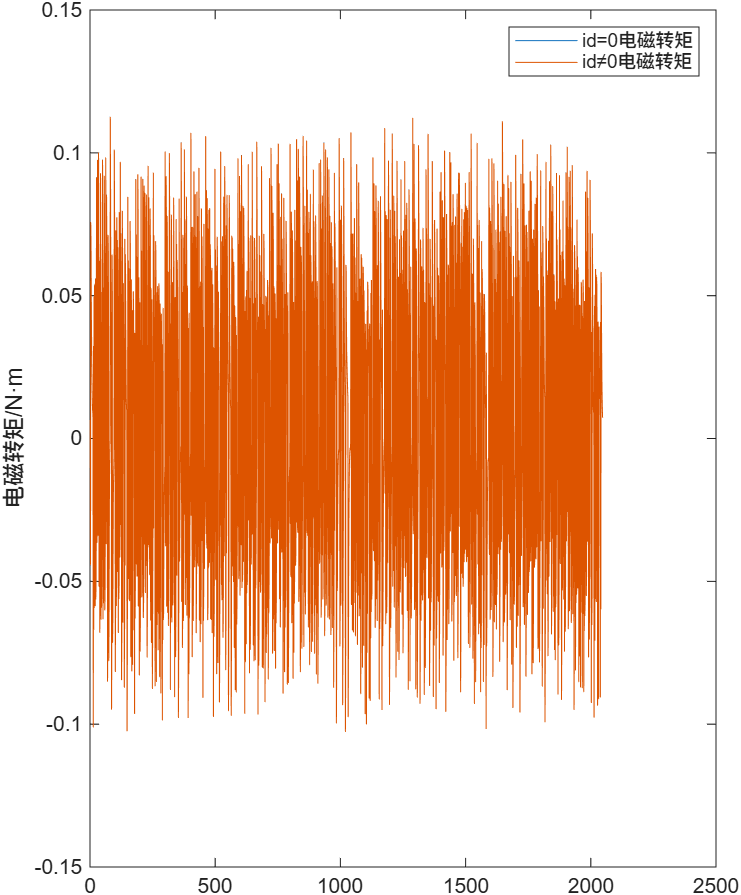
\includegraphics[width=\textwidth]
        {图片/速度环工作点2V电磁转矩对比.png}
        \caption{速度环工作点2V电磁转矩对比}
    \end{minipage}
    \label{fig:速度环工作点2V理想id与实际id对比}
\end{figure}

据上图可知，两者在反电动势和电磁转矩两条曲线上的差异均微乎其微，波形在时域上几乎完全重合。
为覆盖不同工作点下的情况，在\(U_{\mathrm{q}}=\pm2\text{V},\pm4\text{V}\)四个工作点均进行上述分析，
计算反电动势和电磁转矩在理想\(i_{\mathrm{d}}=0\)与实际\(i_{\mathrm{d}}\)下的相关系数与拟合优度，汇总如下表所示。
\begin{table}[H]
    \centering
    \begin{tabular}{|c|c|c|c|c|}
        \hline
        \multirow{2}{*}{工作点} & \multicolumn{2}{c|}{反电动势} & \multicolumn{2}{c|}{电磁转矩}\\
        \cline{2-5}
        & 相关系数 & 拟合优度 & 相关系数 & 拟合优度\\
        \hline
        \(U_{\mathrm{q}}=2\text{V}\) & 99.99991\% & 99.86604\% & 100.00000\% & 99.97521\%\\
        \hline
        \(U_{\mathrm{q}}=4\text{V}\) & 99.99987\% & 99.83449\% & 100.00000\% & 99.96860\%\\
        \hline
        \(U_{\mathrm{q}}=-2\text{V}\) & 99.99992\% & 99.86799\% & 100.00000\% & 99.97689\%\\
        \hline
        \(U_{\mathrm{q}}=-4\text{V}\) & 99.99985\% & 99.81871\% & 100.00000\% & 99.96570\%\\
        \hline
    \end{tabular}
    \caption{各工作点下\(i_{\mathrm{d}}=0\)理想假设与实测\(i_{\mathrm{d}}\)的差异评估}
    \label{tab:各工作点id=0假设验证汇总}
\end{table}

由表\ref{tab:各工作点id=0假设验证汇总}可知，四个工作点下的反电动势与电磁转矩的相关系数和
拟合优度均超过99.5\%，\(i_{\mathrm{d}}=0\)的简化假设在所有工作点下均完全成立。据此，可以确信后续基于
\(i_{\mathrm{d}}=0\)理想模型进行的间接法辨识及机械传递函数反推具备充分的工程合理性。

\subsubsection{不同工作点的机械部分传递函数辨识}
满足了\(i_{\mathrm{d}}=0\)的理想化近似条件后，才能真正开始基于间接法的机械传递函数辨识。
在\(U_{\mathrm{q}}=2V\)工作点附近给予伪随机激励，幅值2V，辨识从\(U_{\mathrm{q}}\)到\(n\)的传递函数，奇异值分解如下图所示和
数值解-解析解频域对比如下图所示。幅频相关系数99.08708\%，相频相关系数99.91204\%，复频率
拟合优度88.14769\%。根据奇异值分解图可得闭环传递函数应为2阶。辨识得到离散传递函数为：
\footnote{由于伪随机信号对直流增益几乎没有辨识能力，因此选取阶跃段的稳态值，除以激励值作为直流增益，
修正辨识结果。}
\(G(z)=\cfrac{195+1111z^{-1}}{60.17-51.9z^{-1}+12.32z^{-2}}\)。
\begin{figure}[H]
    \begin{minipage}{0.5\textwidth}
        \centering
        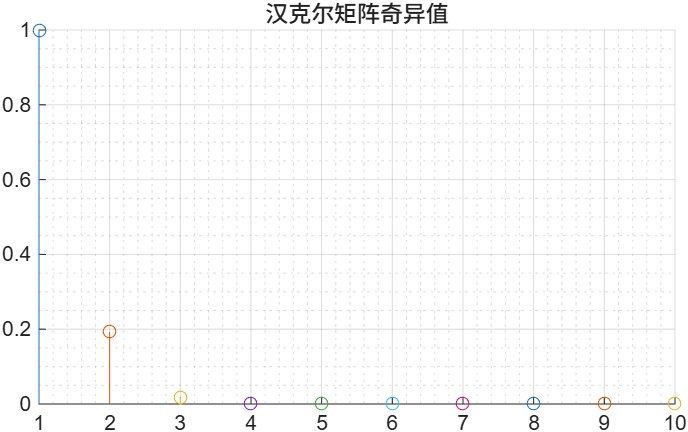
\includegraphics[width=\textwidth]
        {图片/速度环工作点2V奇异值分解图.jpg}
        \caption{速度环工作点2V奇异值分解图}
    \end{minipage}
    \begin{minipage}{0.5\textwidth}
        \centering
        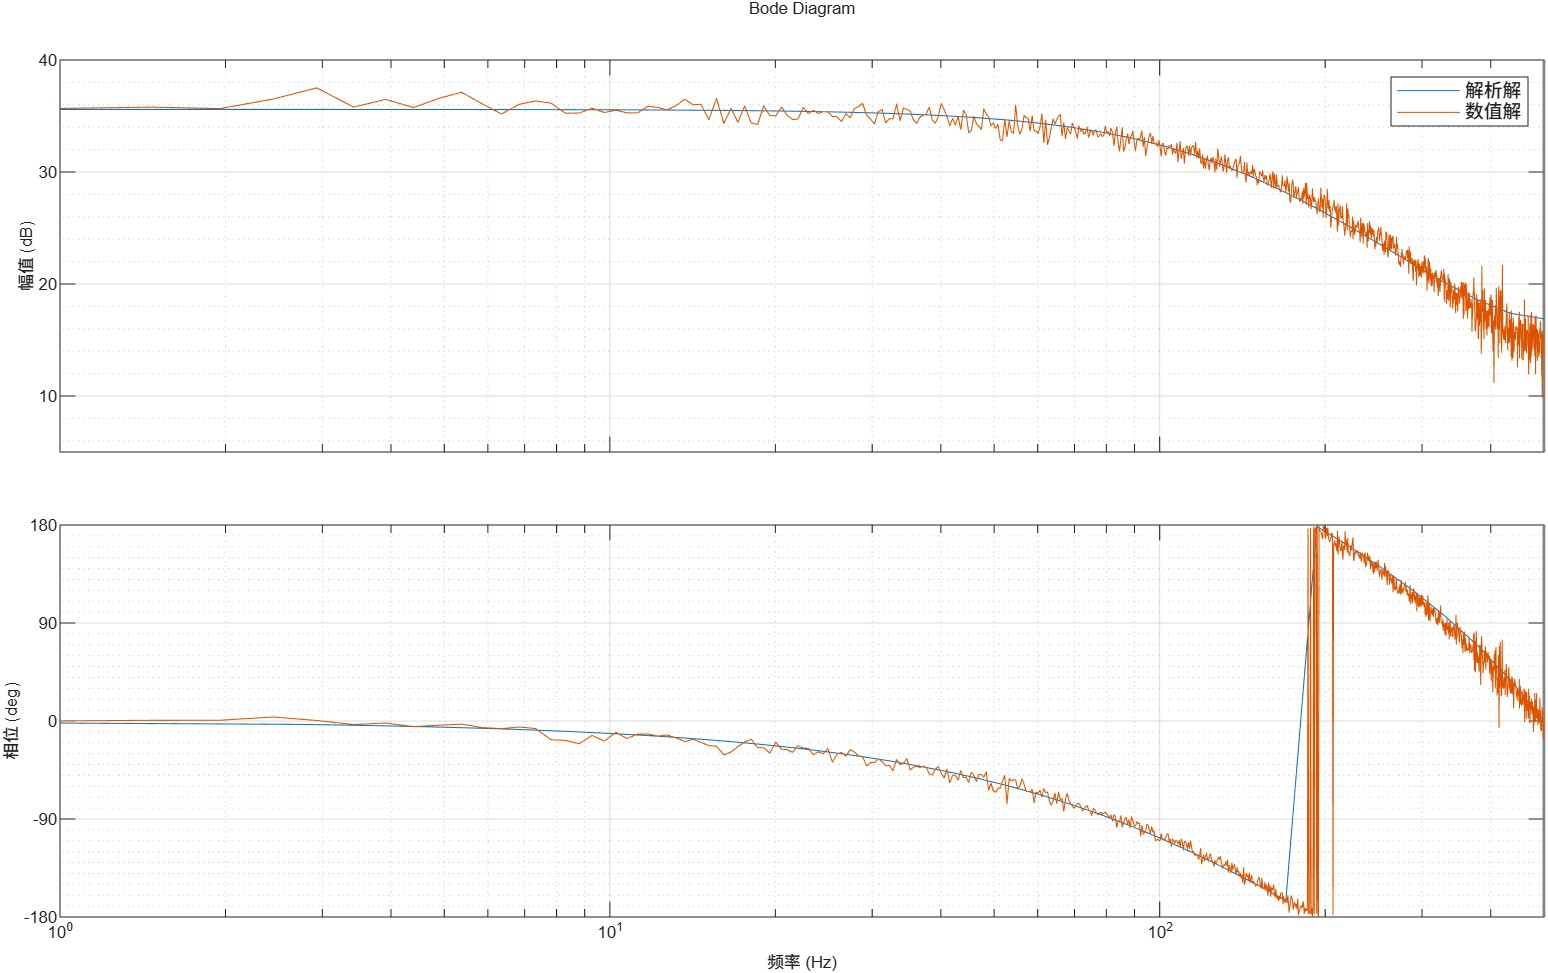
\includegraphics[width=\textwidth]
        {图片/速度环工作点2V数值解和解析解对比.jpg}
        \caption{速度环工作点2V数值解和解析解对比}
    \end{minipage}
\end{figure}

使用MATLAB的d2c命令，在零阶保持器ZOH作用下将辨识得到的闭环传递函数映射到连续域中，可得连续闭环传递函数
\(G(s)=\cfrac{-2.34\times 10^{4}s+4.578\times 10^7}{s^2+1586s+7.234\times 10^5}\)。根据图\ref{fig:Q轴电流-速度系统框图}
可知，闭环传递函数和机械部分的传递函数满足：
\begin{equation}
    G(s)=\cfrac{\cfrac{1}{R_{\mathrm{s}}+L_{\mathrm{q}}s}\times\cfrac{3}{2}p\psi_{\mathrm{m}}\times G_{\mathrm{m}}(s)}
    {1+\cfrac{1}{R_{\mathrm{s}}+L_{\mathrm{q}}s}\times\cfrac{3}{2}p\psi_{\mathrm{m}}\times G_{\mathrm{m}}(s)\times \cfrac{\pi}{30}p\psi_{\mathrm{m}}}
    \label{eq:Q轴电流-速度闭环传递函数表达式}
\end{equation}

推导可得：
\begin{equation}
    G_{\mathrm{m}}(s)=\cfrac{(R+L_{\mathrm{q}}s)G(s)}{\cfrac{3}{2}p\psi_{\mathrm{m}}[1-\cfrac{\pi}{30}p\psi_{\mathrm{m}}G(s)]}
    \label{eq:机械部分传递函数表达式}
\end{equation}

因此可得在2V工作点附近辨识得到的机械部分传递函数为
\begin{equation*}
    G_{\mathrm{m}}(s)=\cfrac{-50.76 s^4 - 1.145\times 10^5 s^3 + 1.709\times 10^8 s^2 + 
    3.901\times 10^{11} s + 1.892\times 10^{14}}
    {0.2028 s^4 + 710.2 s^3 + 7.781\times 10^{5} s^2 + 3.05\times 10^{8} s + 1.087\times 10^{10}}
\end{equation*}

机械部分传递函数看似为四阶，实际上为二阶，这是因为传递函数代数运算精度不足没能完全对消。求解上述传递函数的零极点结果为：
零点：[-2629.4、1959.4、-792.8±j307.9]；极点：[-1877.6、-792.8±j307.9、-39.5]。其中零点-792.8±j307.9和
极点-792.8±j307.9可以对消
\footnote{MATLAB显示精度问题，使得两个零极点看起来完全一致，实际上略有不同才导致没能完全抵消。但零极点的差异在该
数量级上可以忽略，视为对消}
。因此最终只剩下两个零点[-2629.4、1959.4]和
两个极点[-1877.6,-39.5]。而直流增益为[17398]。

后续其他工作点也按照上述方法进行，先辨识2阶的闭环传递函数，使用d2c命令在zoh选项下连续化得到连续域的闭环传递函数，
通过\eqref{eq:机械部分传递函数表达式}代数计算得到机械部分传递函数，将可以对消的零极点对消后按照两个零点、
两个极点和直流增益表征辨识结果。

工作点4V的闭环传递函数辨识结果如下图所示，幅频相关系数98.41397\%，相频相关系数99.79761\%，复频率
拟合优度83.84955\%。辨识得到离散传递函数为：\(G(z)=\cfrac{198.9+1150z^{-1}}{61.02-52.8z^{-1}+12.06z^{-2}}\)。
\begin{figure}[H]
    \begin{minipage}{0.5\textwidth}
        \centering
        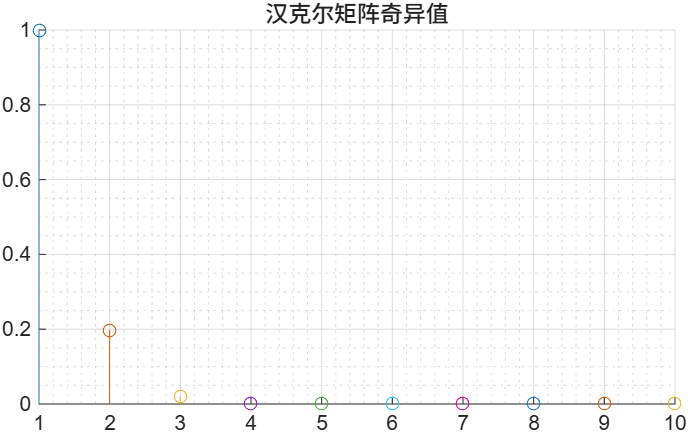
\includegraphics[width=\textwidth]
        {图片/速度环工作点4V奇异值分解图.png}
        \caption{速度环工作点4V奇异值分解图}
    \end{minipage}
    \begin{minipage}{0.5\textwidth}
        \centering
        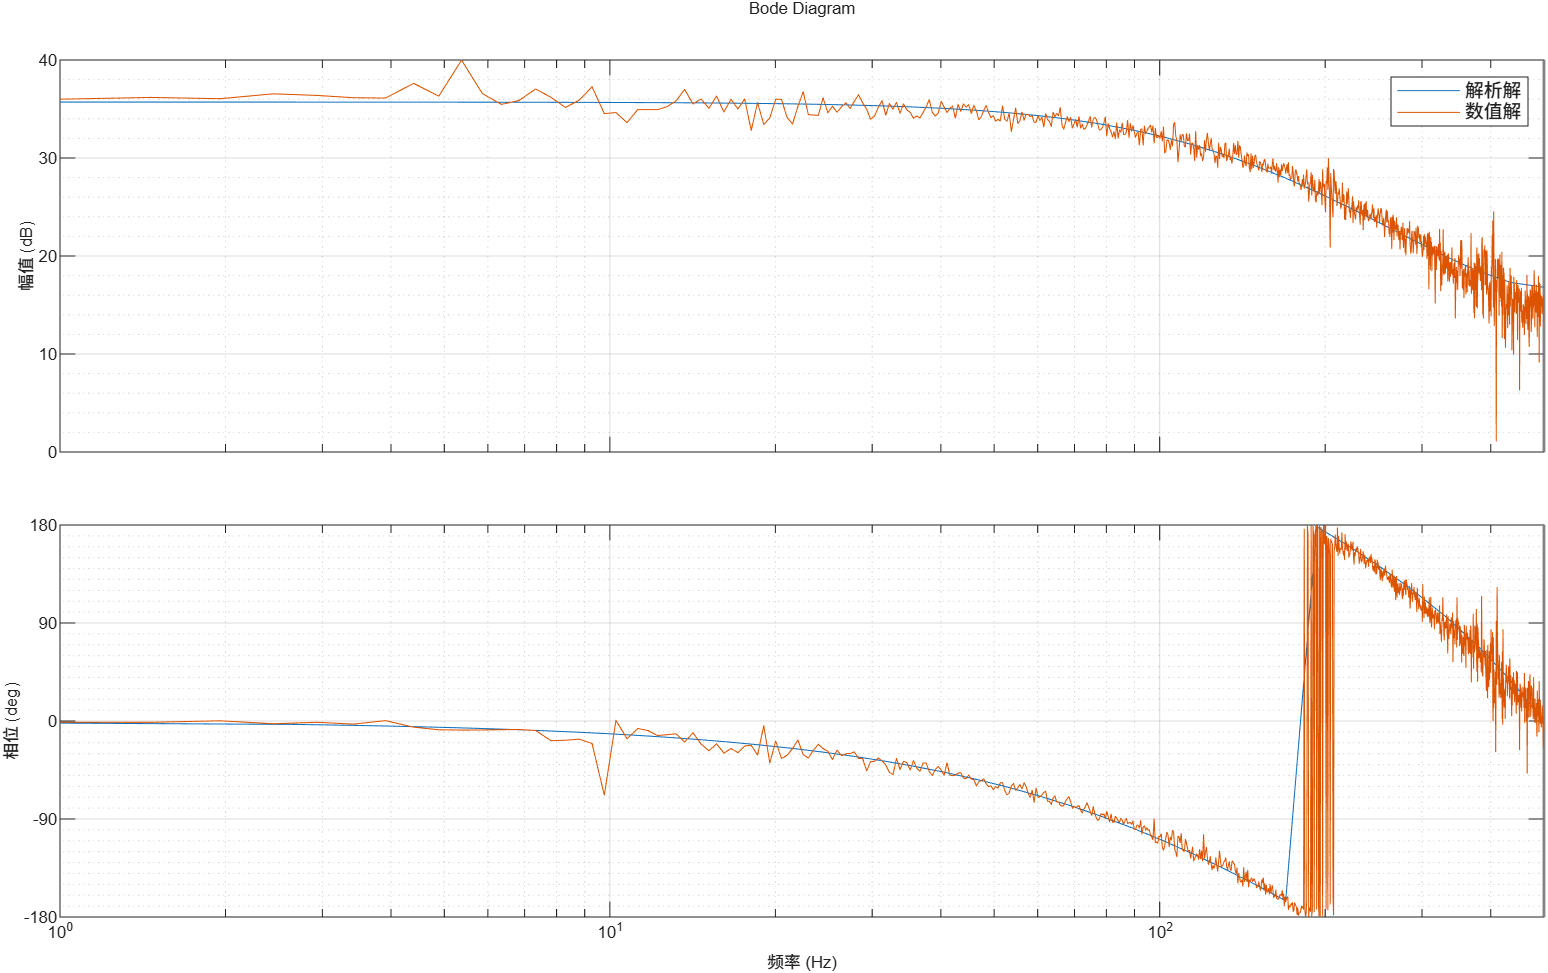
\includegraphics[width=\textwidth]
        {图片/速度环工作点4V数值解和解析解对比.png}
        \caption{速度环工作点4V数值解和解析解对比}
    \end{minipage}
\end{figure}
连续化、反推机械部分传递函数并消去零极点后得到零点[-2629.4,1943.5]和极点[-1945.1,-21]，直流增益[32510]
（零极点-810.7±j231.1对消）。

工作点-2V的闭环传递函数辨识结果如下图所示，幅频相关系数98.97118\%，相频相关系数99.91117\%，复频率
拟合优度87.59657\%。辨识得到离散传递函数为：\(G(z)=\cfrac{198.6+1126z^{-1}}{59.41-51.02z^{-1}+12.35z^{-2}}\)。
\begin{figure}[H]
    \begin{minipage}{0.5\textwidth}
        \centering
        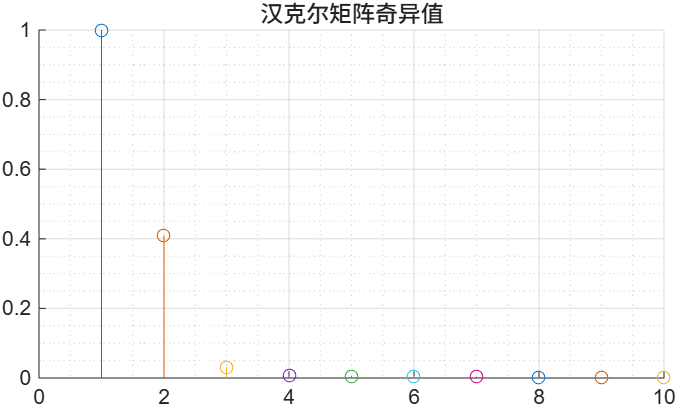
\includegraphics[width=\textwidth]
        {图片/速度环工作点-2V奇异值分解图.png}
        \caption{速度环工作点-2V奇异值分解图}
    \end{minipage}
    \begin{minipage}{0.5\textwidth}
        \centering
        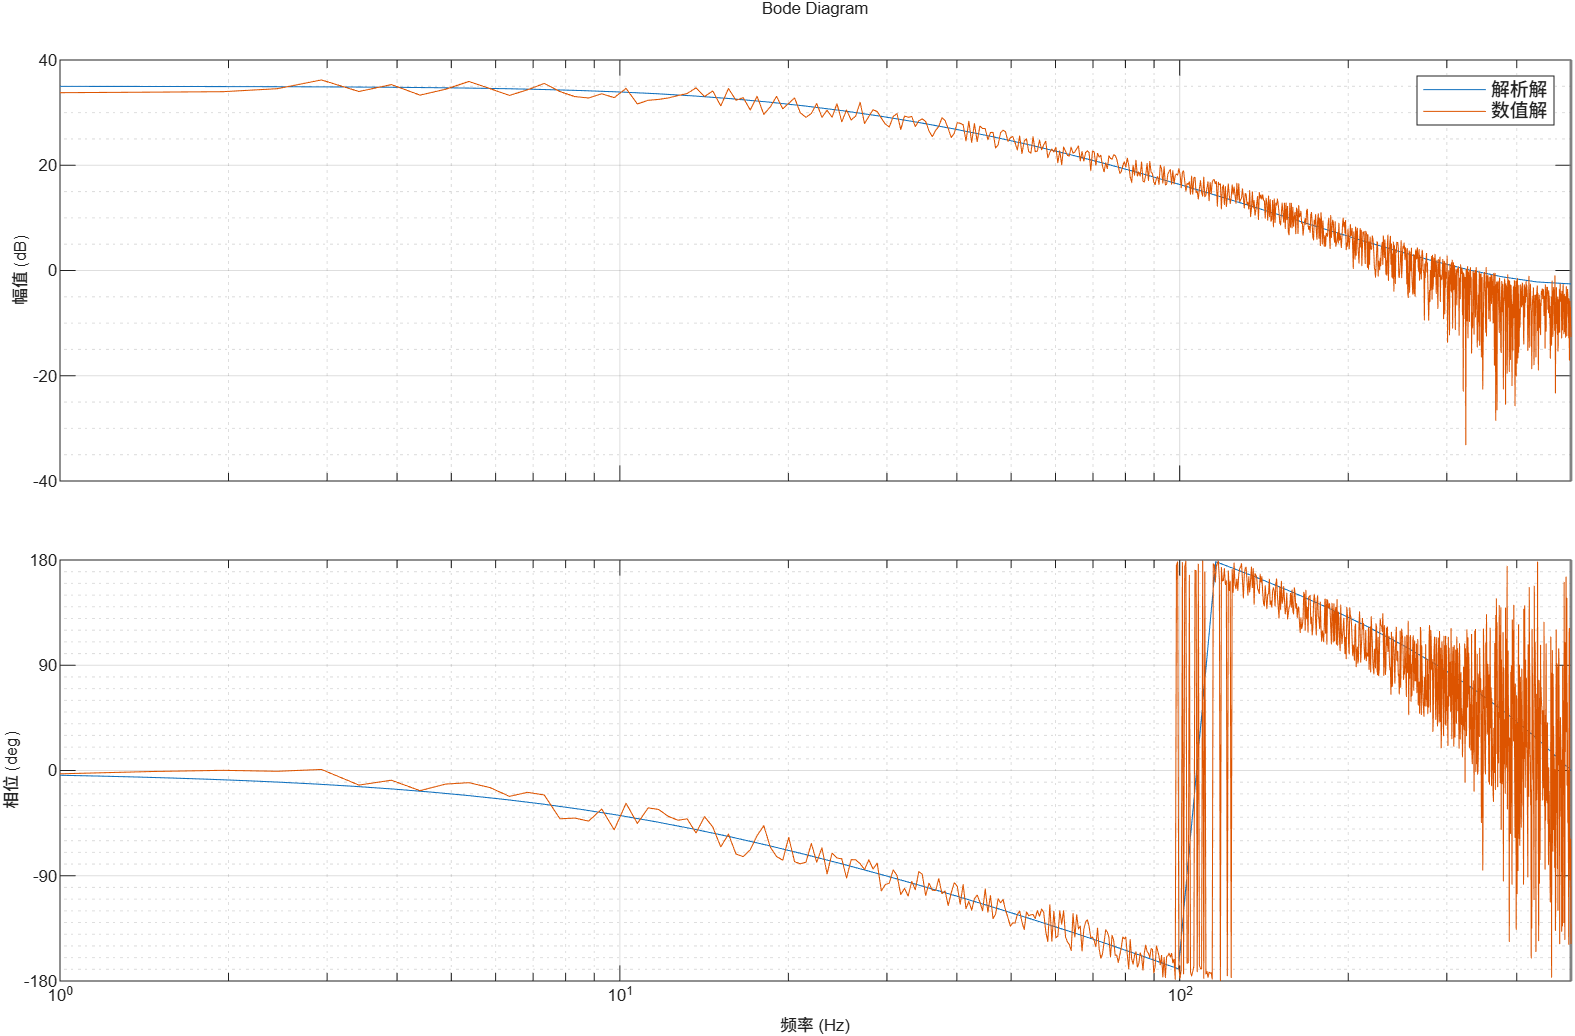
\includegraphics[width=\textwidth]
        {图片/速度环工作点-2V数值解和解析解对比.png}
        \caption{速度环工作点-2V数值解和解析解对比}
    \end{minipage}
\end{figure}
连续化、反推机械部分传递函数并消去零极点后得到零点[-2629.4,1964.2]和极点[-1870.7,-37.9]，直流增益[18622]
（零极点-785.3±j343.5对消）。

工作点-4V的闭环传递函数辨识结果如下图所示，幅频相关系数98.51759\%，相频相关系数99.76702\%，复频率
拟合优度84.81924\%。辨识得到离散传递函数为：\(G(z)=\cfrac{205.5+1146z^{-1}}{60.76-52.04z^{-1}+11.91z^{-2}}\)。
\begin{figure}[H]
    \begin{minipage}{0.5\textwidth}
        \centering
        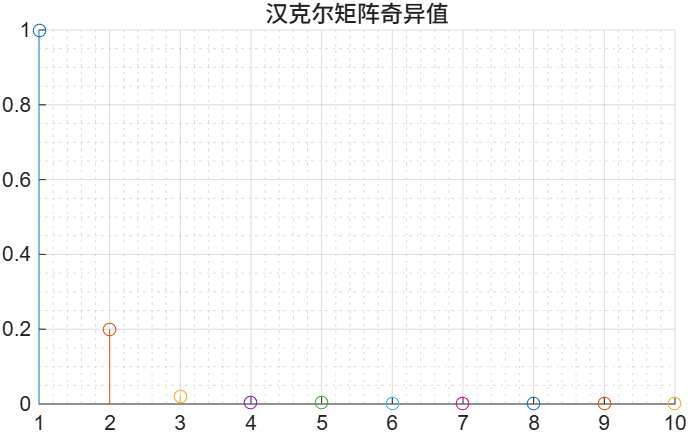
\includegraphics[width=\textwidth]
        {图片/速度环工作点-4V奇异值分解图.png}
        \caption{速度环工作点-4V奇异值分解图}
    \end{minipage}
    \begin{minipage}{0.5\textwidth}
        \centering
        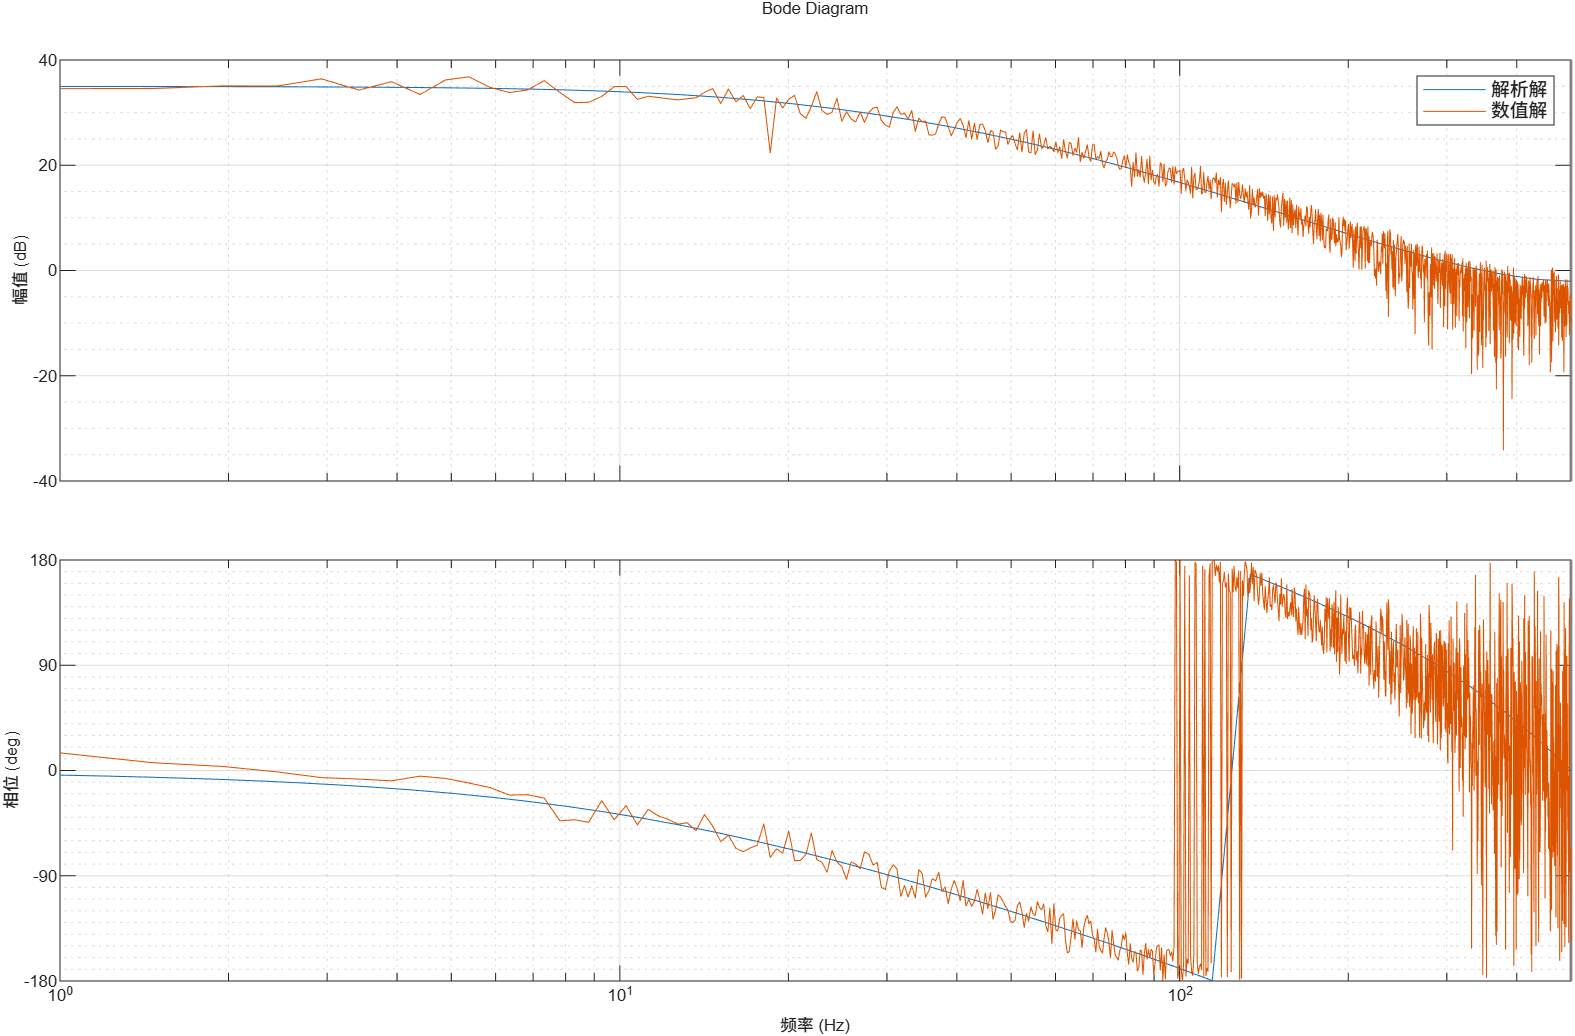
\includegraphics[width=\textwidth]
        {图片/速度环工作点-4V数值解和解析解对比.png}
        \caption{速度环工作点-4V数值解和解析解对比}
    \end{minipage}
\end{figure}
连续化、反推机械部分传递函数并消去零极点后得到零点[-2629.4,1956.0]和极点[-1948.7,-27.1]，直流增益[25478]
（零极点-814.9±j156.0对消）。

将上述四个工作点的机械部分传递函数辨识结果汇总如下表所示。
\begin{table}[H]
    \centering
    \begin{tabular}{|c|c|c|c|c|c|c|}
        \hline
        \multirow{2}{*}{工作点} & \multicolumn{3}{c|}{闭环辨识结果} & \multirow{2}{*}{极点} & \multirow{2}{*}{零点} & \multirow{2}{*}{直流增益} \\
        \cline{2-4}
        & 幅频相关系数 & 相频相关系数 & 拟合优度 & & & \\
        \hline
        \(U_{\mathrm{q}}=-4\text{V}\) & 98.51759\% & 99.76702\% & 84.81924\% & -1948.7, -27.1 & -2629.4, 1956.0 & 25478\\
        \hline
        \(U_{\mathrm{q}}=-2\text{V}\) & 98.97118\% & 99.91117\% & 87.59657\% & -1870.7, -37.9 & -2629.4, 1964.2 & 18622\\
        \hline
        \(U_{\mathrm{q}}=2\text{V}\)  & 99.08708\% & 99.91204\% & 88.14769\% & -1877.6, -39.5 & -2629.4, 1959.4 & 17398\\
        \hline
        \(U_{\mathrm{q}}=4\text{V}\)  & 98.41397\% & 99.79761\% & 83.84955\% & -1945.1, -21.0  & -2629.4, 1943.5 & 32510\\
        \hline
    \end{tabular}
    \caption{各工作点机械部分传递函数\(G_{\mathrm{m}}(s)\)辨识结果汇总}
    \label{tab:各工作点Gm辨识结果汇总}
\end{table}

\subsubsection{反推结果的敏感性分析与辨识模型求解\label{sec:反推结果的敏感性分析}}
实际工程上使用上述方法时，依赖于已经完成辨识的参数的精确度，若已完成辨识的参数误差较大，会导致辨识的机械传递函数
\(G_{\mathrm{m}}(s)\)偏差严重，接下来对此进行简单分析，并说明如何从表\ref{tab:各工作点Gm辨识结果汇总}中
得到较为合适的辨识模型。

反推式\eqref{eq:机械部分传递函数表达式}可改写为乘除结构：
\begin{equation*}
    G_{\mathrm{m}}(s)=\cfrac{R_{\mathrm{s}}+L_{\mathrm{q}}s}{\cfrac{3}{2}p\psi_{\mathrm{m}}}\times G(s)\times\cfrac{1}{1-\cfrac{\pi}{30}p\psi_{\mathrm{m}}G(s)}
\end{equation*}

其中\(R_{\mathrm{s}}\)、\(L_{\mathrm{q}}\)、\(\psi_{\mathrm{m}}\)与辨识得到的\(G(s)\)均存在误差
\footnote{相电阻\(R_{\mathrm{s}}\)、Q轴同步电感\(L_{\mathrm{q}}\)和永磁体磁链\(\psi_{\mathrm{m}}\)为常数，其误差是绝对误差；
闭环传递函数\(G(s)\)的误差指不同频点下复数误差的大小（含幅值与相位）。}。
对上式取对数可得：
\begin{equation*}
    \ln G_{\mathrm{m}}(s)=\ln(R_{\mathrm{s}}+L_{\mathrm{q}}s)+\ln G(s)-\ln\cfrac{3}{2}p\psi_{\mathrm{m}}-\ln[1-\cfrac{\pi}{30}p\psi_{\mathrm{m}}G(s)]
\end{equation*}

那么相对误差的传播公式就是一节全微分的形式：
\begin{align*}
    \cfrac{\Delta G_{\mathrm{m}}(s)}{G_{\mathrm{m}}(s)}&=
    \cfrac{\Delta[R_{\mathrm{s}}+L_{\mathrm{q}}s]}{R_{\mathrm{s}}+L_{\mathrm{q}}s}
    +\cfrac{\Delta G(s)}{G(s)}-\cfrac{\Delta(\cfrac{3}{2}p\psi_{\mathrm{m}})}{\cfrac{3}{2}p\psi_{\mathrm{m}}}
    +\cfrac{\Delta[1-\cfrac{\pi}{30}p\psi_{\mathrm{m}}G(s)]}{1-\cfrac{\pi}{30}p\psi_{\mathrm{m}}G(s)}\\
    &=\cfrac{\Delta R_{\mathrm{s}}+s\Delta L_{\mathrm{q}}}{R_{\mathrm{s}}+L_{\mathrm{q}}s}+
    \cfrac{\Delta G(s)}{G(s)}-\cfrac{\Delta \psi_{\mathrm{m}}}{\psi_{\mathrm{m}}}-
    (-\cfrac{\cfrac{\pi}{30}pG(s)\Delta\psi_{\mathrm{m}}}{1-\cfrac{\pi}{30}p\psi_{\mathrm{m}}G(s)}
    -\cfrac{\cfrac{\pi}{30}p\psi_{\mathrm{m}}\Delta G(s)}{1-\cfrac{\pi}{30}p\psi_{\mathrm{m}}G(s)})\\
    &=\cfrac{R_{\mathrm{s}}}{R_{\mathrm{s}}+s L_{\mathrm{q}}}\cfrac{\Delta R_{\mathrm{s}}}{R_{\mathrm{s}}}+
    \cfrac{s L_{\mathrm{q}}}{R_{\mathrm{s}}+s L_{\mathrm{q}}}\cfrac{\Delta L_{\mathrm{q}}}{L_{\mathrm{q}}}+
    \cfrac{1}{1-\cfrac{\pi}{30}p\psi_{\mathrm{m}}G(s)}\cfrac{\Delta G(s)}{G(s)}+
    \cfrac{\cfrac{\pi}{15}p\psi_{\mathrm{m}}G(s)-1}{1-\cfrac{\pi}{30}p\psi_{\mathrm{m}}G(s)}\cfrac{\Delta\psi_{\mathrm{m}}}{\psi_{\mathrm{m}}}
\end{align*}

定义灵敏度函数：
\begin{equation}
    \begin{cases}
        S_{R}(\mathrm{j}\omega)=\cfrac{R_{\mathrm{s}}}{R_{\mathrm{s}}+\mathrm{j}\omega L_{\mathrm{q}}}\\
        S_{L}(\mathrm{j}\omega)=\cfrac{\mathrm{j}\omega L_{\mathrm{q}}}{R_{\mathrm{s}}+\mathrm{j}\omega L_{\mathrm{q}}}\\
        S_{G}(\mathrm{j}\omega)=\cfrac{1}{1-\cfrac{\pi}{30}p\psi_{\mathrm{m}}G(\mathrm{j}\omega)}\\
        S_{\psi}(\mathrm{j}\omega)=\cfrac{\cfrac{\pi}{15}p\psi_{\mathrm{m}}G(\mathrm{j}\omega)-1}{1-\cfrac{\pi}{30}p\psi_{\mathrm{m}}G(\mathrm{j}\omega)}
    \end{cases}
    \label{eq:灵敏度函数}
\end{equation}

那么相对误差可以表示为：
\begin{equation*}
    \cfrac{\Delta G_{\mathrm{m}}(\mathrm{j}\omega)}{G_{\mathrm{m}}(\mathrm{j}\omega)}=
    S_{R}(\mathrm{j}\omega)\cfrac{\Delta R_{\mathrm{s}}}{R_{\mathrm{s}}}
    +S_{L}(\mathrm{j}\omega)\cfrac{\Delta L_{\mathrm{q}}}{L_{\mathrm{q}}}
    +S_{G}(\mathrm{j}\omega)\cfrac{\Delta G}{G(s)}
    +S_{\psi}(\mathrm{j}\omega)\cfrac{\Delta \psi_{\mathrm{m}}}{\psi_{\mathrm{m}}}
\end{equation*}

由于\(\psi_{\mathrm{m}}\)的辨识依赖于\(R_{\mathrm{s}}\)，\(L_{\mathrm{q}}\)的辨识依赖于\(R_{\mathrm{s}}\)与
\(\psi_{\mathrm{m}}\)，各输入量的误差经误差传递相互关联，并非独立，无法按独立误差作均方根合成。
因此取最坏情况下的线性叠加，作为反推结果相对标准差的上界：
\begin{equation}
    \cfrac{\sigma_{G_{\mathrm{m}}}(\omega)}{|G_{\mathrm{m}}(\mathrm{j}\omega)|}
    =|S_R(\mathrm{j}\omega)|\cfrac{\sigma_R}{R_{\mathrm{s}}}
    +|S_L(\mathrm{j}\omega)|\cfrac{\sigma_L}{L_{\mathrm{q}}}
    +|S_G(\mathrm{j}\omega)|\cfrac{\sigma_G(\omega)}{|G(\mathrm{j}\omega)|}
    +|S_\psi(\mathrm{j}\omega)|\cfrac{\sigma_\psi}{\psi_{\mathrm{m}}}
    \label{eq:标准差上界}
\end{equation}

其中\(\sigma_R,\sigma_L,\sigma_\psi\)分别为\(R_{\mathrm{s}},L_{\mathrm{q}},\psi_{\mathrm{m}}\)的标准差
，根据前文数据可得相对标准误差分别为：\(\cfrac{\sigma_R}{R_{\mathrm{s}}}=2.78\%\)、\(\cfrac{\sigma_L}{L_{\mathrm{q}}}=0.2\%\)
\footnote{简单起见，\(L_{\mathrm{q}}\)的相对标准误差采用相间电感测量时得到的值。}、
\(\cfrac{\sigma_\psi}{\psi_{\mathrm{m}}}=1.79\%\)。而
\(\cfrac{\sigma_G(\omega)}{|G(\mathrm{j}\omega)|}\)为闭环辨识的相对误差，由相干函数按\eqref{eq:估计方差与相干函数}估计。

对四个工作点分别计算上式，得到反推结果相对标准误差随频率的分布，结果如下图所示。
\begin{figure}[H]
    \begin{minipage}{0.5\textwidth}
        \centering
        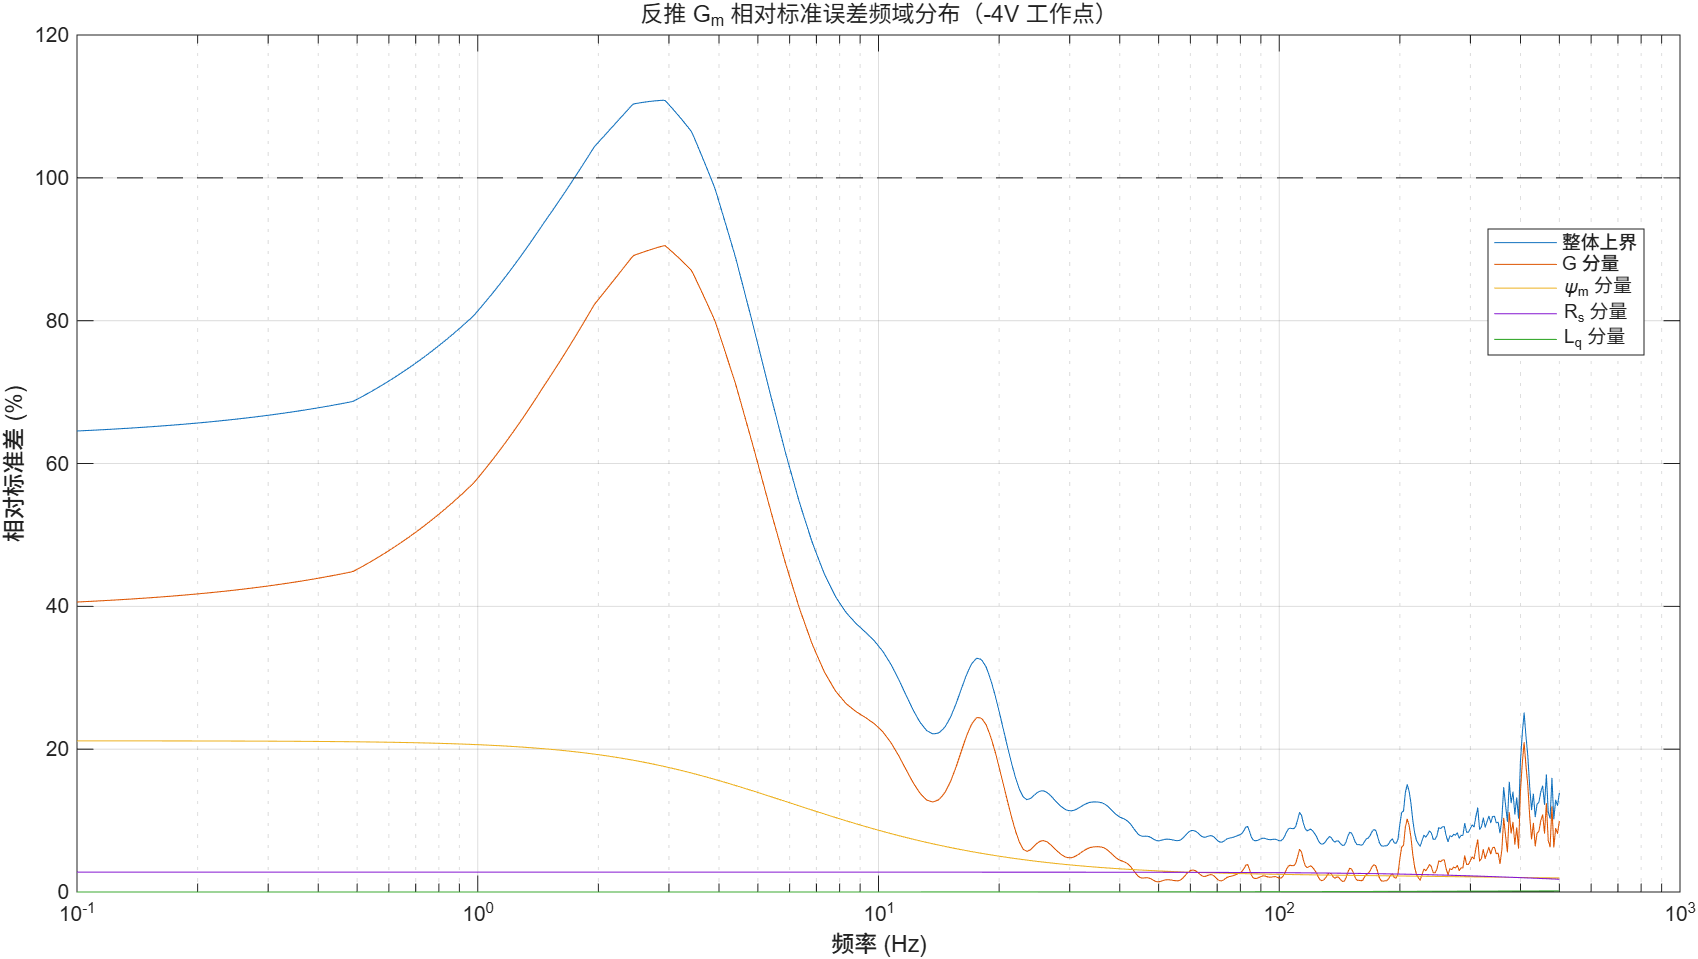
\includegraphics[width=\textwidth]
        {图片/相对标准误差频域分布曲线（-4V）.png}
        \caption{相对标准误差频域分布曲线（-4V）}
        \label{fig:相对标准误差频域分布曲线（-4V）}
    \end{minipage}
    \begin{minipage}{0.5\textwidth}
        \centering
        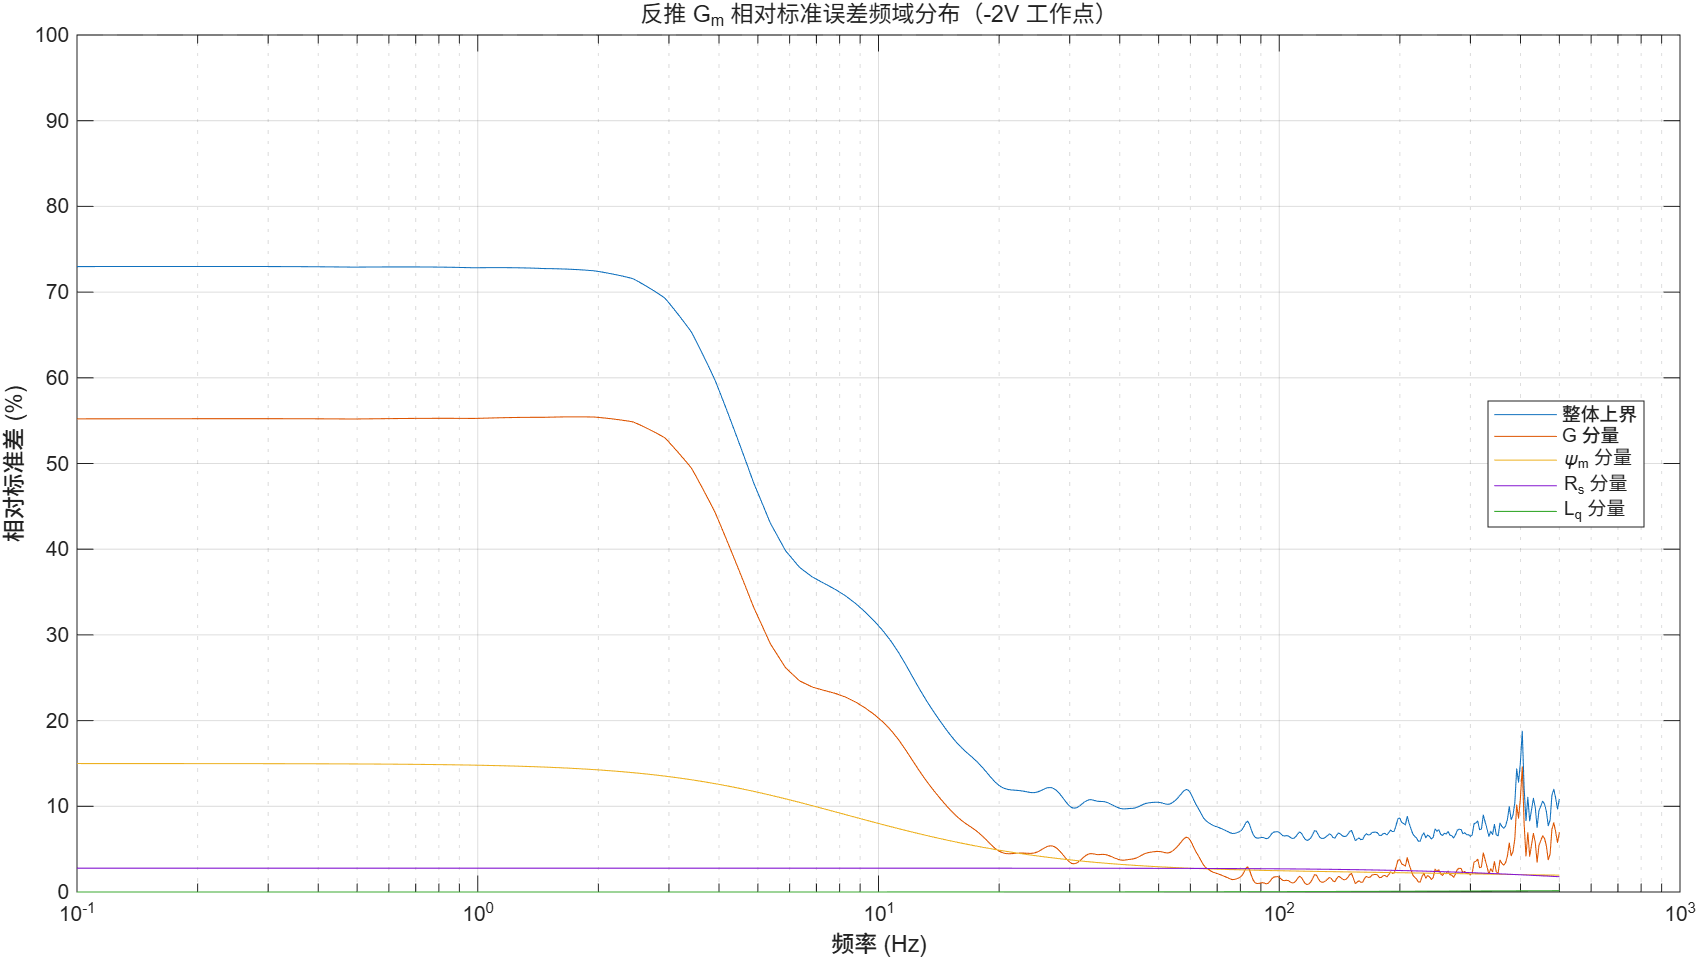
\includegraphics[width=\textwidth]
        {图片/相对标准误差频域分布曲线（-2V）.png}
        \caption{相对标准误差频域分布曲线（-2V）}
        \label{fig:相对标准误差频域分布曲线（-2V）}
    \end{minipage}
\end{figure}
\begin{figure}[H]
    \begin{minipage}{0.5\textwidth}
        \centering
        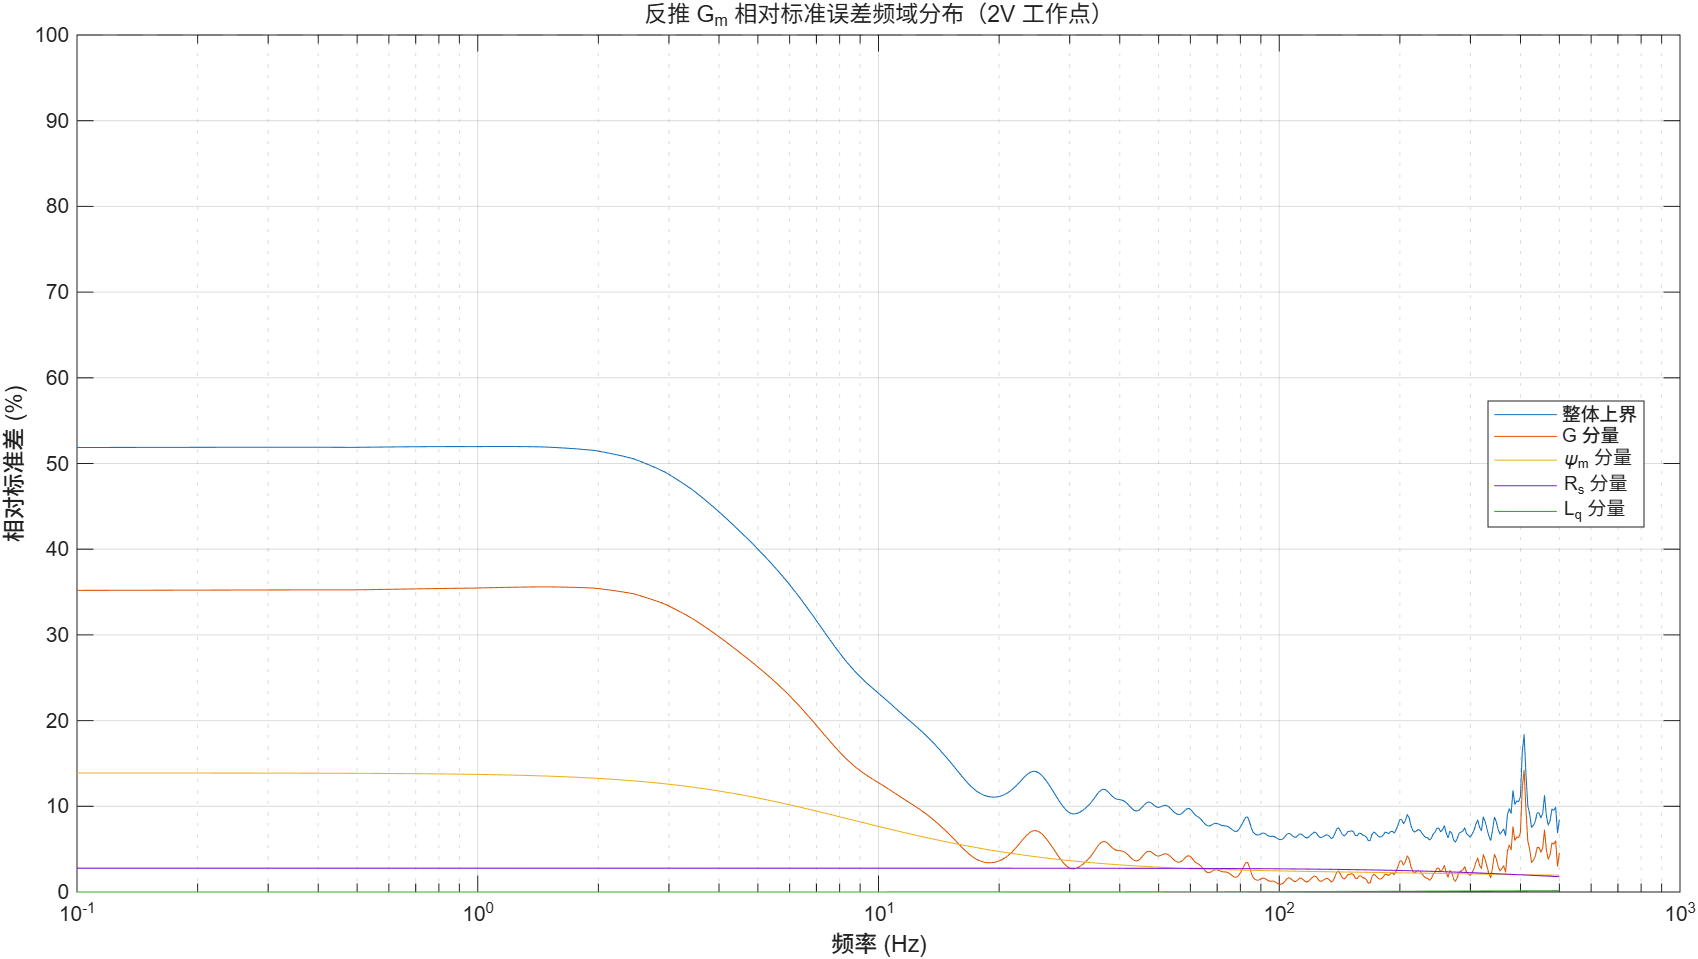
\includegraphics[width=\textwidth]
        {图片/相对标准误差频域分布曲线（2V）.png}
        \caption{相对标准误差频域分布曲线（2V）}
        \label{fig:相对标准误差频域分布曲线（2V）}
    \end{minipage}
    \begin{minipage}{0.5\textwidth}
        \centering
        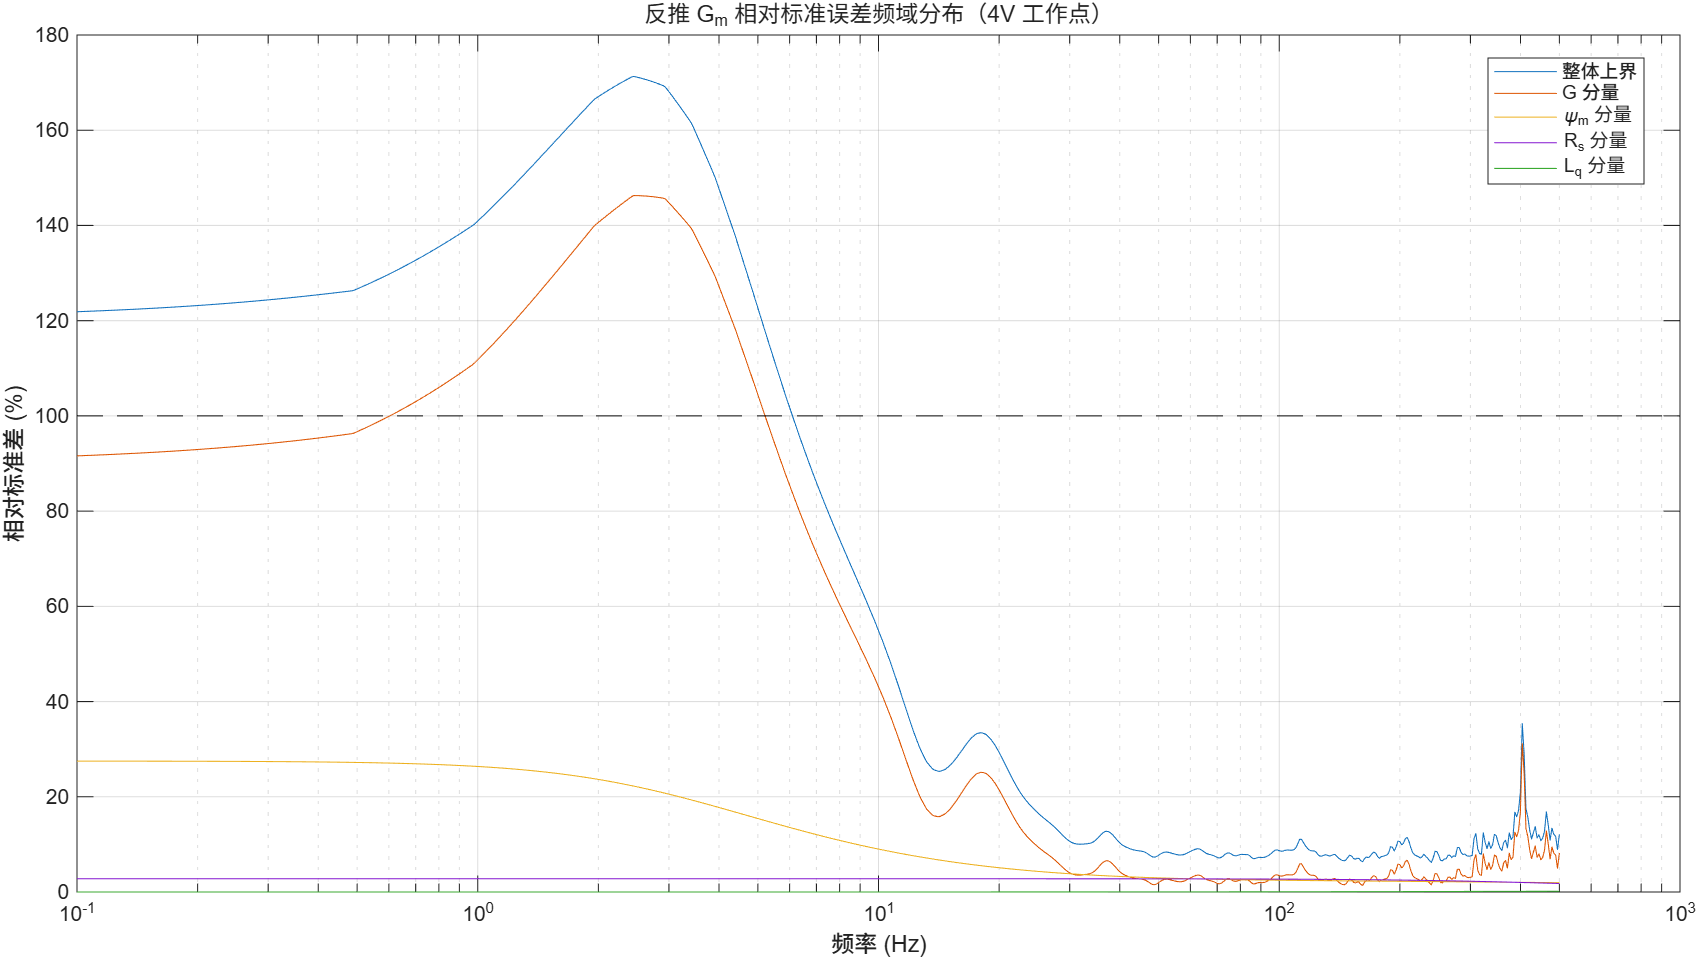
\includegraphics[width=\textwidth]
        {图片/相对标准误差频域分布曲线（4V）.png}
        \caption{相对标准误差频域分布曲线（4V）}
        \label{fig:相对标准误差频域分布曲线（4V）}
    \end{minipage}
\end{figure}

由图可知，±4V工作点在低频的相对误差超过100\%，即该处反推得到的\(G_{\mathrm{m}}\)误差已超过其本身，结果不可信；
±2V工作点相对误差均在75\%以下，其中核心频段（\(10\text{Hz}\sim 100\text{Hz}\)）约为20\%\(\sim\)30\%。
且±2V的误差随频率升高而降低，±4V在低频出现明显的破百峰。这解释了表\ref{tab:各工作点Gm辨识结果汇总}
中±4V工作点结果散布更大、而±2V工作点结果更一致的现象。据此，选取±2V工作点的平均结果作为参考模型，
排除反推结果不可信的±4V工作点。

最终得到极点[-1874.2, -38.7]、零点[-2629.4, 1961.8]、直流增益[18010]的机械传递函数：
\begin{equation}
    G_{\mathrm{m}}(s) = \frac{-18010s^2 - 1.202\times 10^7 s + 9.29\times 10^{10}}
    {71.12s^2 + 1.36\times 10^5 s + 5.158\times 10^6}
    \label{eq:Gm参考模型}
\end{equation}

值得说明的是，极低频段的辨识误差对闭环控制性能的影响较为有限，这是因为为了实现无差跟踪控制器含积分环节，
低频时开环增益趋于无穷，闭环传递函数在低频趋于1，因此辨识模型的低频辨识误差能够被控制器压制。
真正影响控制器设计的是核心频段10\(\sim\)100Hz的误差，该频段±2V工作点的相对误差为
20\%\(\sim\)30\%，还可以通过增大裕度来压制。±4V工作点在这部分的相对误差更高，故采用±2V工作点的辨识结果。

另外，如果想要较为准确地获取极低频段的辨识结果（主要是开环直流增益），可以尝试通过多点闭环直流增益（转速常数）测量，拟合出平均
闭环直流增益直接反推开环直流增益。实测发现，闭环直流增益最小二乘拟合后约67.4 rpm/V，
高于辨识模型隐含的约63.6 rpm/V，且观察到了明显的转速常数随工作点而升高的现象。
将修正后的开环直流增益代入模型后，开环与闭环验证均与实测明显不符。
推测原因有三个：其一是灵敏度函数\(S_{G}(\mathrm{j\omega})\)太大，转速常数的很小偏差都会在开环直流增益中引发
极大的偏离\footnote{直流处灵敏度函数\(S_G(\mathrm{j}0)=[1-\cfrac{\pi}{30}p\psi_{\mathrm{m}}G(0)]^{-1}\approx 22\)，
即转速常数（闭环直流增益）1\%的相对偏差经反推会被放大为开环直流增益约22\%的偏离。}；其二是电机本身的非线性因素较强，齿槽转矩严重，
在恒定电压激励下会因为齿槽转矩而发生周期性波动，难以准确计算
稳态转速和转速常数；其三是由于机械摩擦和逆变器死区导致测得的转速常数随激励电压而变化，使得用单一数值描述本身就缺乏合理性。
最终确定开环直流增益无法由闭环数据稳健反推，故保留辨识模型，并将极低频误差交由积分环节压制。

\subsubsection{辨识结果的开环验证}
根据\eqref{eq:Q轴电流-速度闭环传递函数表达式}，可以得到Q轴反电动势闭环传递函数：
\begin{equation*}
    G(s)=\cfrac{-3774 s^2 - 2.068\times10^6 s + 2.065\times 10^{10}}
    {2.298 s^3 + 7367 s^2 + 3.607\times 10^6 s +3.238\times 10^{8}}
\end{equation*}

由于电机的速度来源与对角度传感器的微分，微分噪声极大，因此在开环和后续的闭环验证中需要加入低通滤波器
\(F(z)=\cfrac{0.1}{1-0.9z^{-1}}\)
\footnote{辨识时不加入该滤波器，主要出于两方面考虑。其一，滤波器串联后辨识得到的是\(F(z)\times\text{ZOH}[G_{\mathrm{m}}(s)]\)的级联模型，
从中分离\(G_{\mathrm{m}}(s)\)需进行反卷积，会引入额外不确定性。其二，\(F(z)\)的极点\(z=0.9\)对应连续域频率远高于机械带宽，
Ho-Kalman辨识算法试图在全频段进行拟合，需分配额外阶次拟合该快动态，在有限数据长度下会削弱机械模态的估计精度。实测结果也表明，
加入\(F(z)\)尽管转速信号更加平滑，但辨识的拟合优度和幅相频相关系数均有下降，模型与实测波形的吻合程度也不及不加滤波器时。
因此采用分步策略——辨识时直接获取\(G_{\mathrm{m}}(s)\)，验证时在输出端串联\(F(z)\)实现物理模型与测量滤波的解耦。}。
此时系统框图变为：
\begin{figure}[H]
    \centering
    \begin{tikzpicture}[auto, node distance=2cm, >=latex']
        % 样式定义
        \tikzstyle{block} = [draw, rectangle, minimum height=3em, minimum width=1.5em, align=center]
        \tikzstyle{sum} = [draw, circle, node distance=1.5cm, minimum size=0.5em, inner sep=0pt]
        \tikzstyle{input} = [coordinate]
        \tikzstyle{output} = [coordinate]
        \tikzstyle{feedback} = [coordinate]

        % 放置节点
        \node [input, name=input] {};
        \node [sum, right of=input] (sum) {};
        \node [block, right of=sum] (RL) {\(\cfrac{1}{R_{\mathrm{s}}+L_{\mathrm{q}} s}\)};
        \node [block, right of=RL] (K) {\(\cfrac{3}{2}p\psi_{\mathrm{m}}\)};
        \node [block, right of=K] (Mech) {\(G_{\mathrm{m}}(s)\)};
        \node [block, right of=Mech] (ZOH) {ZOH};
        \node [block, right of=ZOH] (F) {\(F(z)\)};
        \node [output, right of=F] (output) {};
        \node [block, below of=K, node distance=1.5cm] (Kf) {\(\cfrac{\pi}{30}p\psi_{\mathrm{m}}\)};

        \draw [->] (input) -- node {\(U_{\mathrm{q}}\)} (sum);
        \draw [->] (sum) -- node {\(U_{\mathrm{q}}'\)} (RL);
        \draw [->] (RL) -- node {\(i_{\mathrm{q}}\)} (K);
        \draw [->] (K) -- node {\(T_{\mathrm{e}}\)} (Mech);
        \draw [->] (Mech) -- node [name=y] {\(n\)} (ZOH);
        \draw [->] (ZOH) -- node {} (F);
        \draw [->] (F) -- node {\(n_{\mathrm{fi}}\)} (output);
        \draw [->] (y) |- (Kf);
        \draw [->] (Kf) -| node[pos=0.9] {\(-\)} node [pos=0.5] {\(E\)} (sum);
    \end{tikzpicture}
    \caption{\(i_{\mathrm{d}}=0\)假设下的Q轴电流-速度系统框图（带低通滤波器）}
    \label{fig:Q轴电流-速度系统框图（带低通滤波器）}
\end{figure}

因此实际闭环传递函数应为使用零阶保持器离散化后与离散低通滤波器\(F(z)\)相乘的结果：
\begin{equation*}
    G(z)=\cfrac{0.3297 z^{-1} + 1.85 z^{-2} - 0.1351 z^{-3}}
    {1- 1.832 z^{-1} + 1.108 z^{-2} - 0.2565z^ {-3} + 0.0134z^{-4}}
\end{equation*}

选用幅值为±5V的方波信号作为激励信号，输入到\(U_{\mathrm{q}}\)，同时进行D轴闭环\(i_{\mathrm{d}}^*=0\)，在电机空载的情况下记录电机的转速响应。
但首先仍需要考虑\(i_{\mathrm{d}}=0\)理想条件是否满足。

施加正向方波时，考虑\(i_{\mathrm{d}}=0\)的理想化假设和\(i_{\mathrm{d}}\ne 0\)的实际情况，分析反电动势和电磁转矩波形如下图所示。
\begin{figure}[H]
    \begin{minipage}{0.5\textwidth}
        \centering
        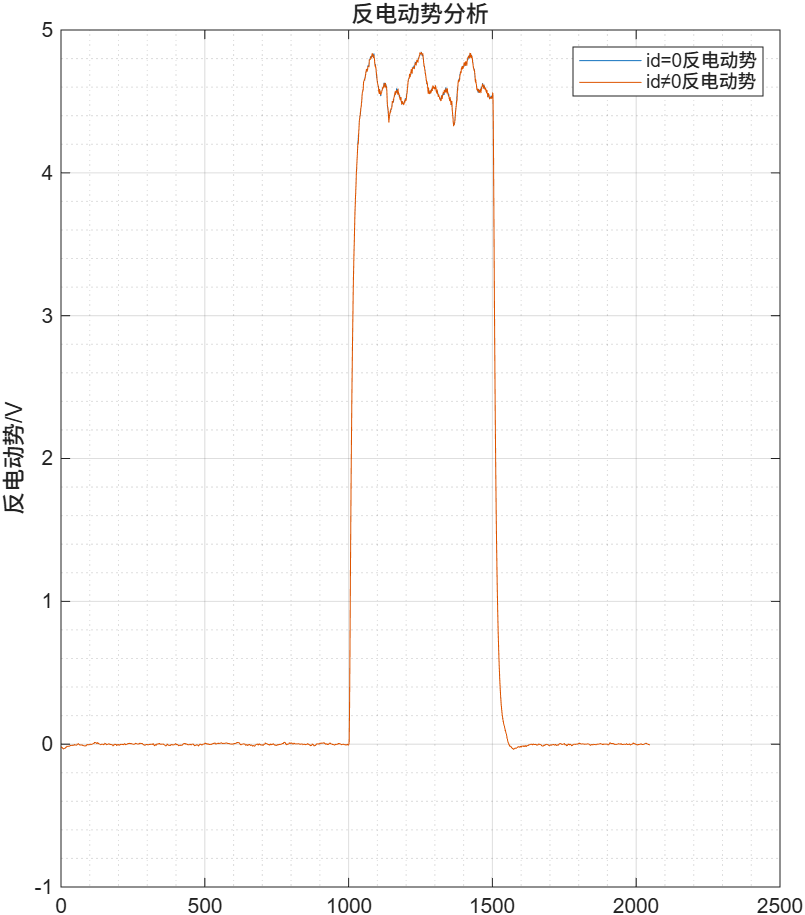
\includegraphics[width=\textwidth]  
        {图片/速度环正向方波反电动势对比.png}
        \caption{速度环正向方波反电动势对比}
    \end{minipage}
    \begin{minipage}{0.5\textwidth}
        \centering
        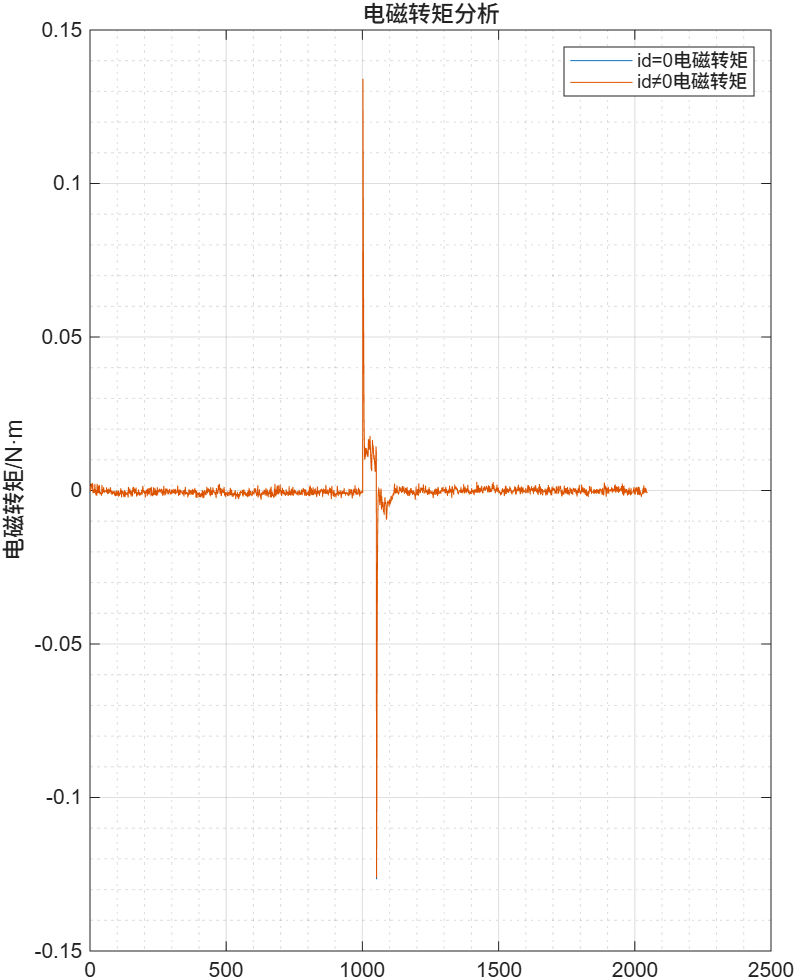
\includegraphics[width=\textwidth]
        {图片/速度环正向方波电磁转矩对比.png}
        \caption{速度环正向方波电磁转矩对比}
    \end{minipage}
    \label{fig:速度环正向方波理想id与实际id对比}
\end{figure}

分析可得反电动势相关系数99.99988\%，拟合优度99.84557\%；电磁转矩相关系数100.00000\%，拟合优度99.97289\%为极高水平，\(i_{\mathrm{d}}=0\)的
理想化假设可以认为是遵守的。此时仿真和实测的转速波形如下图所示。
\begin{figure}[H]
    \centering
    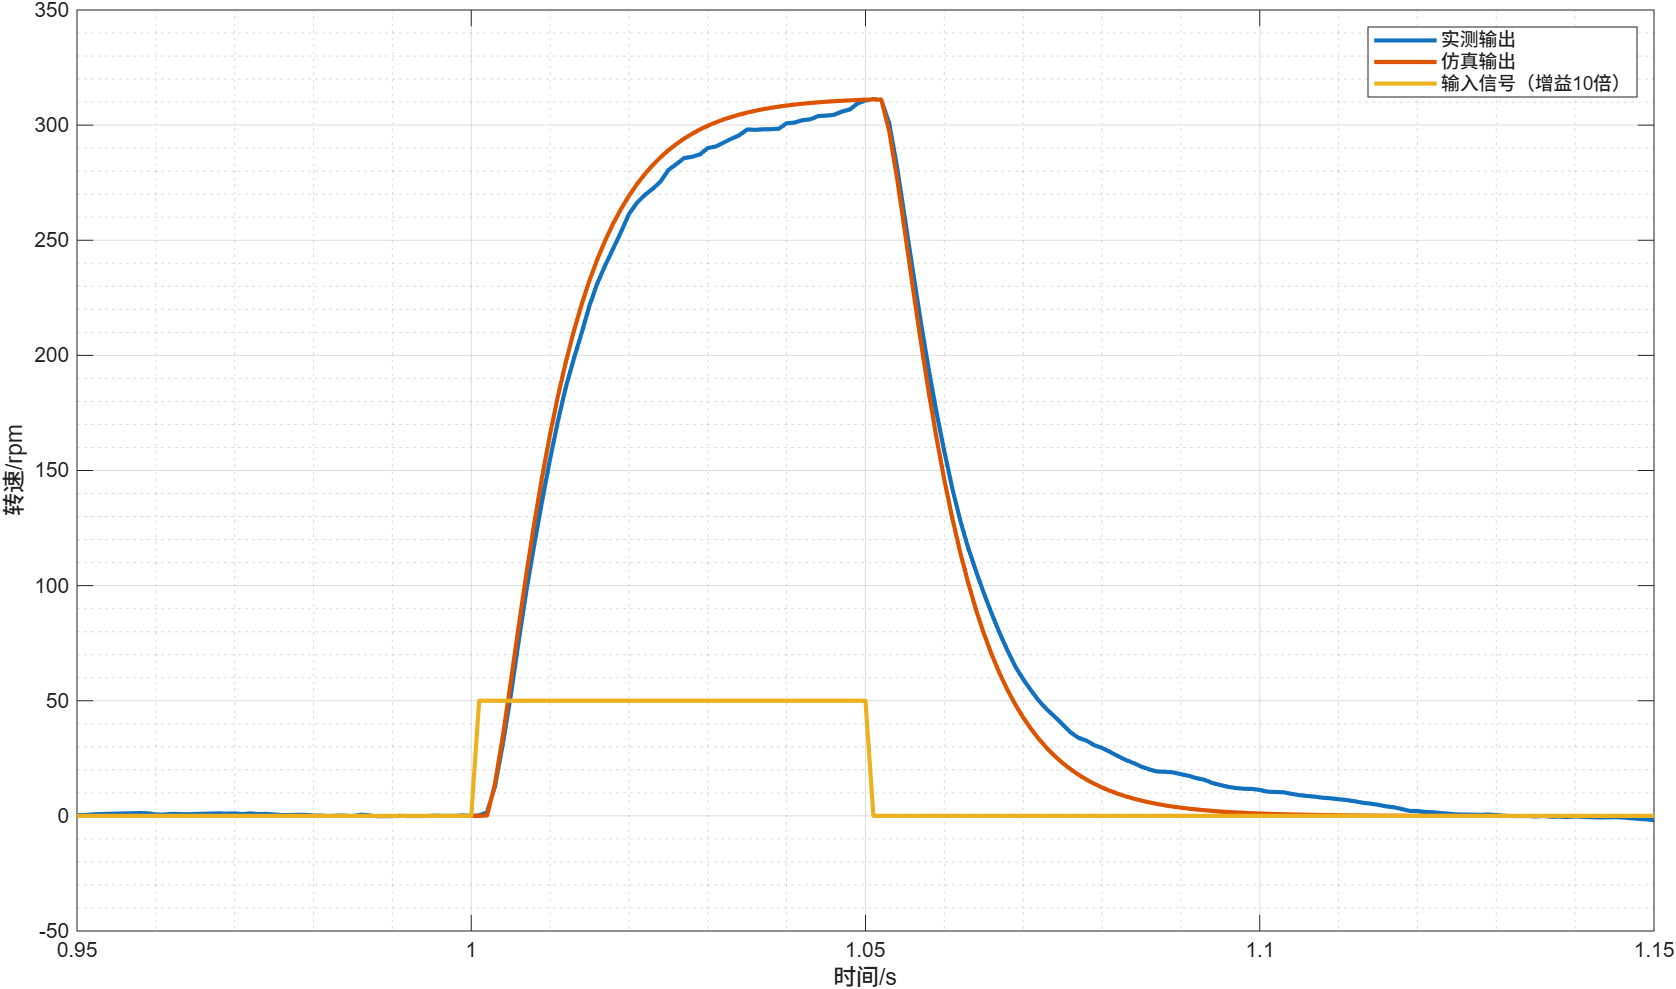
\includegraphics[width=0.6\textwidth]
    {图片/速度环正向方波转速对比.png}
    \caption{速度环正向方波转速对比}
    \label{fig:速度环正向方波转速对比}
\end{figure}

两个时域波形的相关系数99.85915\%，拟合优度93.11630\%。

负向方波作用下电动势和电磁转矩波形如下图所示。
\begin{figure}[H]
    \begin{minipage}{0.5\textwidth}
        \centering
        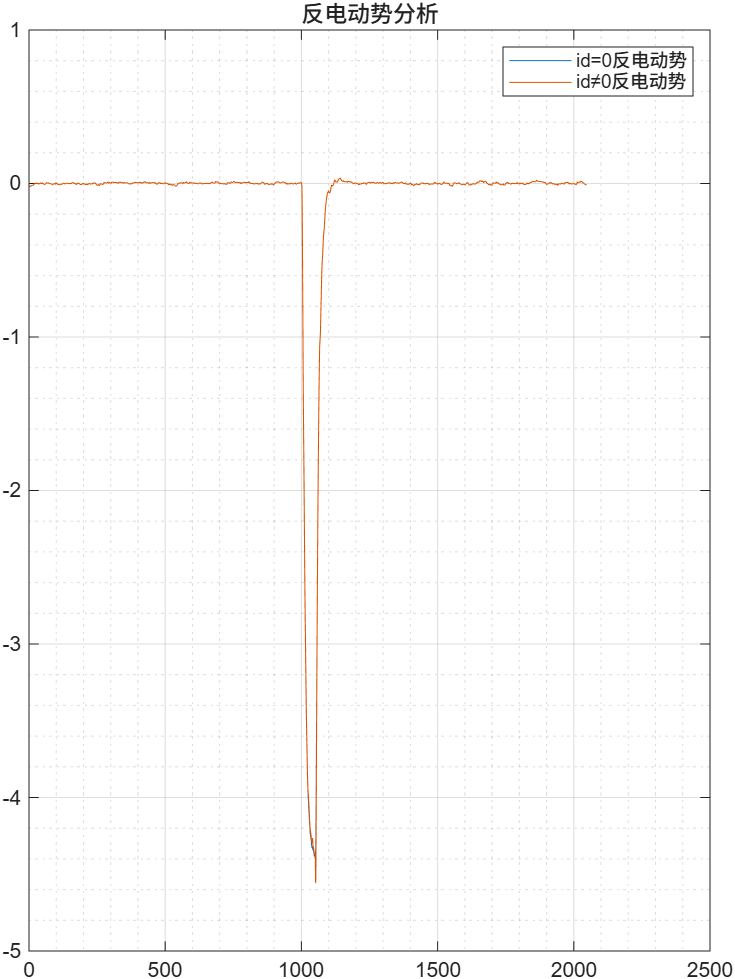
\includegraphics[width=\textwidth]
        {图片/速度环负向方波反电动势对比.png}
        \caption{速度环负向方波反电动势对比}
    \end{minipage}
    \begin{minipage}{0.5\textwidth}
        \centering
        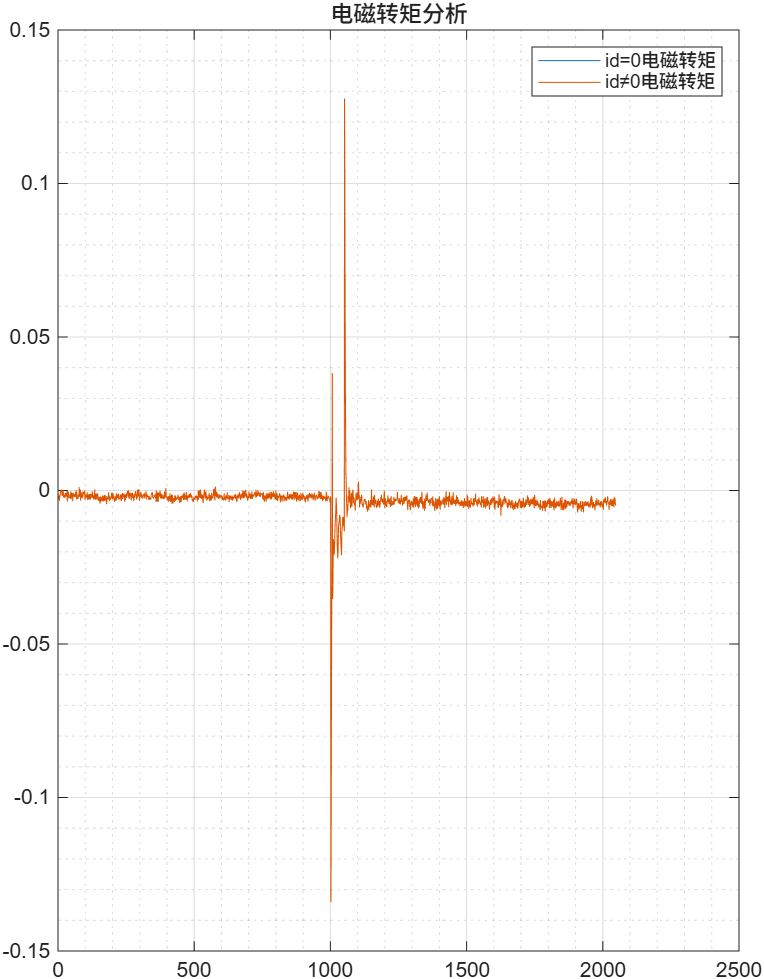
\includegraphics[width=\textwidth]
        {图片/速度环负向方波电磁转矩对比.png}
        \caption{速度环负向方波电磁转矩对比}
    \end{minipage}
    \label{fig:速度环负向方波理想id与实际id对比}
\end{figure}

分析可得反电动势相关系数99.99990\%，拟合优度99.84985\%；电磁转矩相关系数99.99999\%，拟合优度99.95191\%为极高水平，
同样遵守\(i_{\mathrm{d}}=0\)的理想化假设。此时仿真和实测的转速波形如下图所示。
\begin{figure}[H]
    \centering
    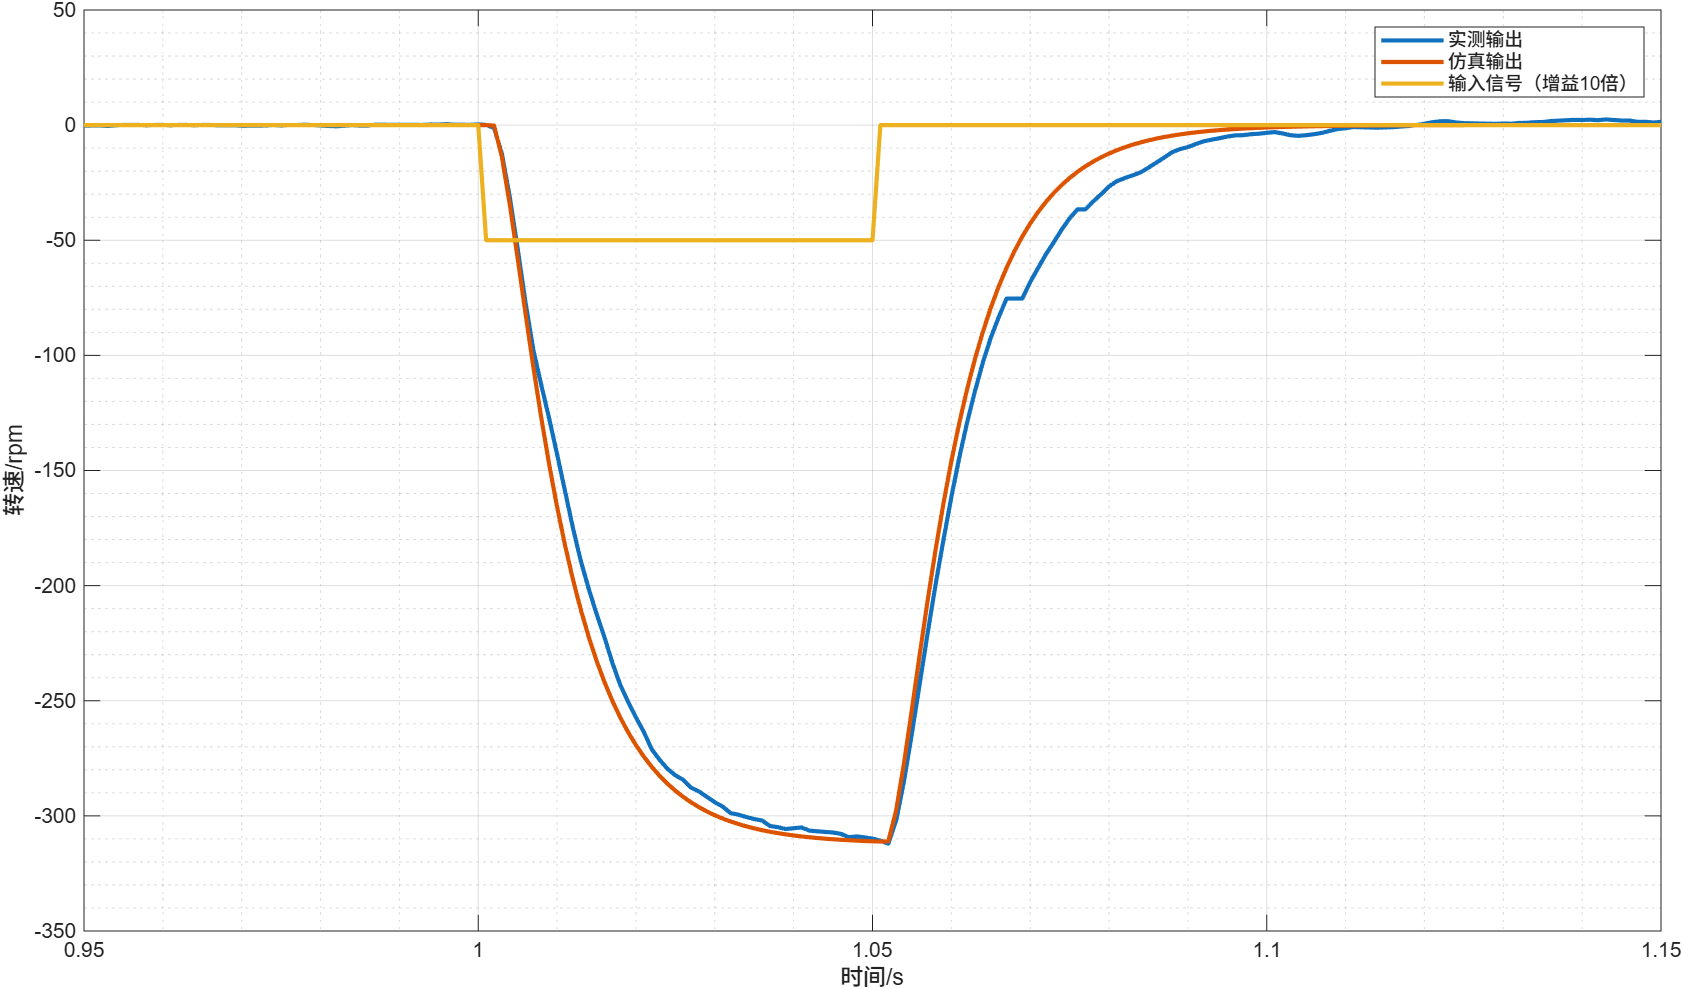
\includegraphics[width=0.6\textwidth]
    {图片/速度环负向方波转速对比.png}
    \caption{速度环负向方波转速对比}
    \label{fig:速度环负向方波转速对比}
\end{figure}

两个时域波形的相关系数99.92870\%，拟合优度95.71185\%。

据图\ref{fig:速度环正向方波转速对比}和图\ref{fig:速度环负向方波转速对比}可知，在暂态响应段仿真和实测波形高度一致。
而接近稳态时角加速度趋零，惯性力矩\(J\cfrac{\dd n}{\dd t}\)随之消失，齿槽转矩作为周期性扰动在速度波形上显现出来，
但振荡的均值与仿真波形的均值一致。说明建立的系统模型能够较为准确地解释电机的响应，但对非线性的齿槽转矩确实无法实现建模。

\subsection{速度环频域矫正控制器设计与闭环验证}
\subsubsection{速度环被控对象建模}
速度环频域矫正控制器仍采用与电流环相同的带积分环节超前校正结构，但被控对象不同于电流环的纯RL电路，
需要考虑反电动势反馈路径的物理存在。

在\ref{sec:电流环频域矫正控制器设计}中Q轴电流环控制器\(C_{\mathrm{q}}(s)\)按被控对象为纯RL电路模型\(\cfrac{1}{R_{\mathrm{s}}+L_{\mathrm{q}} s}\)设计，
并通过方波短脉冲测试（0.33ms内转速不发生明显变化）验证了该设计的有效性。但在速度环闭环控制中，转速\(n\)在秒级时间内大幅变化，
反电动势\(\omega_{\mathrm{e}}\psi_{\mathrm{m}}\)随转速动态变化，不再能视为常数扰动。此时从电流给定\(i_{\mathrm{q}}^*\)到转速\(n\)的物理被控对象包含反电动势反馈路径，
其传递函数为：

\begin{equation*}
    G_{\text{speed}}(s)=\cfrac{n(s)}{i_{\mathrm{q}}^*(s)}=
    \cfrac{C_{\mathrm{q}}(s)\times\cfrac{1}{R_{\mathrm{s}}+L_{\mathrm{q}} s}\times\cfrac{3}{2}p\psi_{\mathrm{m}}\times G_{\mathrm{m}}(s)}
    {1+\cfrac{\pi}{30}p\psi_{\mathrm{m}}\times\cfrac{1}{R_{\mathrm{s}}+L_{\mathrm{q}} s}\times\cfrac{3}{2}p\psi_{\mathrm{m}}\times G_{\mathrm{m}}(s)
    +C_{\mathrm{q}}(s)\times\cfrac{1}{R_{\mathrm{s}}+L_{\mathrm{q}} s}}
\end{equation*}

代入平均模型\eqref{eq:Gm参考模型}，进行ZOH按照采样频率1kHz离散化后经过低通滤波器\(F(z)=\cfrac{0.1}{1-0.9z^{-1}}\)，
可得等价离散化被控对象模型：
\begin{equation*}
    G_{\mathrm{s}}(z)=
    \cfrac{
        \begin{array}[t]{@{}l@{}}
            3.389 z^{-1} + 0.2123 z^{-2} - 14.06 z^{-3} + 15.6 z^{-4} - 6.191 z^{-5} + 1.179 z^{-6} \\
            - 0.1164 z^{-7} + 0.005744 z^{-8} - 0.0001118 z^{-9} + 1.374\times 10^{-9}z^{-10} - 1.141\times 10^{-19}z^{-11}
        \end{array}}
        {
        \begin{array}[t]{@{}l@{}}
            1 - 4.386 z^{-1} + 7.816 z^{-2} - 7.259 z^{-3} + 3.775 z^{-4} - 1.12 z^{-5} + 0.193 z^{-6} \\
            - 0.01891 z^{-7} + 0.0009637 z^{-8} - 1.967\times 10^{-5} z^{-9} + 1.963\times 10^{-10} z^{-10} - 7.451\times 10^{-16} z^{-11} \\
            + 6.191\times 10^{-26}z^{-12}
        \end{array}}
\end{equation*}

此时的双闭环控制系统框图如下图所示：

\begin{figure}[H]
    \centering
    \begin{tikzpicture}[auto, node distance=1.75cm, >=latex']
        % 样式定义
        \tikzstyle{block} = [draw, rectangle, minimum height=3em, minimum width=1.8em, align=center, inner sep=2pt]
        \tikzstyle{sum} = [draw, circle, node distance=1.5cm, minimum size=0.35em, inner sep=0pt]
        \tikzstyle{input} = [coordinate]
        \tikzstyle{output} = [coordinate]
        \tikzstyle{feedback} = [coordinate]

        % 放置节点
        \node [input, name=input] {};
        \node [sum, right of=input] (sum1) {};
        \node [block, right of=sum1] (Cs) {\(C_{\mathrm{s}}(s)\)};
        \node [sum, right of=Cs] (sum2) {};
        \node [block, right of=sum2] (Cq) {\(C_{\mathrm{q}}(s)\)};
        \node [sum, right of=Cq] (sum) {};
        \node [block, right of=sum] (RL) {\(\cfrac{1}{R_{\mathrm{s}}+L_{\mathrm{q}} s}\)};
        \node [block, right of=RL] (K) {\(\cfrac{3}{2}p\psi_{\mathrm{m}}\)};
        \node [block, right of=K] (Mech) {\(G_{\mathrm{m}}(s)\)};
        \node [block, right of=Mech] (ZOH) {ZOH};
        \node [block, right of=ZOH] (Filter) {\(\cfrac{0.1}{1-0.9z^{-1}}\)};
        \node [output, right of=Filter] (output) {};
        \node [block, below of=Mech, node distance=1.5cm] (Kf) {\(\cfrac{\pi}{30}p\psi_{\mathrm{m}}\)};
        \node [feedback, below of=sum, node distance=3.5cm] (F) {};
        \node [feedback, below of=Cq,node distance=2.5cm] (Fb) {};

        \draw [->] (input) -- node {\(n^*\)} (sum1);
        \draw [->] (sum1) -- node {\(\Delta n\)} (Cs);
        \draw [->] (Cs) -- node {\(i_{\mathrm{q}}^*\)} (sum2);
        \draw [->] (sum2) -- node {\(\Delta i_{\mathrm{q}}\)} (Cq);
        \draw [->] (Cq) -- node {\(U_{\mathrm{q}}\)} (sum);
        \draw [->] (sum) -- node {} (RL);
        \draw [->] (RL) -- node [name=iq] {\(i_{\mathrm{q}}\)} (K);
        \draw [->] (K) -- node {\(T_{\mathrm{e}}\)} (Mech);
        \draw [->] (Mech) -- node [name=y] {\(n\)} (ZOH);
        \draw [->] (ZOH) -- node {} (Filter);
        \draw [->] (Filter) -- node [name=y_fi] {\(\hat{n}\)} (output);
        % 反电动势反馈
        \draw [->] (y) |- (Kf);
        \draw [->] (Kf) -| node[pos=0.9] {\(-\)} node [pos=0.6] {\(E\)} (sum);
        % i_{\mathrm{q}}反馈：在交叉点处加桥接小弧（跳线），与反电动势线路交叉但不连接
        \coordinate (cross) at (iq |- Kf);
        \coordinate (jT) at ([yshift=0.12cm] cross);
        \coordinate (jB) at ([yshift=-0.12cm] cross);
        \draw [-] (iq) -- (jT);
        \draw [-] (jT) -- ++(0.12, -0.1) -- ++(0, -0.04) -- ++(-0.12, -0.1);
        \draw [-] (jB) |- (Fb);
        \draw [->] (Fb) -| node[pos=0.9] {\(-\)} node [pos=0.6] {} (sum2);
        \draw [-] (y_fi) |- (F);
        \draw [->] (F) -| node[pos=0.9] {\(-\)} node [pos=0.6] {} (sum1);
    \end{tikzpicture}
    \caption{Q轴双闭环控制系统框图}
    \label{fig:Q轴双闭环控制系统框图}
\end{figure}

\subsubsection{控制器设计与闭环验证}
为了实现无静差跟踪，在被控对象前串入积分环节。构成等价被控对象，开环伯德图如下图所示。
\begin{figure}[H]
    \centering
    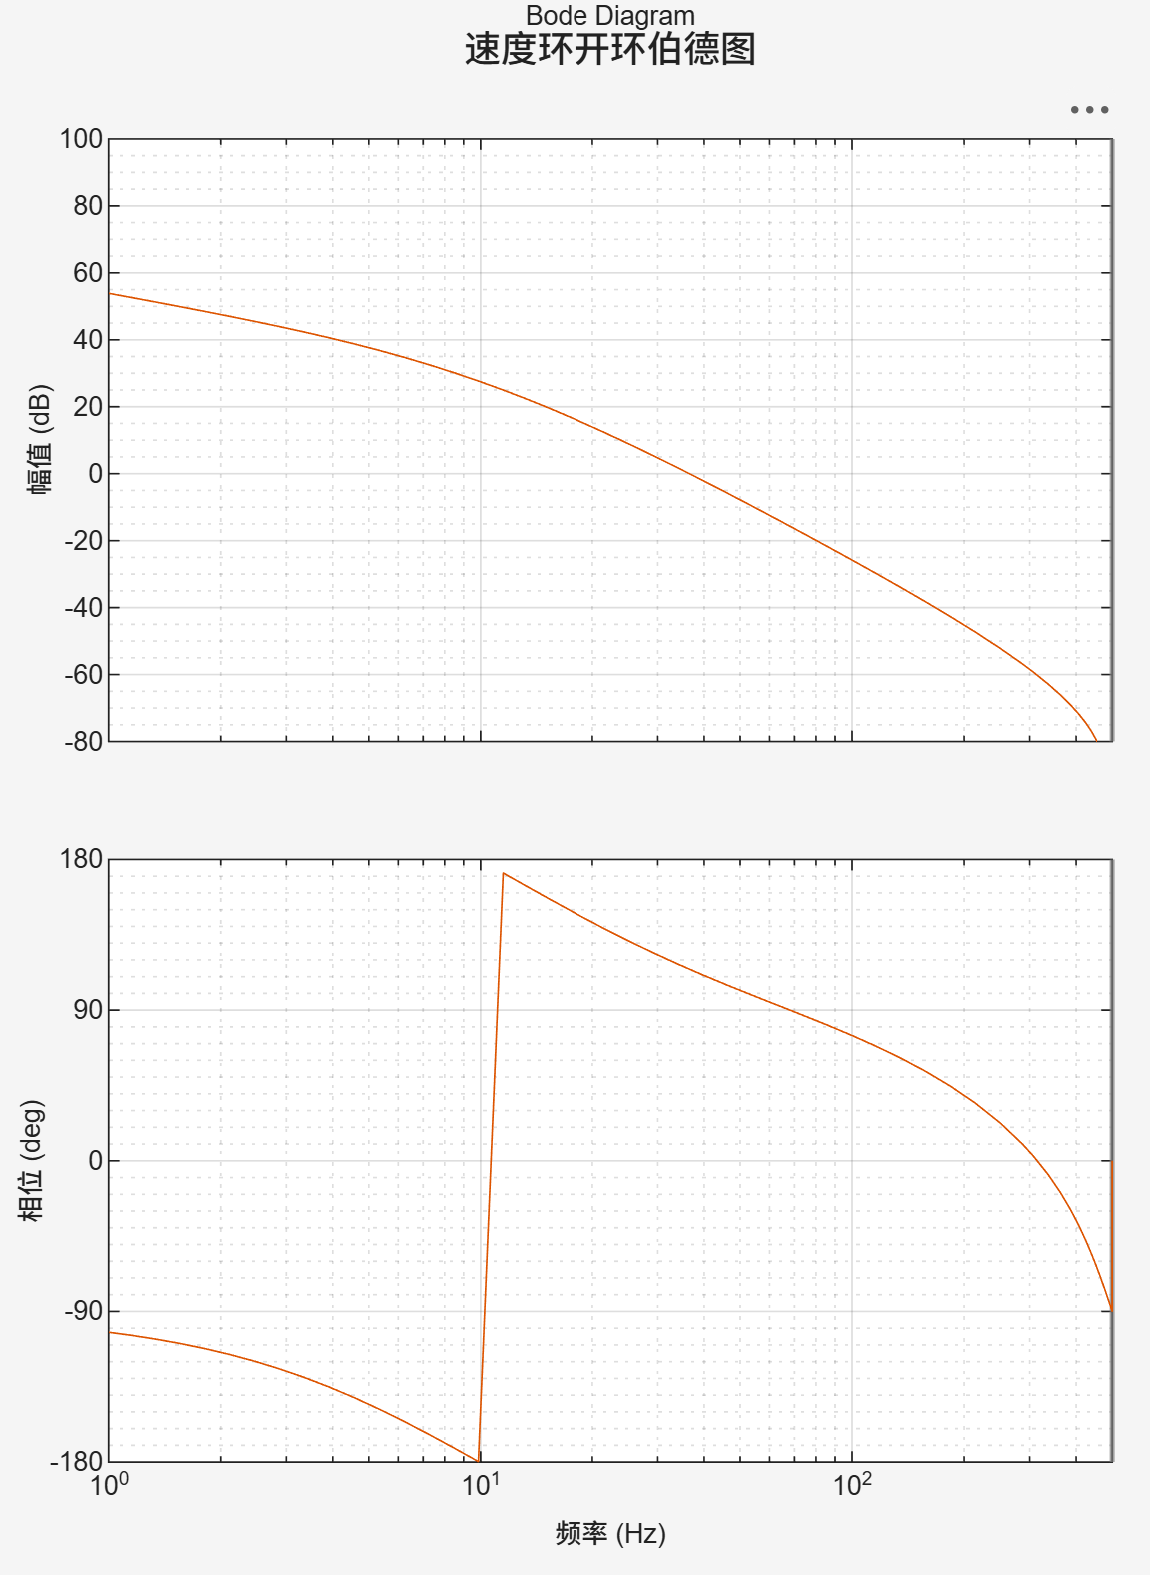
\includegraphics[width=0.5\textwidth]
    {图片/带积分环节的速度环等价被控对象开环频率特性.png}
    \caption{带积分环节的速度环等价被控对象开环频率特性}
\end{figure}

与电流环控制器一样，采用一阶超前校正控制\(C_{\mathrm{s}}(s)=K\cfrac{Ts+1}{\alpha Ts+1}\)，开环截止频率设定为13Hz，
以不低于40°的相位裕度为目标，在13Hz处提供最多65°的相位补偿，可以计算得到：
\begin{equation*}
    \begin{cases}
        \alpha = \cfrac{1-\sin(65°)}{1+\sin(65°)}=0.0491\\
        T = \cfrac{1}{2\pi\times 12\sqrt{\alpha}} = 0.0552
    \end{cases}
\end{equation*}

最后根据等价被控对象在12Hz处的增益，调整放大系数K，最终可得带积分的速度环超前控制器：
\begin{equation*}
    C_{\mathrm{s}}(s)=\cfrac{0.0008946s+0.0162}{0.002714s^2+s}
\end{equation*}

使用双线性变换离散化后得到：
\begin{equation*}
    C_{\mathrm{s}}(z)=\cfrac{0.0001404+2.52\times 10^{-6}z^{-1}-0.0001379z^{-2}}{1-1.6889z^{-1}+0.6889z^{-2}}
\end{equation*}

经过超前控制后的开环频率特性和闭环频率特性如下图所示。
\begin{figure}[H]
    \centering
    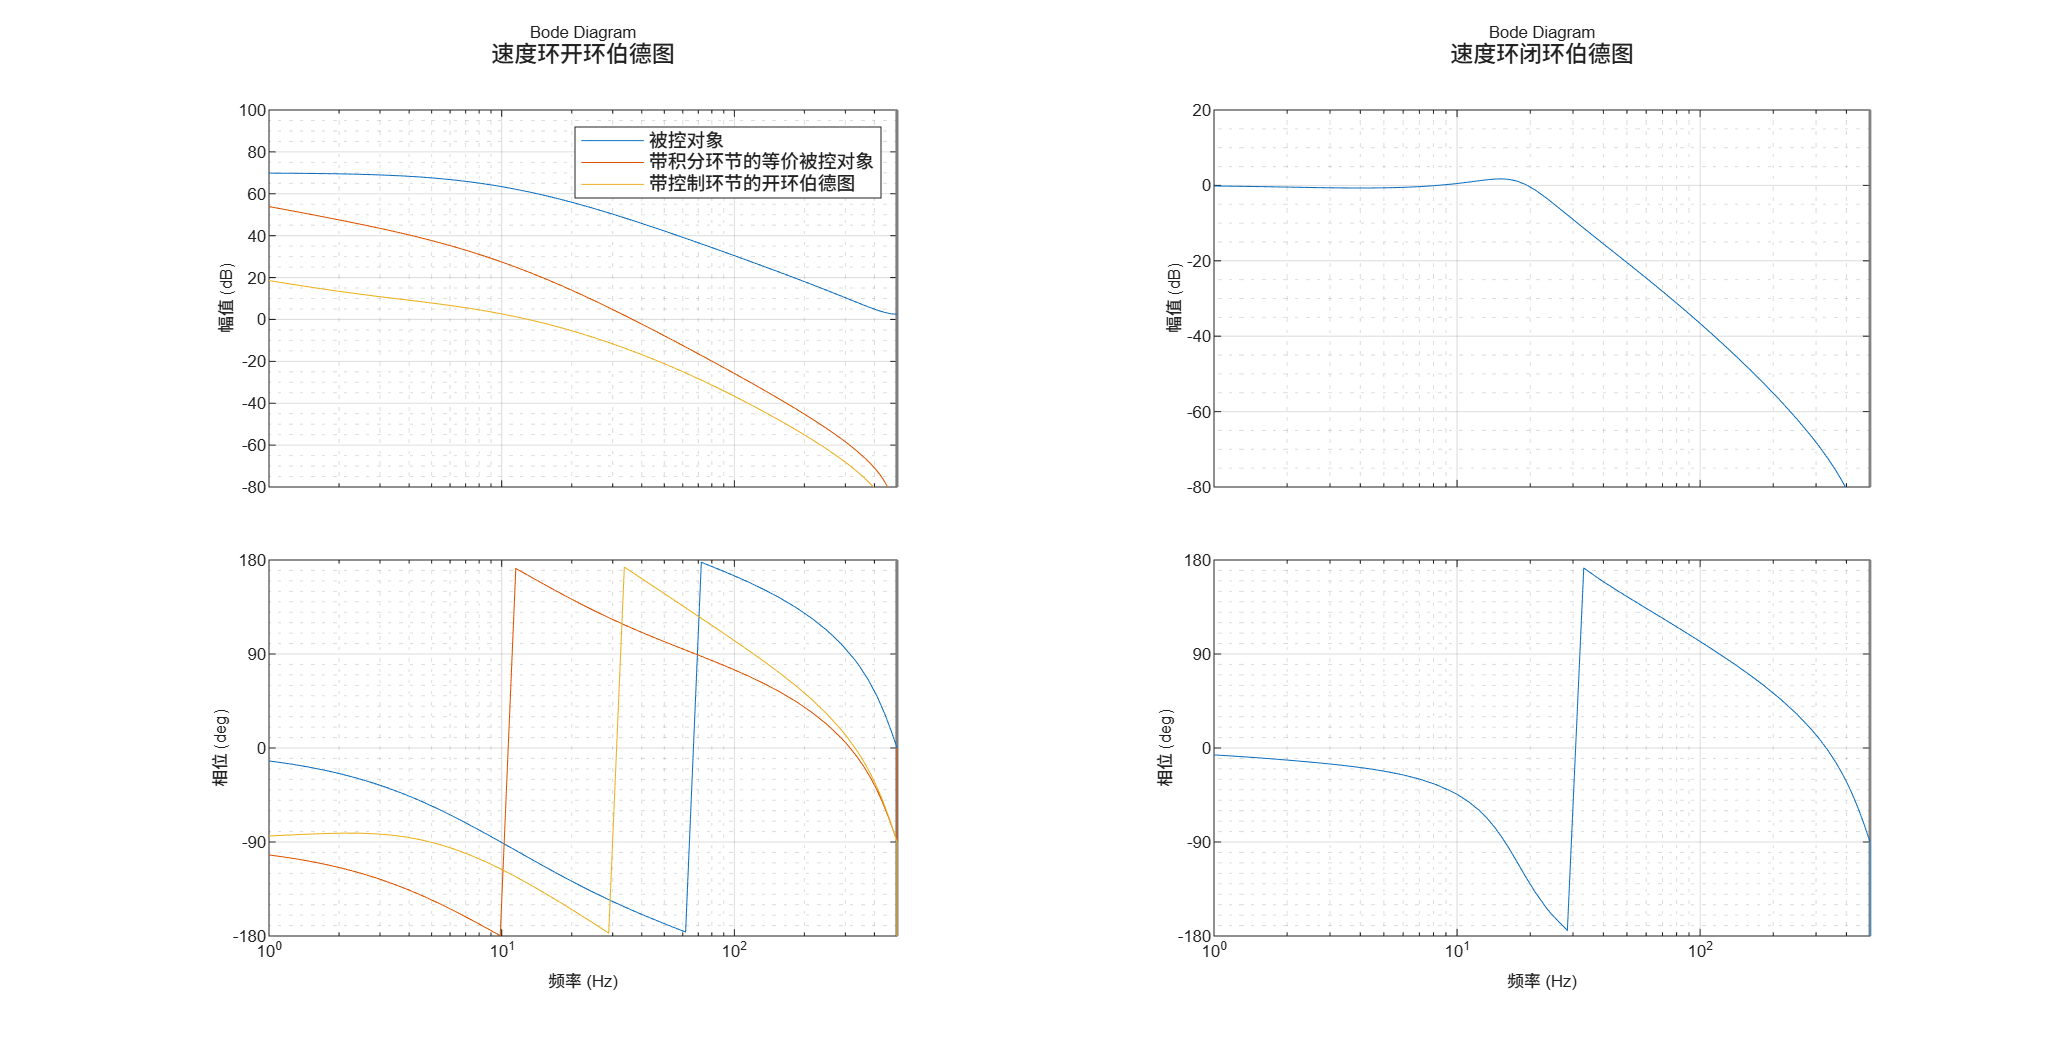
\includegraphics[width=\textwidth]
    {图片/速度环开-闭环频率特性.png}
    \caption{速度环开-闭环频率特性}
\end{figure}

矫正后，速度环的开环截止频率13Hz，相位裕度50.21128°满足设计要求。相位穿越频率30.14228Hz，
幅值裕度11.75946dB，闭环带宽22.95915Hz。闭环前后的单位阶跃响应如下图所示。
\begin{figure}[H]
    \centering
    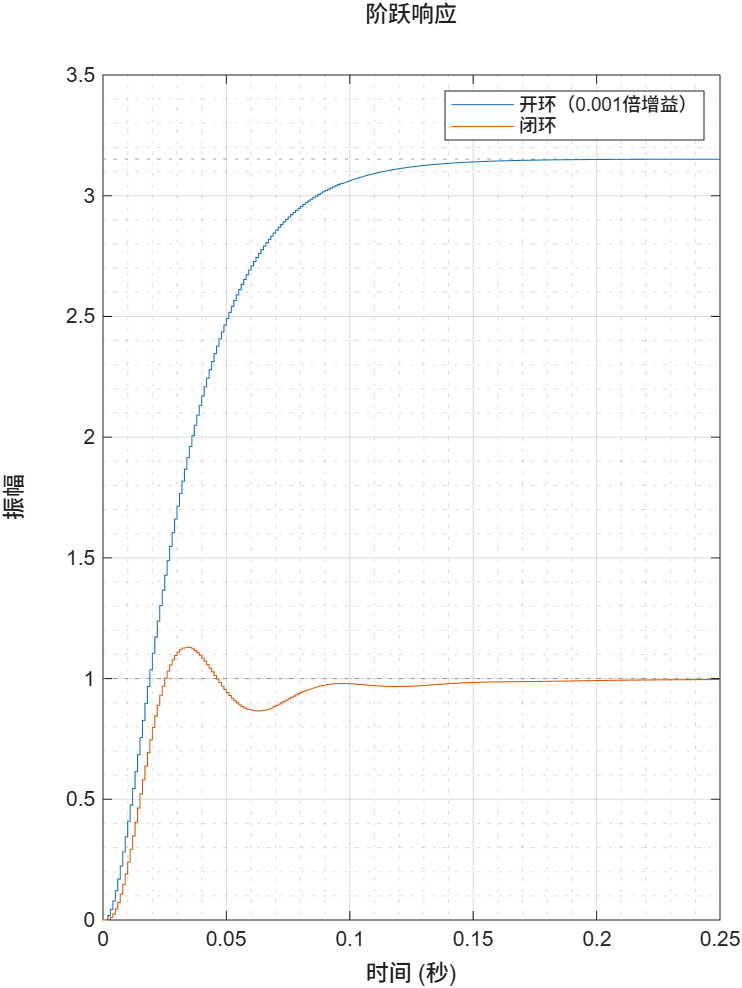
\includegraphics[width=0.5\textwidth]
    {图片/速度环开-闭环单位阶跃响应对比.png}
    \caption{速度环开-闭环单位阶跃响应对比}
\end{figure}

可以发现，通过带积分环节的超前校正控制器，使得能够无差跟踪给定信号，超调量13\%，调节时间为0.142s，用一定的超调
换来了极快的响应速度。接下来考虑以±150rpm的方波速度给定信号（持续500个采样周期）进行测试，以评估实际系统响应和
建模准确性，结果如下图所示。
\begin{figure}[H]
    \begin{minipage}{0.5\textwidth}
        \centering
        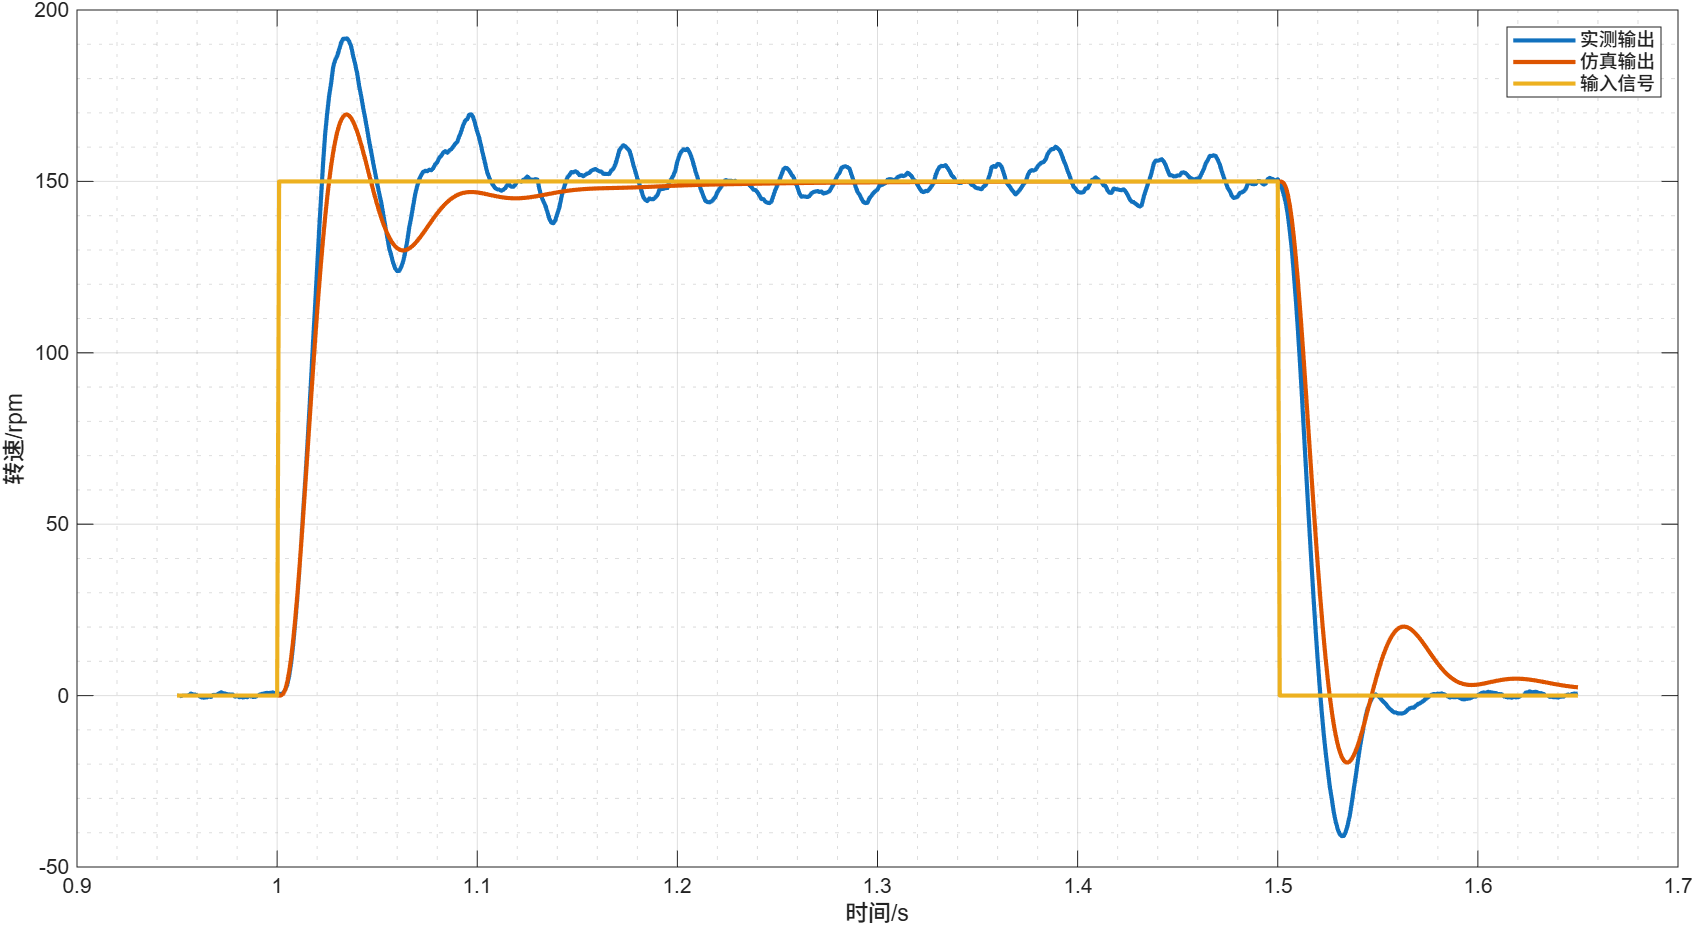
\includegraphics[width=\textwidth]
        {图片/速度环正向方波闭环验证.png}
        \caption{速度环正向方波闭环验证}
    \end{minipage}
    \begin{minipage}{0.5\textwidth}
        \centering
        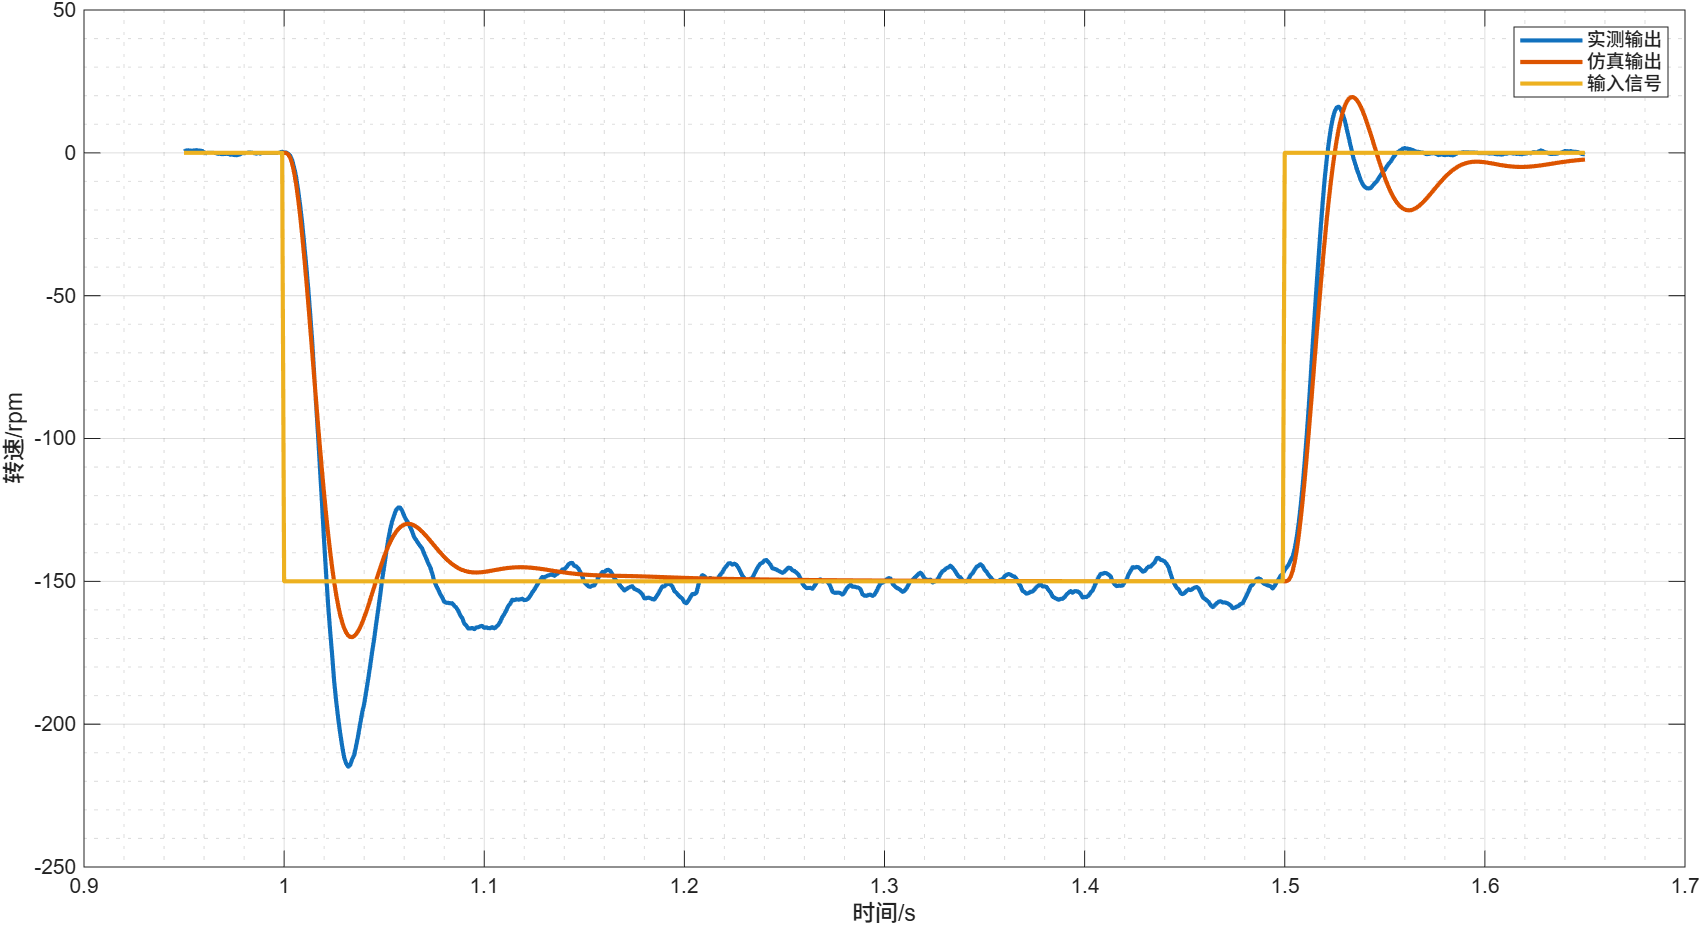
\includegraphics[width=\textwidth]
        {图片/速度环负向方波闭环验证.png}
        \caption{速度环负向方波闭环验证}   
    \end{minipage}
\end{figure}

与开环验证结果类似，仿真和实测波形在暂态段基本一致。进入稳态后惯性力矩趋于零，
齿槽转矩作为周期性扰动凸显出来，此时即使用闭环控制器也无法完全消除其带来的转速振荡，因此稳态段偏差较大。
正向方波相关系数99.34643\%，拟合优度86.99273\%；
负向方波相关系数99.05066\%，拟合优度85.20157\%，拟合水平低于电流闭环验证。
原因有三：其一，速度回路的非线性干扰强度和来源均高于电路部分，线性传递函数的拟合精度天然更低；
其二，速度环辨识在Q轴电流闭环下进行，闭环效应（积分饱和、输出限幅）使系统特性较开环时更为复杂，降低了验证结果的准确性；
其三，电路部分有明确的解析结构（一阶RL电路），可据此修正辨识偏差，而速度环被控对象即使采用
经典的\(\cfrac{1}{Js+B}\)模型，也在该电机上存在显著的不适配。
需要说明的是，闭环验证拟合优度低于开环验证并非表明辨识结果更不可信：如\ref{sec:反推结果的敏感性分析}所述，
开环验证的拟合优度主要受极低频段（直流稳态）误差拖累，而闭环验证中该误差被速度环积分环节压制，
剩余偏差主要源于核心频段模型误差与速度测量噪声的反馈放大，以及上述三点原因。因此闭环验证拟合优度
有所降低属预期现象，模型可信度仍由开环验证确立。整体上拟合优度均大于85\%，仍属可接受范围。

最后，在上述测试过程中对\(i_{\mathrm{d}}=0\)的理想化假设验证如下图所示。
正向方波闭环测试过程中，反电动势相关系数99.99993\%，拟合优度99.88057\%；电磁转矩相关系数100.00000\%，拟合优度99.97844\%；
负向方波闭环测试过程中，反电动势相关系数99.99992\%，拟合优度99.87166\%；电磁转矩相关系数100.00000\%，拟合优度99.98025\%。
\begin{figure}[H]
    \begin{minipage}{0.5\textwidth}
        \centering
        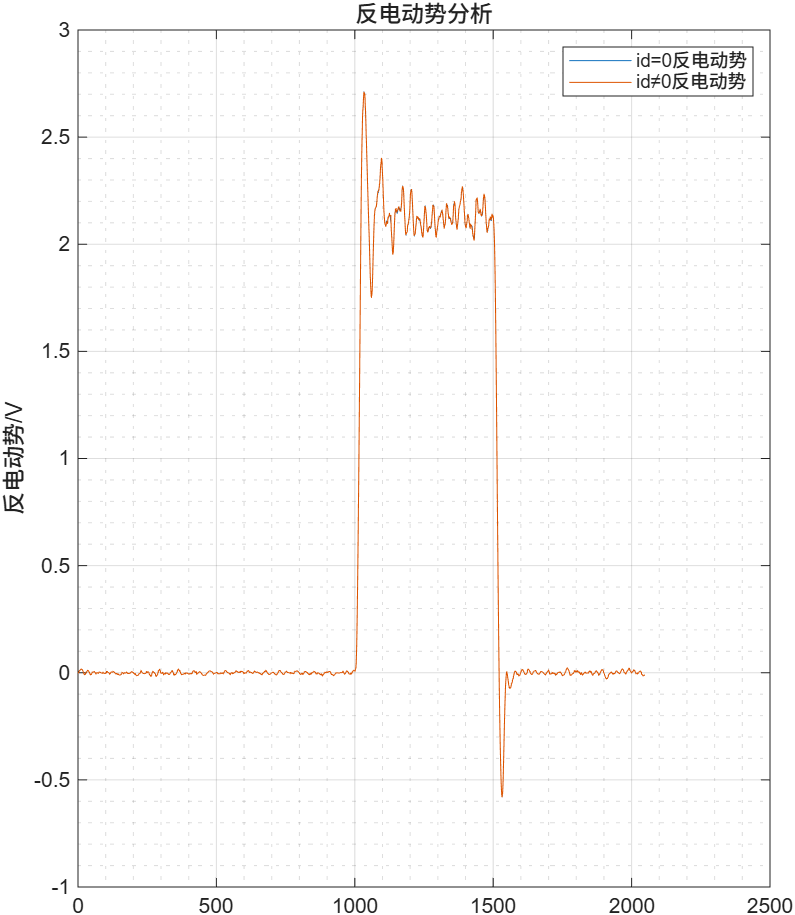
\includegraphics[width=\textwidth]
        {图片/速度环正向闭环方波反电动势对比.png}
        \caption{速度环正向闭环方波反电动势对比}
    \end{minipage}
    \begin{minipage}{0.5\textwidth}
        \centering
        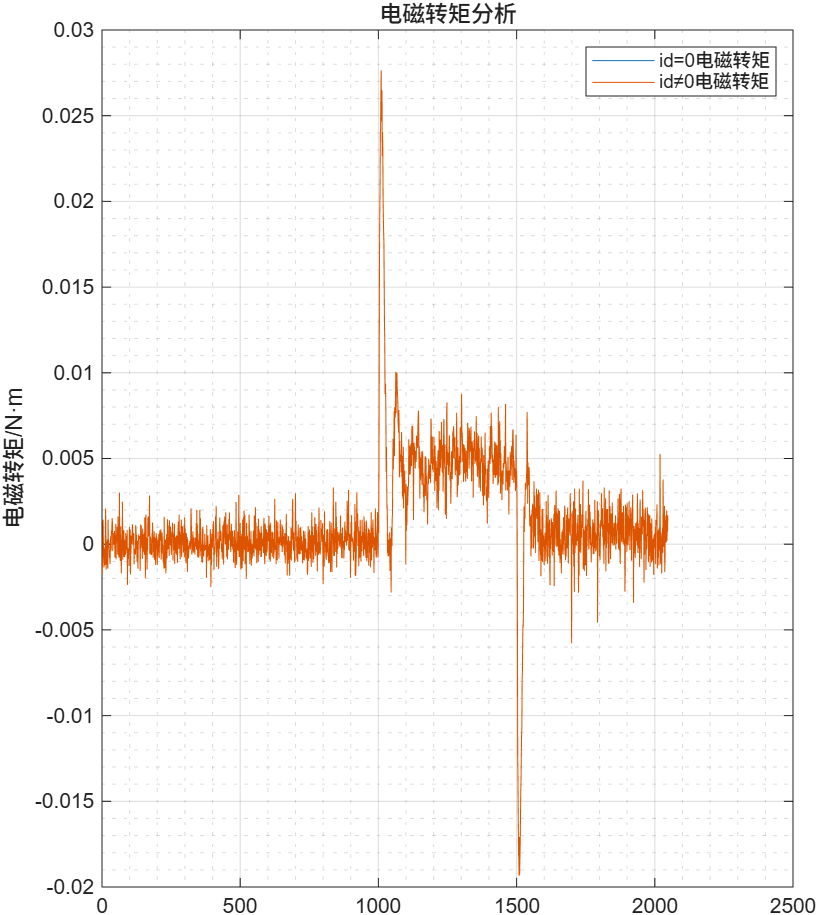
\includegraphics[width=\textwidth]
        {图片/速度环正向闭环方波电磁转矩对比.png}
        \caption{速度环正向闭环方波电磁转矩对比}
    \end{minipage}
\end{figure}
\begin{figure}[H]
    \begin{minipage}{0.5\textwidth}
        \centering
        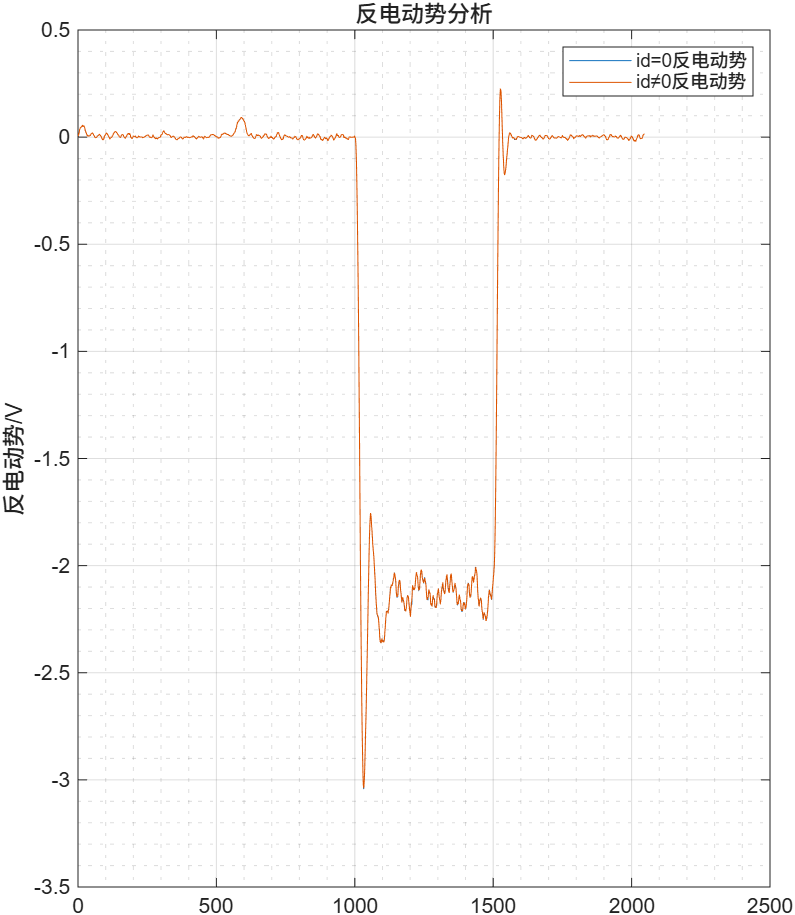
\includegraphics[width=\textwidth]
        {图片/速度环负向闭环方波反电动势对比.png}
        \caption{速度环负向闭环方波反电动势对比}
    \end{minipage}
    \begin{minipage}{0.5\textwidth}
        \centering
        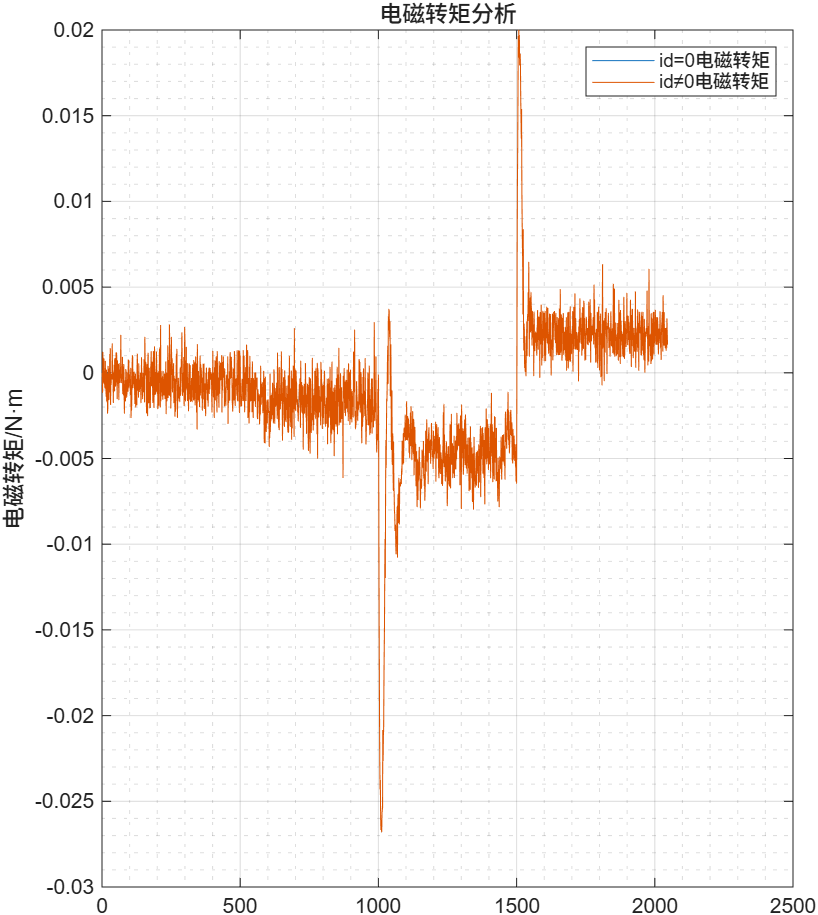
\includegraphics[width=\textwidth]
        {图片/速度环负向闭环方波电磁转矩对比.png}
        \caption{速度环负向闭环方波电磁转矩对比}
    \end{minipage}
\end{figure}

\subsubsection{反电动势前馈补偿分析}
上述测试证实了在\(i_{\mathrm{d}}=0\)控制下反电动势与电磁转矩的理想化假设均成立，且模型精度极高。
那么进行反电动势前馈补偿，以进一步改善速度环响应应当是可行的。
为此，在\(C_{\mathrm{Q}}(s)\)输出端叠加前馈项\(\hat{E}=\cfrac{\pi}{30}np\hat{\psi}_{\mathrm{m}}\)，加入前馈后的系统框图如下图所示。
\begin{figure}[H]
    \centering
    \begin{tikzpicture}[auto, node distance=1.75cm, >=latex']
        % 样式定义
        \tikzstyle{block} = [draw, rectangle, minimum height=3em, minimum width=1.8em, align=center, inner sep=2pt]
        \tikzstyle{sum} = [draw, circle, node distance=1.5cm, minimum size=0.35em, inner sep=0pt]
        \tikzstyle{input} = [coordinate]
        \tikzstyle{output} = [coordinate]
        \tikzstyle{feedback} = [coordinate]

        % 放置节点
        \node [input, name=input] {};
        \node [sum, right of=input] (sum1) {};
        \node [block, right of=sum1] (Cs) {\(C_{\mathrm{s}}(s)\)};
        \node [sum, right of=Cs] (sum2) {};
        \node [block, right of=sum2] (Cq) {\(C_{\mathrm{q}}(s)\)};
        \node [sum, right of=Cq] (sum) {};
        \node [block, right of=sum] (RL) {\(\cfrac{1}{R_{\mathrm{s}}+L_{\mathrm{q}} s}\)};
        \node [block, right of=RL] (K) {\(\cfrac{3}{2}p\psi_{\mathrm{m}}\)};
        \node [block, right of=K] (Mech) {\(G_{\mathrm{m}}(s)\)};
        \node [block, right of=Mech] (ZOH) {ZOH};
        \node [block, right of=ZOH] (Filter) {\(\cfrac{0.1}{1-0.9z^{-1}}\)};
        \node [output, right of=Filter] (output) {};
        \node [block, below of=Mech, node distance=1.5cm] (Kf) {\(\cfrac{\pi}{30}p\psi_{\mathrm{m}}\)};
        \node [feedback, below of=sum, node distance=3.5cm] (F) {};
        \node [feedback, below of=Cq,node distance=2.5cm] (Fb) {};
        \node [block, above of=ZOH, node distance=1.5cm] (FF) {\(\cfrac{\pi}{30}p\hat{\psi}_{\mathrm{m}}\)};

        \draw [->] (input) -- node {\(n^*\)} (sum1);
        \draw [->] (sum1) -- node {\(\Delta n\)} (Cs);
        \draw [->] (Cs) -- node {\(i_{\mathrm{q}}^*\)} (sum2);
        \draw [->] (sum2) -- node {\(\Delta i_{\mathrm{q}}\)} (Cq);
        \draw [->] (Cq) -- node {\(U_{\mathrm{q}}\)} (sum);
        \draw [->] (sum) -- node {} (RL);
        \draw [->] (RL) -- node [name=iq] {\(i_{\mathrm{q}}\)} (K);
        \draw [->] (K) -- node {\(T_{\mathrm{e}}\)} (Mech);
        \draw [->] (Mech) -- node [name=y] {\(n\)} (ZOH);
        \draw [->] (ZOH) -- node {} (Filter);
        \draw [->] (Filter) -- node [name=y_fi] {\(\hat{n}\)} (output);
        % 反电动势反馈
        \draw [->] (y) |- (Kf);
        \draw [->] (Kf) -| node[pos=0.9] {\(-\)} node [pos=0.6] {\(E\)} (sum);
        % i_{\mathrm{q}}反馈：在交叉点处加桥接小弧（跳线），与反电动势线路交叉但不连接
        \coordinate (cross) at (iq |- Kf);
        \coordinate (jT) at ([yshift=0.12cm] cross);
        \coordinate (jB) at ([yshift=-0.12cm] cross);
        \draw [-] (iq) -- (jT);
        \draw [-] (jT) -- ++(0.12, -0.1) -- ++(0, -0.04) -- ++(-0.12, -0.1);
        \draw [-] (jB) |- (Fb);
        \draw [->] (Fb) -| node[pos=0.9] {\(-\)} node [pos=0.6] {} (sum2);
        \draw [-] (y_fi) |- (F);
        \draw [->] (F) -| node[pos=0.9] {\(-\)} node [pos=0.6] {} (sum1);
        \draw [->] (y_fi) |- (FF);
        \draw [->] (FF) -| node[pos=0.6] {\(\hat{E}\)} (sum);
    \end{tikzpicture}
    \caption{Q轴双闭环控制系统框图（带反电动势前馈）}
    \label{fig:Q轴双闭环控制系统框图（带反电动势前馈）}
\end{figure}

采用原先的控制器，分别测试在前馈补偿前后的方波响应，结果如下图所示。
\begin{figure}[H]
    \centering
    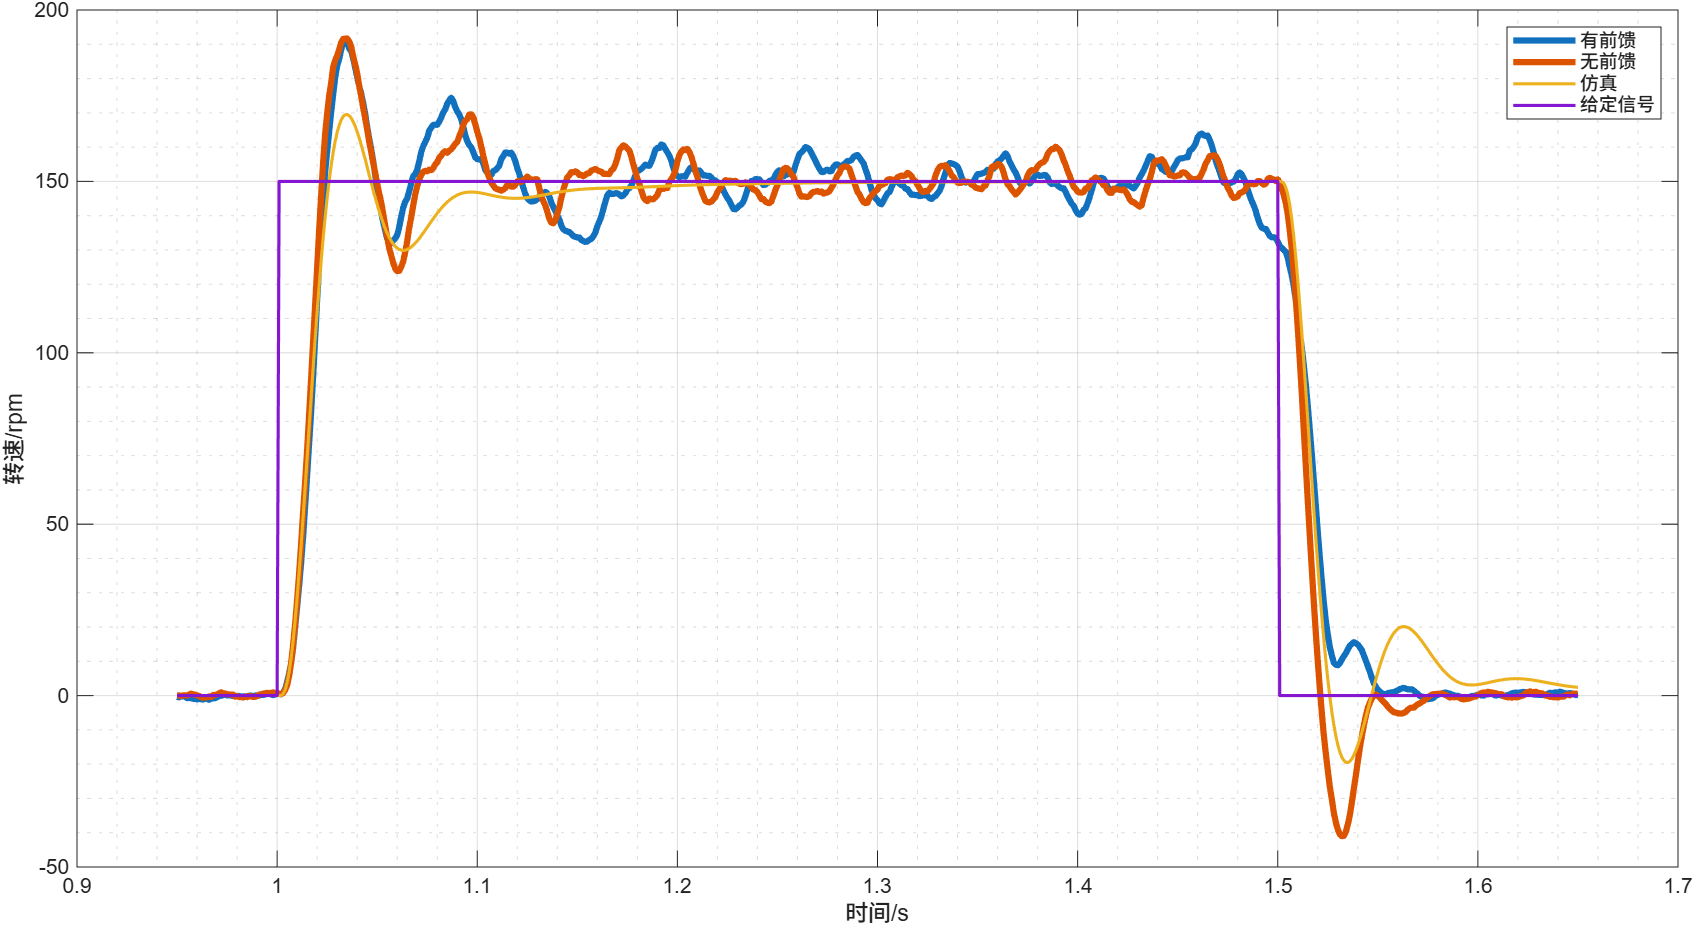
\includegraphics[width=\textwidth]
    {图片/前馈补偿对比.png}
    \caption{前馈补偿对比}
\end{figure}

可以发现，补偿前后响应有所改善，但没有达到质变的程度。
分析其原因在于反电动势在奇异摄动系统中的双重属性。对闭环带宽高达2kHz、控制采样频率15kHz的电流内环而言，反电动势
近似于缓慢变化的直流扰动（因为在设计时没有考虑），设计的控制器\(C_{\mathrm{Q}}(s)\)能够很好地压制其作用。而
对于闭环带宽仅21Hz、控制采样频率1kHz的速度外环而言，反电动势的变化正好落在其核心工作频段内。

上述双重属性带来了两个影响，其一是电流环控制器本身足以压制反电动势扰动，前馈补偿带来的收益有限；其二是对于速度环
被控对象设计而言反电动势的物理路径依然存在且不可忽略，求解速度环被控对象时仍然要在电流环和反电动势闭环耦合的情况下
进行。若直接忽视反电动势闭环简化被控对象求解，会过于乐观地轻视了被控对象的复杂特性，设计出的控制器基本不可用
\footnote{经测试，即使用很保守的参数设计控制器依然会导致系统发散}。

综上所述，本章采用的分步策略：电流环控制器设计、含反电动势的速度环建模、频域校正设计在电机控制器设计上是
更鲁棒的做法，而反电动势的前馈补偿在这其中并不是必要步骤。